\chapter{无线密钥生成系统的实验数据分析和验证}

本文已经介绍了无线密钥生成技术的理论基础,以及无线密钥生成系统的详细设计。目前大多数研究工作专注仿真较多,本文基于GNURadio软件无线电开发平台和USRP通用软件无线电外设,设计并实现了TDD/FDD模式下的高效无线密钥生成系统,并在实际环境下测量大量数据并验证。实际测量中的信道环境更加复杂,因此本文在室内房间、室内走廊和空旷室外三种场景下的终端固定、终端移动和人员走动三种不同信道环境下多次测量数据,并根据测量结果,分析合法通信双方和窃听者CSI的互易性、CSI信息泄漏率、CSI随机性、密钥随机性、密钥生成速率、Turbo纠错码以及BCH纠错码的BER等指标来验证无线密钥生成系统的可靠性和安全性。

\section{实验平台}

本文使用GNURadio软件无线电套件开发无线密钥生成系统。其中,系统中的信道测量依赖于USRP外设发射和接收数据,特征量化、信息调和、隐私放大在PC中处理完成,信息调和的信息交互在无线局域网中完成。无线密钥生成系统可以通过配置参数实现不同频点下、不同采样率下、TDD/FDD模式的无线密钥生成,并将接收导频信号、探测结果CSI、会话密钥等中间结果转存到磁盘。

本系统使用GNURadio版本为3.7.11,使用三台USRP N210作为外设,使用三台PC部署主机程序。USRP N210可以提供高带宽、高动态范围处理能力。USRP N210拥有Xilinx® Spartan® 3A-DSP 3400 FPGA,100 MS/s的双ADC,400 Ms/s的双DAC,和PC处理器之间通过千兆以太网连接用于通信,USRP N210和主机之间的通信速度可达50 MS/s。USRP N210可以工作在0\~6GHz,并且拥有允许多个USRP N210同步构建MIMO的扩展端口。USRP N210在发射和接收方向的处理能力达到100 MS/s。

如图\ref{system-three}所示,实验中分Alice、Bob、Eve三个角色,Alice和Bob是合法通信方,Eve是窃听者。三台PC共处一个无线局域网内,因为三者之间需要通过无线局域网进行信息调和,其中Alice事先已经得知Bob和Eve的无线局域网IP。如图\ref{system-usrp}所示,每一台PC均和一台USRP N210配置在同一个有线局域网内,PC和USRP之间依靠千兆以太网网口传输数据,本系统将PC的有线局域网IP配置为$192.168.10.1$,USRP的有线局域网IP配置为$192.168.10.2$。

本文使用主从模式来实现系统流程控制,无线密钥生成系统的密钥协商过程由主端控制,从端被动响应。Alice为主端,Bob和Eve均为从端。在一次信道探测过程中,主端Alice发起信道探测,从端Bob和Eve均会探测到导频信号,Bob会回发导频信号。之后三者各自分析计算CSI并生成密钥,Alice和Bob进一步调和生成会话密钥,并用于加密信息的传输。Eve由于接收到的导频信号经过不同的信道衰落,尽管经过相同的生成步骤,但是最终生成的密钥不同,因此无法破解消息。

\begin{figure}[htbp!]
    \centering \includegraphics[width=0.9\textwidth]{images/system-three}
    \caption{无线密钥生成系统平台}
    \label{system-three}
\end{figure}

\begin{figure}[htbp!]
    \centering \includegraphics[width=0.9\textwidth]{images/system-usrp}
    \caption{PC和USRP N210}
    \label{system-usrp}
\end{figure}

如图\ref{alice}所示为无线密钥生成系统的控制界面,系统左侧为系统参数栏,系统右侧为结果显示栏。表\ref{left-column-args}为左侧参数栏说明,右侧为CSI曲线、加密后图片、系统运行时间、已生成密钥数。

\begin{figure}[htbp!]
    \centering \includegraphics[width=0.9\textwidth]{images/alice}
    \caption{无线密钥生成系统的控制界面}
    \label{alice}
\end{figure}

\begin{table}[]
    \centering
    \begin{tabular}{|l|l|}
    \hline
    参数 & 说明 \\ \hline
    模式 & TDD/FDD \\ \hline
    角色 & alice/bob/eve \\ \hline
    CSI存储目录 & CSI存储位置 \\ \hline
    密钥存储目录 & 密钥存储位置 \\ \hline
    是否连续存储 & 密钥和CSI是否以追加方式存储 \\ \hline
    对等实体ip & 合法通信对方的无线局域网IP \\ \hline
    是否存在eve & 窃听方的无线局域网IP \\ \hline
    增益 & USRP增益 \\ \hline
    采样率 & USRP采样率 \\ \hline
    载波 & 载波频率 \\ \hline
    设备地址 & USRP的有线局域网IP \\ \hline
    \end{tabular}
    \caption{左侧参数说明
    \label{left-column-args}}
\end{table}
\
\section{场景架构}

% todo 记得把实际采数据的环境拍一下

本文在如图\ref{sketch_scene}所示的室内房间、室内走廊、空旷室外三种场景下使用无线密钥生成系统,并在不同场景下设计三种信道环境,

\begin{figure}
    \centering
    \subfigure[室内]{
      \includegraphics[width=0.9\textwidth]{images/indoor-experiment2.png}
    }
    \quad
    \subfigure[走廊]{
      \includegraphics[width=0.9\textwidth]{images/corridor-experiment2.png}
    }
    \quad
    \subfigure[室外]{
      \includegraphics[width=0.9\textwidth]{images/outdoor-experiment2.png}
    }
    \quad
    \caption{室内、走廊和室外的示意图}{}
    \label{sketch_scene}
\end{figure}

\begin{itemize}
    \item \textbf{方式1} 不干扰信道
    \item \textbf{方式2} 行人在周围环境随机移动
    \item \textbf{方式3} 收发机小范围内移动   
\end{itemize}

因此本文分别在TDD和FDD模式下,测量了9种实际情况下的信道环境,并分析无线密钥生成系统的可靠性和安全性。以下将分别探讨TDD和FDD模式下,无线密钥生成系统的性能。


  
\section{TDD模式}


本文在TDD模式下的9种情况中,连续长时间采取600组数据,用于实验结果分析。TDD模式下的试验参数如表\ref{tdd-exp-args}所示,即通信方在2535MHz的频点发射和接收导频信号,导频信号前后两端设有正弦波,Alice发射的导频信号的正弦波频率为4Hz,Bob发射的导频信号的正弦波频率为8Hz,两者使用相同的、长度为4095的M序列用于精同步和信道估计,USRP的采样率均设置为25 MHz。三个场景下、三种信道环境的600组CSI如图\ref{tdd_csi_ab}所示,图中只展示了Alice的结果。图中x轴是测量次数,y轴是子载波数,z轴是幅度值,即从时间的维度来观察CSI的变化。

对比9种场景下的CSI变化,可以看出,室内静态环境下的CSI几乎不变,因为室内信道环境干扰较少,因此信道变化缓慢。与室内静态环境相反的是室外方式三和走廊方式三,这两种情况下CSI变化十分剧烈,一方面终端一直在移动导致的多普勒效应,另一方面室内走廊和空旷室外的信道环境干扰较多。显然,在所有信道环境中,终端完全固定的信道环境下,CSI变化最为平缓;终端移动的信道环境下,CSI变化最为剧烈。在所有场景中,室内房间场景下测量的CSI变化最为平缓,空旷室外场景下测量的CSI变化最为剧烈。CSI变化越剧烈,则每次探测生成的密钥越随机,同时说明信道变化越剧烈,这可能会带来密钥生成速率的降低,因为信道变化剧烈会影响通信双方的互易性。从9种场景的CSI对比可以看出,多普勒频移和较为复杂的信道环境会带来信道的剧烈改变,进而影响CSI的快速变化。

本文接下来将通过计算多个指标,分析无线密钥生成系统的可靠性和安全性。

\begin{figure}
    \centering
    \subfigure[室内-方式1]{
        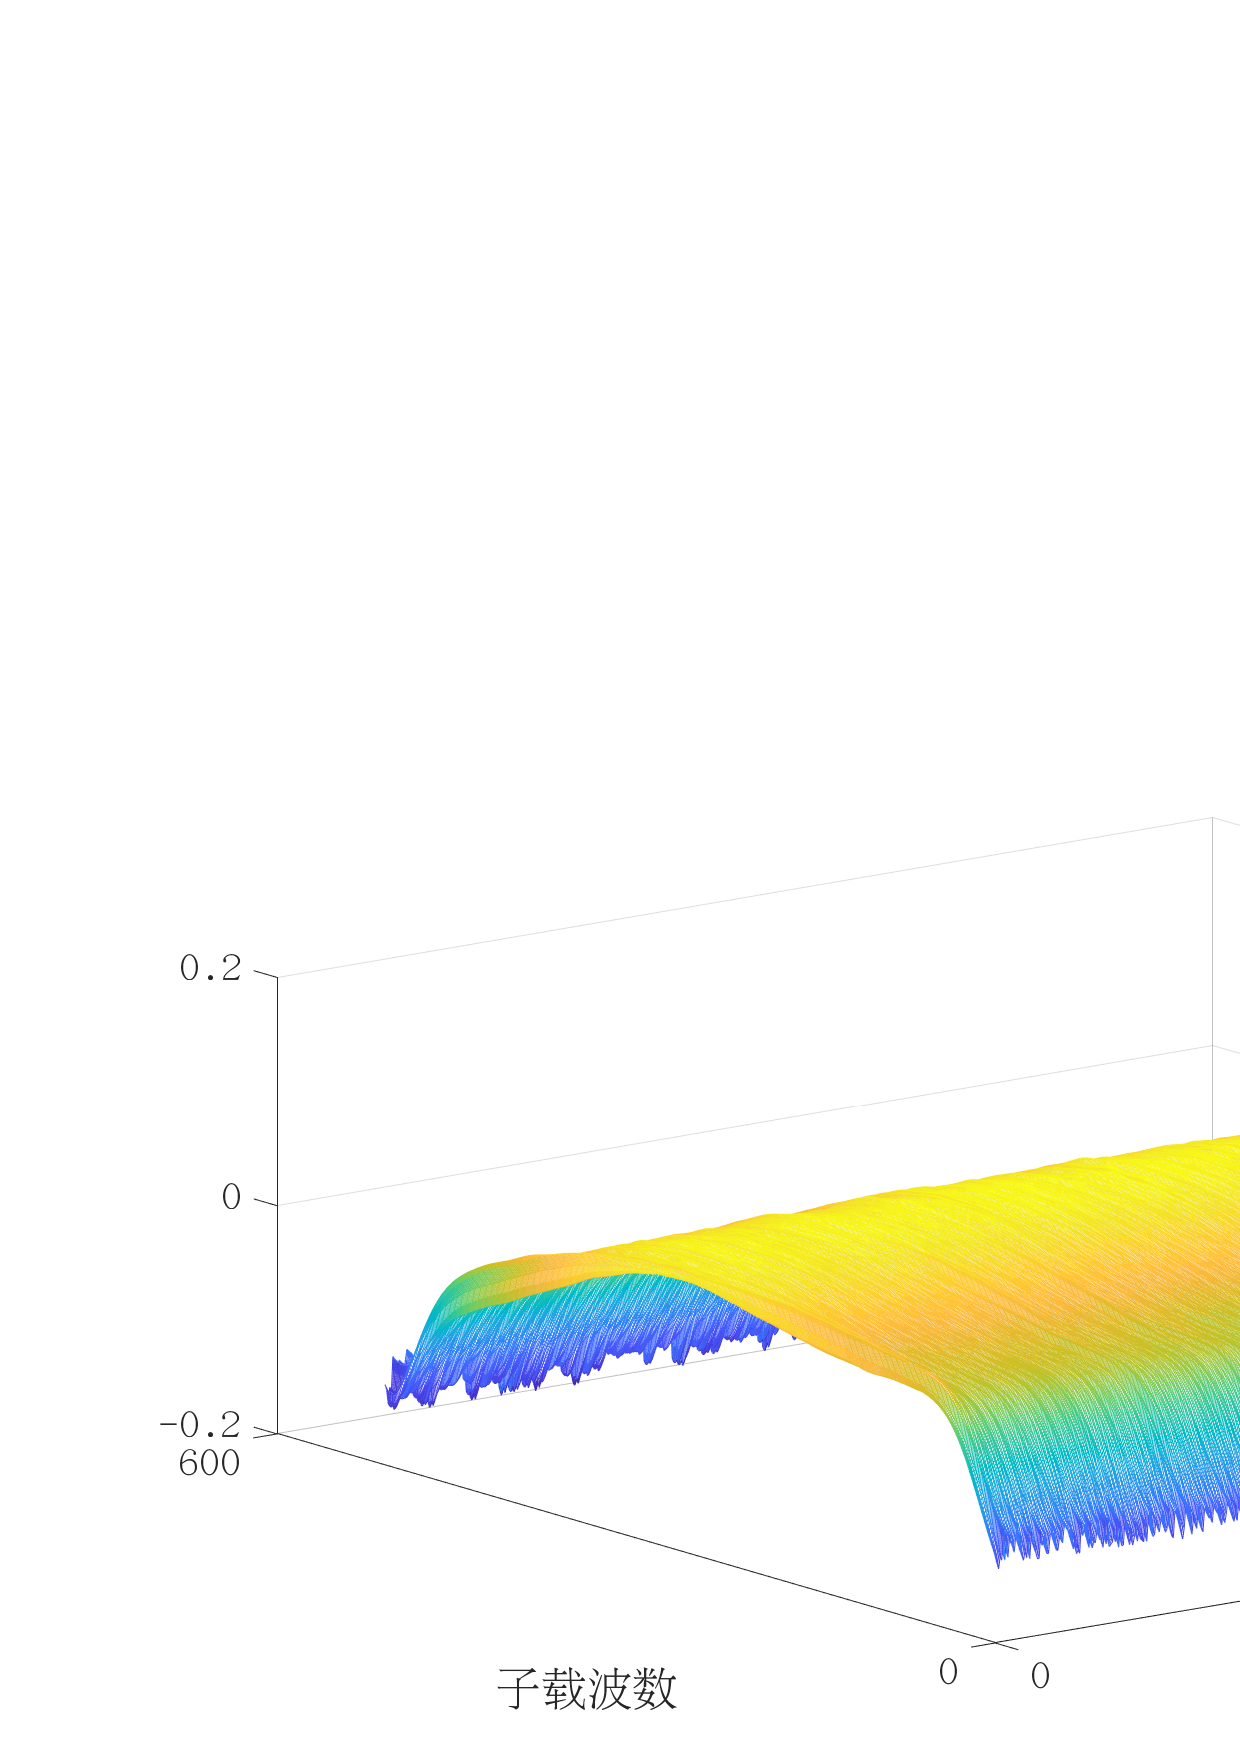
\includegraphics[width=0.3\textwidth]{images/tdd-csi/indoor-no-move.jpg}
    }
    \subfigure[室内-方式2]{
        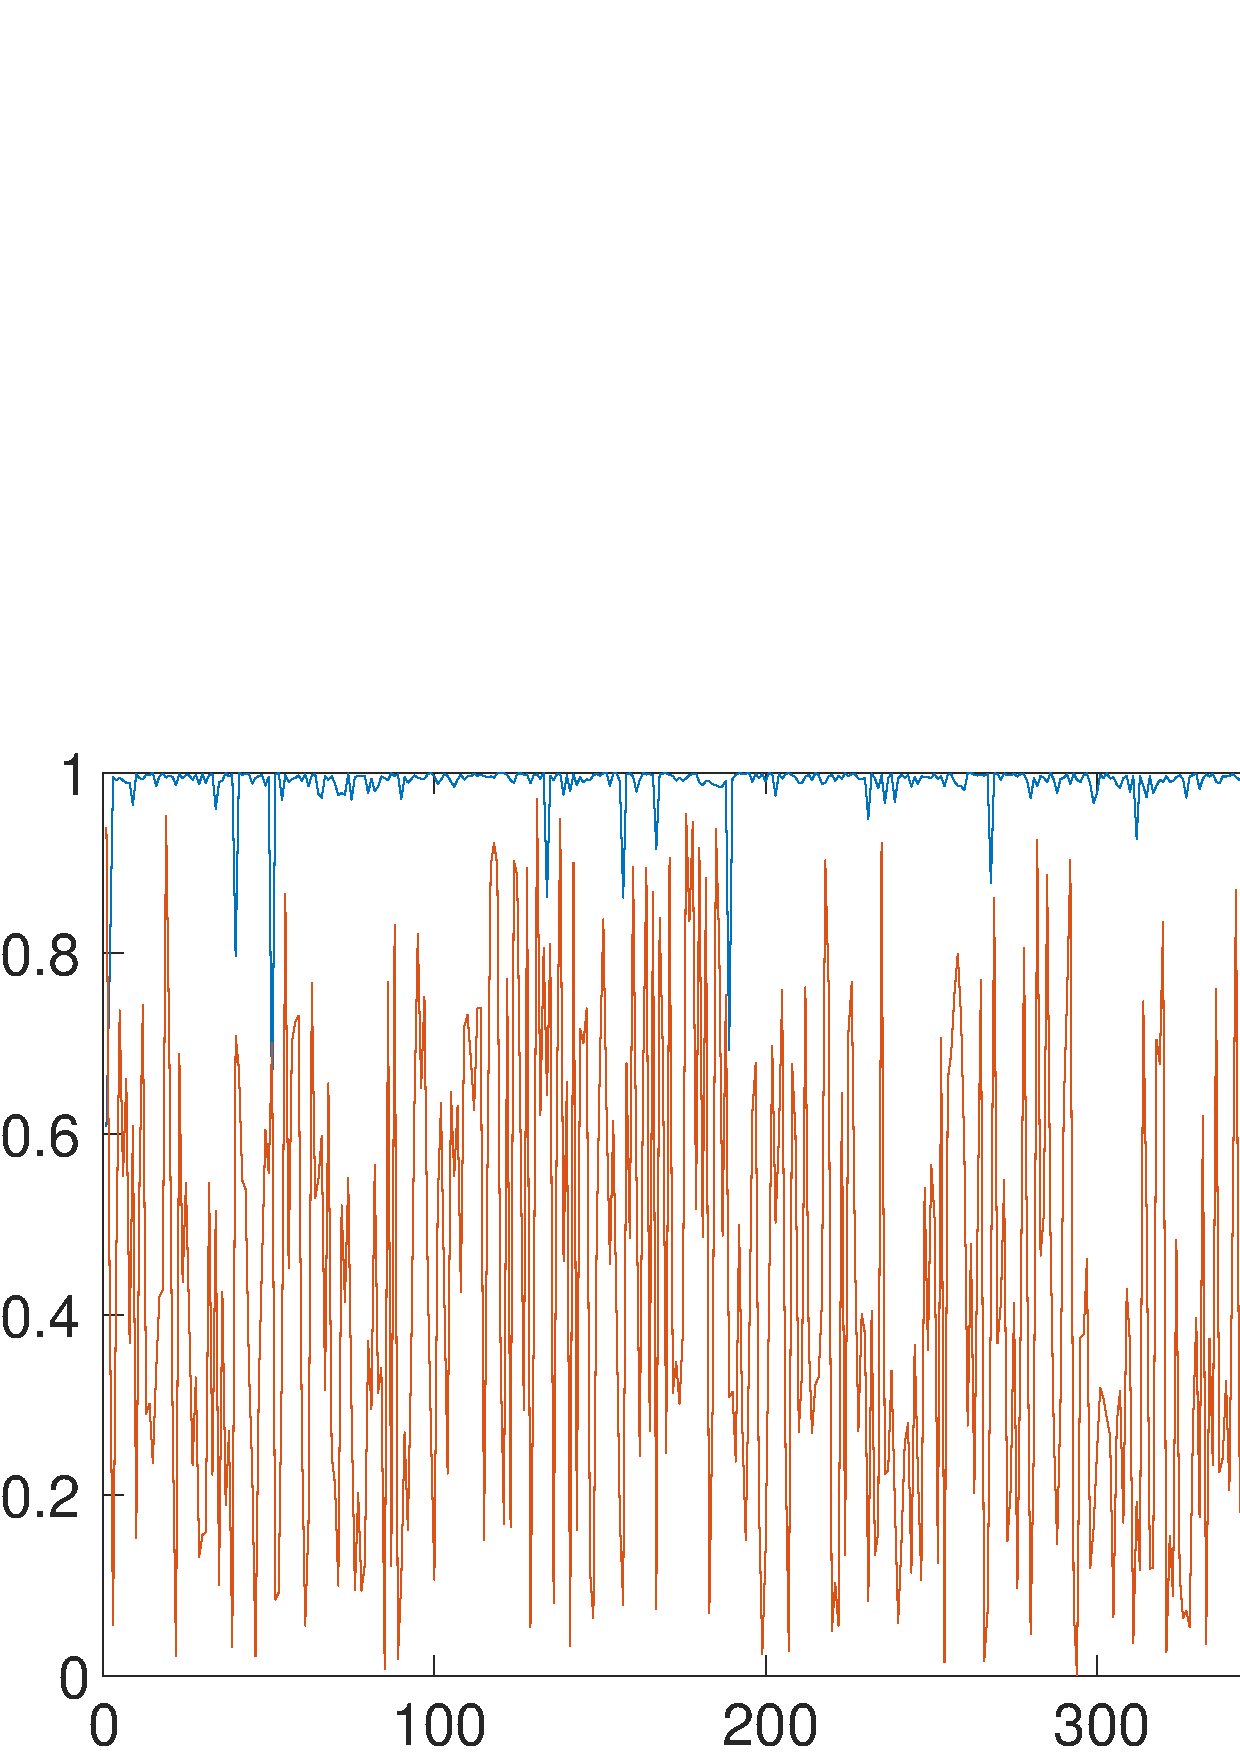
\includegraphics[width=0.3\textwidth]{images/tdd-csi/indoor-people-move.jpg}
    }
    \subfigure[室内-方式3]{
        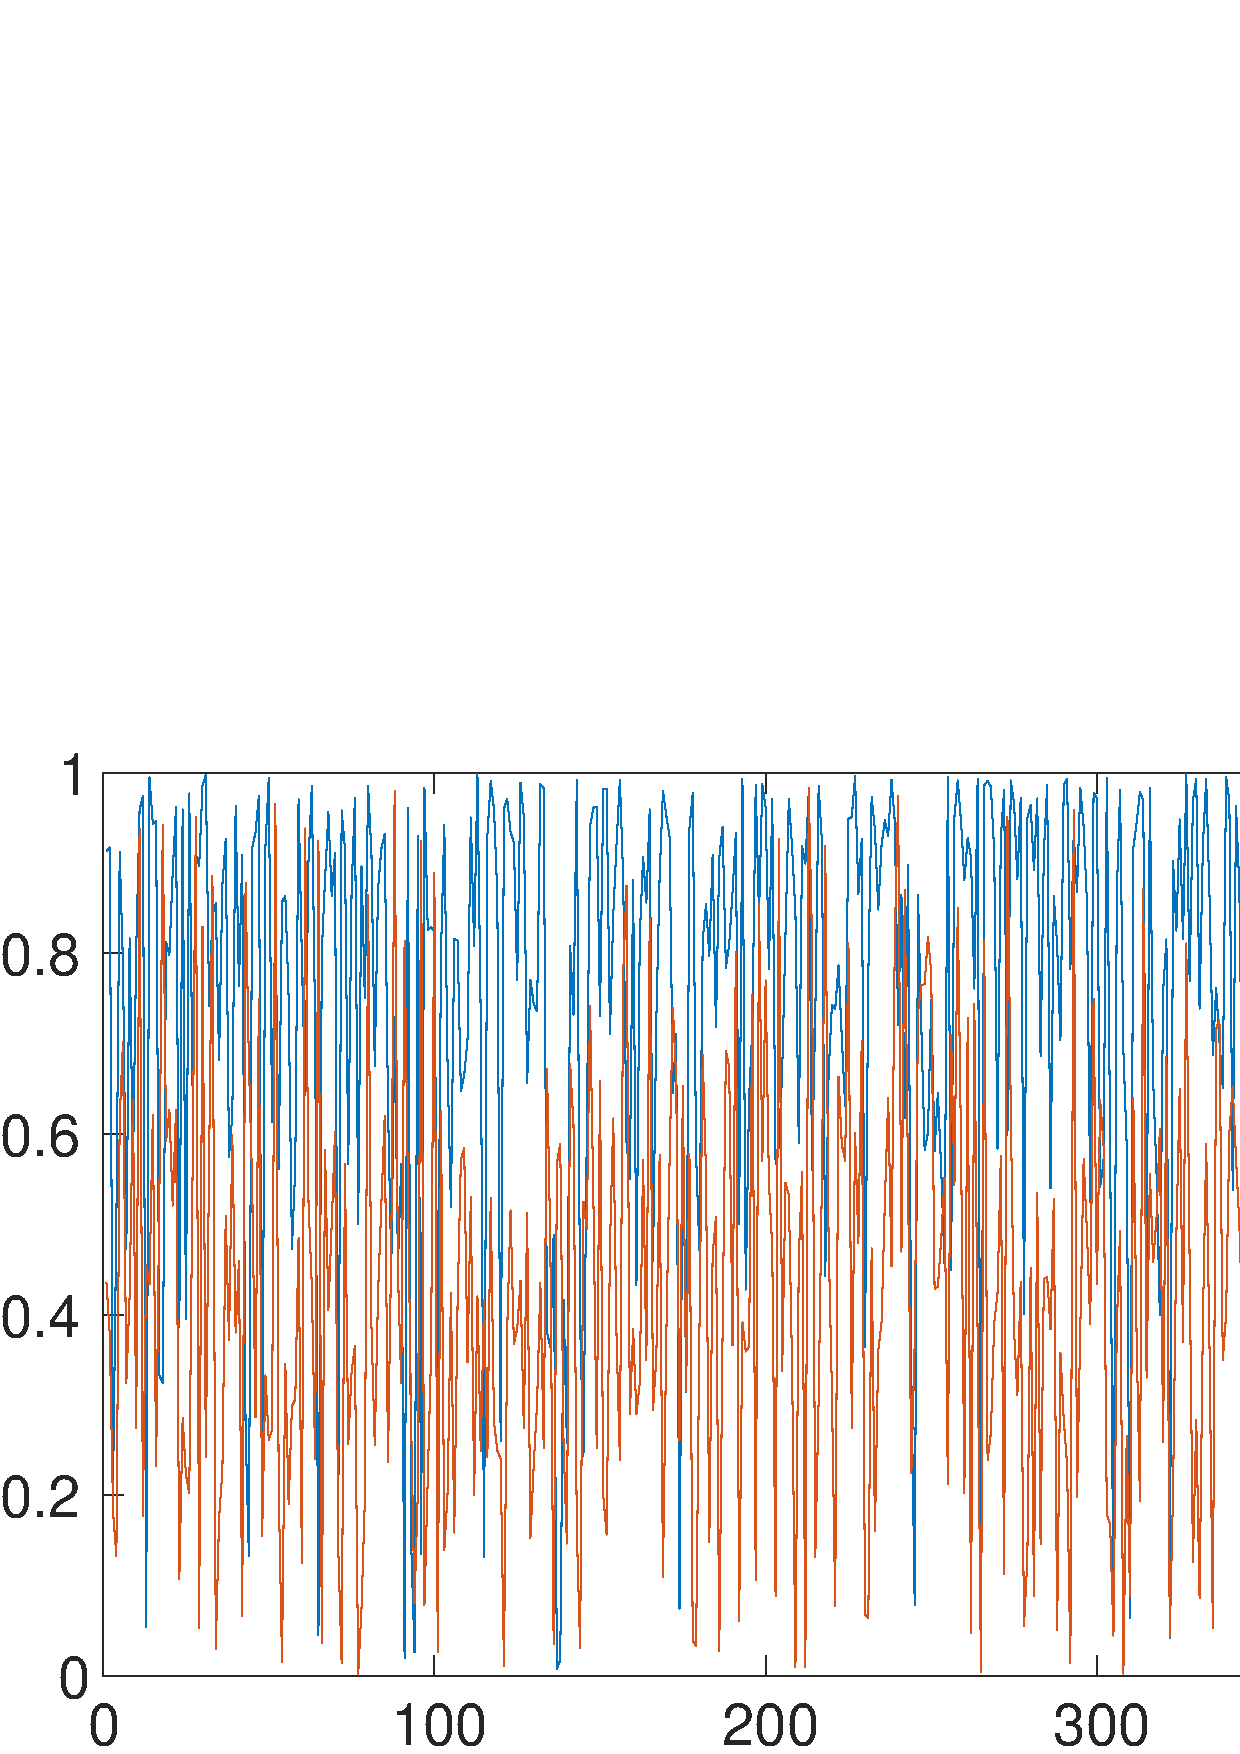
\includegraphics[width=0.3\textwidth]{images/tdd-csi/indoor-trolly-move.jpg}
    }
    \quad    %用 \quad 来换行
    \subfigure[走廊-方式1]{
        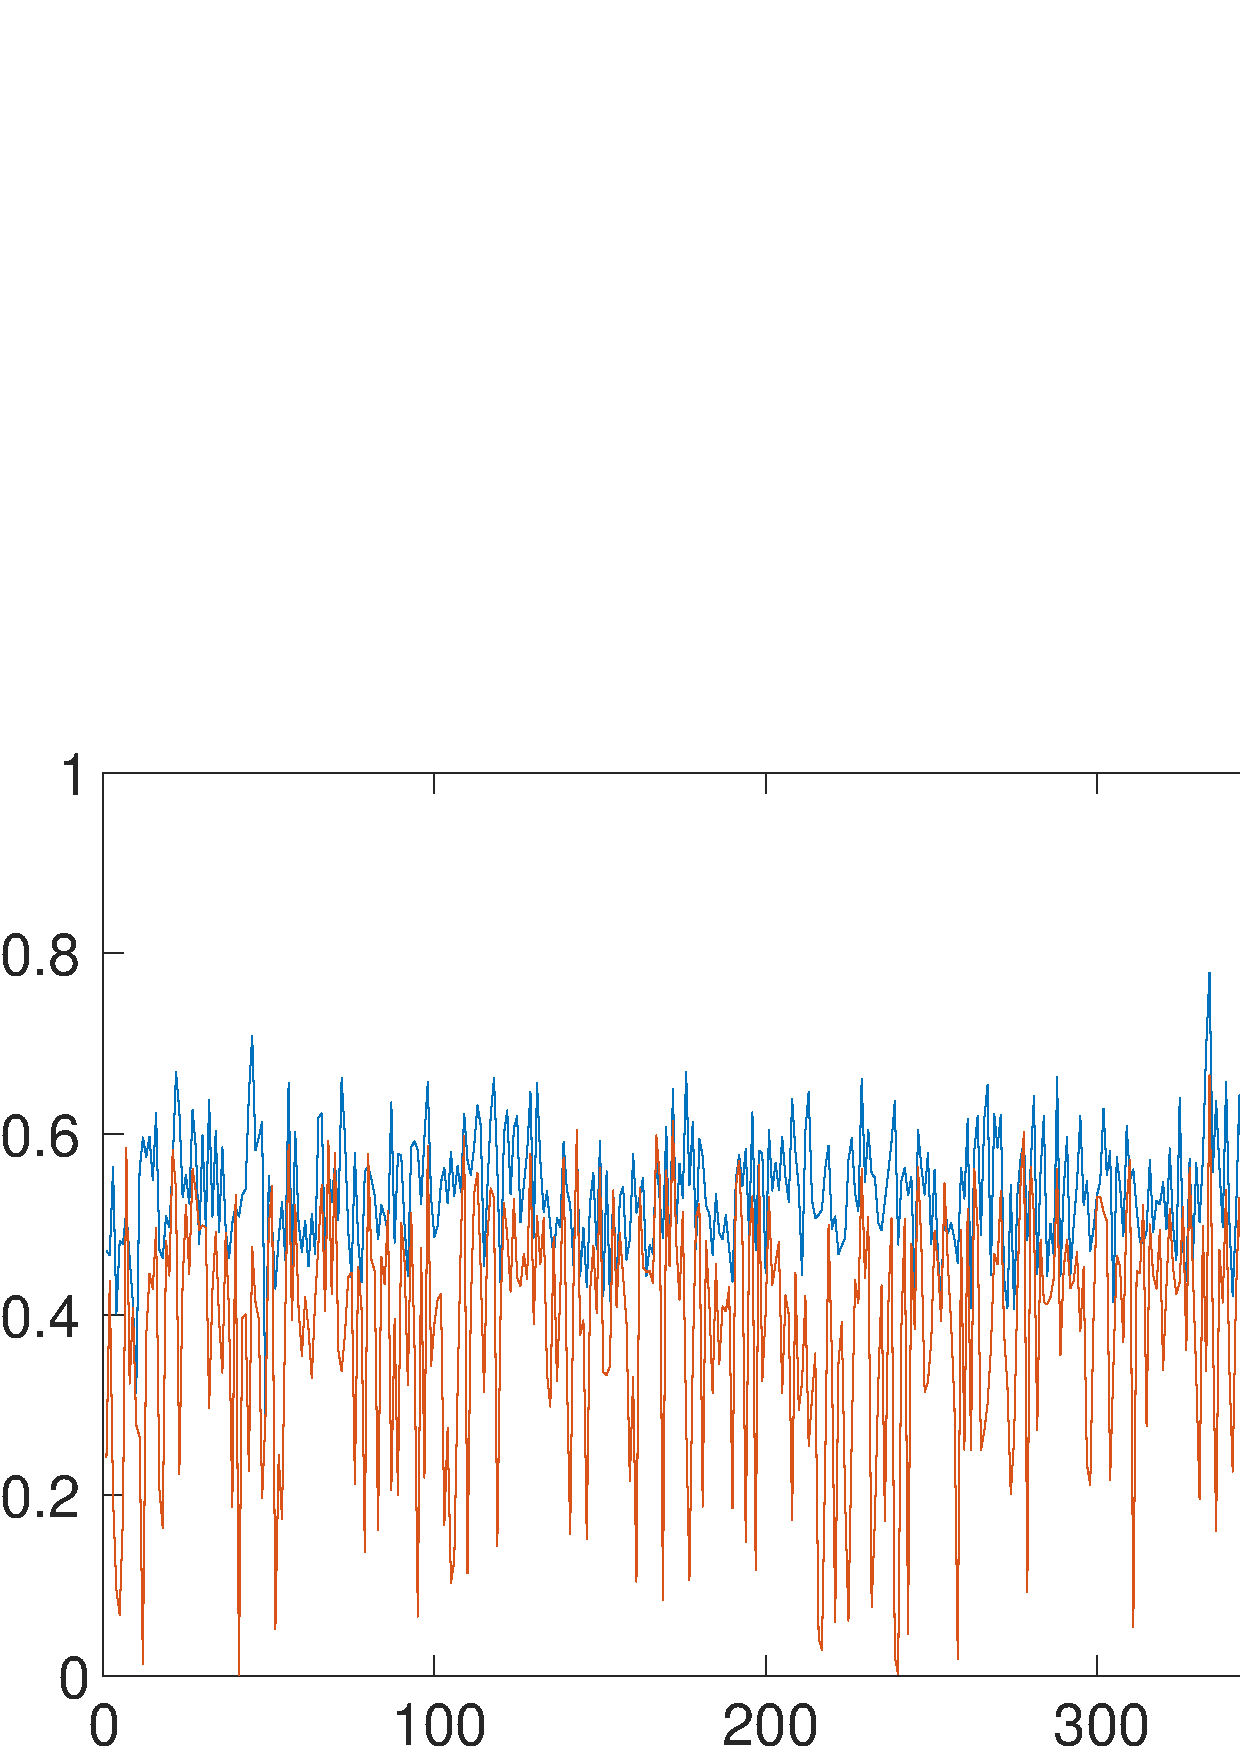
\includegraphics[width=0.3\textwidth]{images/tdd-csi/corridor-no-move.jpg}
    }
    \subfigure[走廊-方式2]{
        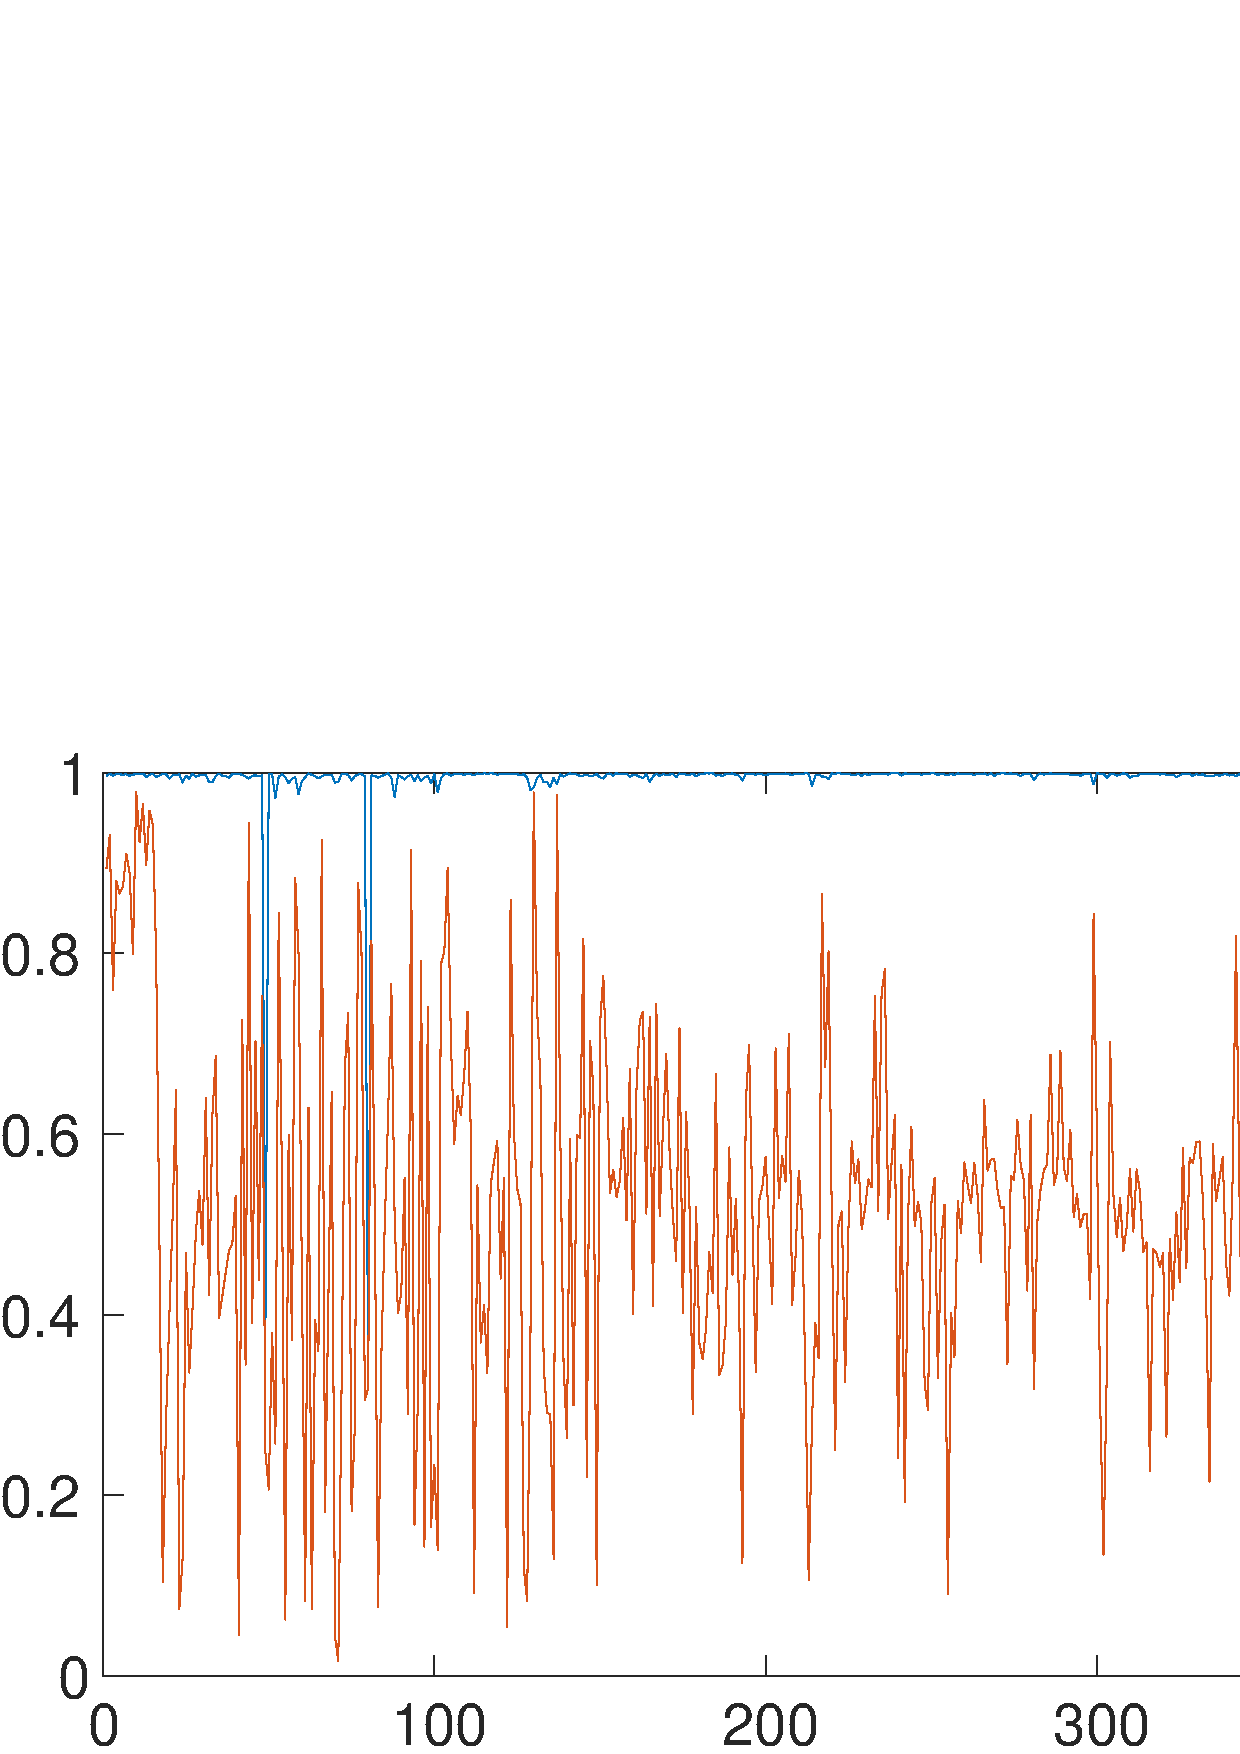
\includegraphics[width=0.3\textwidth]{images/tdd-csi/corridor-people-move.jpg}
    }
    \subfigure[走廊-方式3]{
        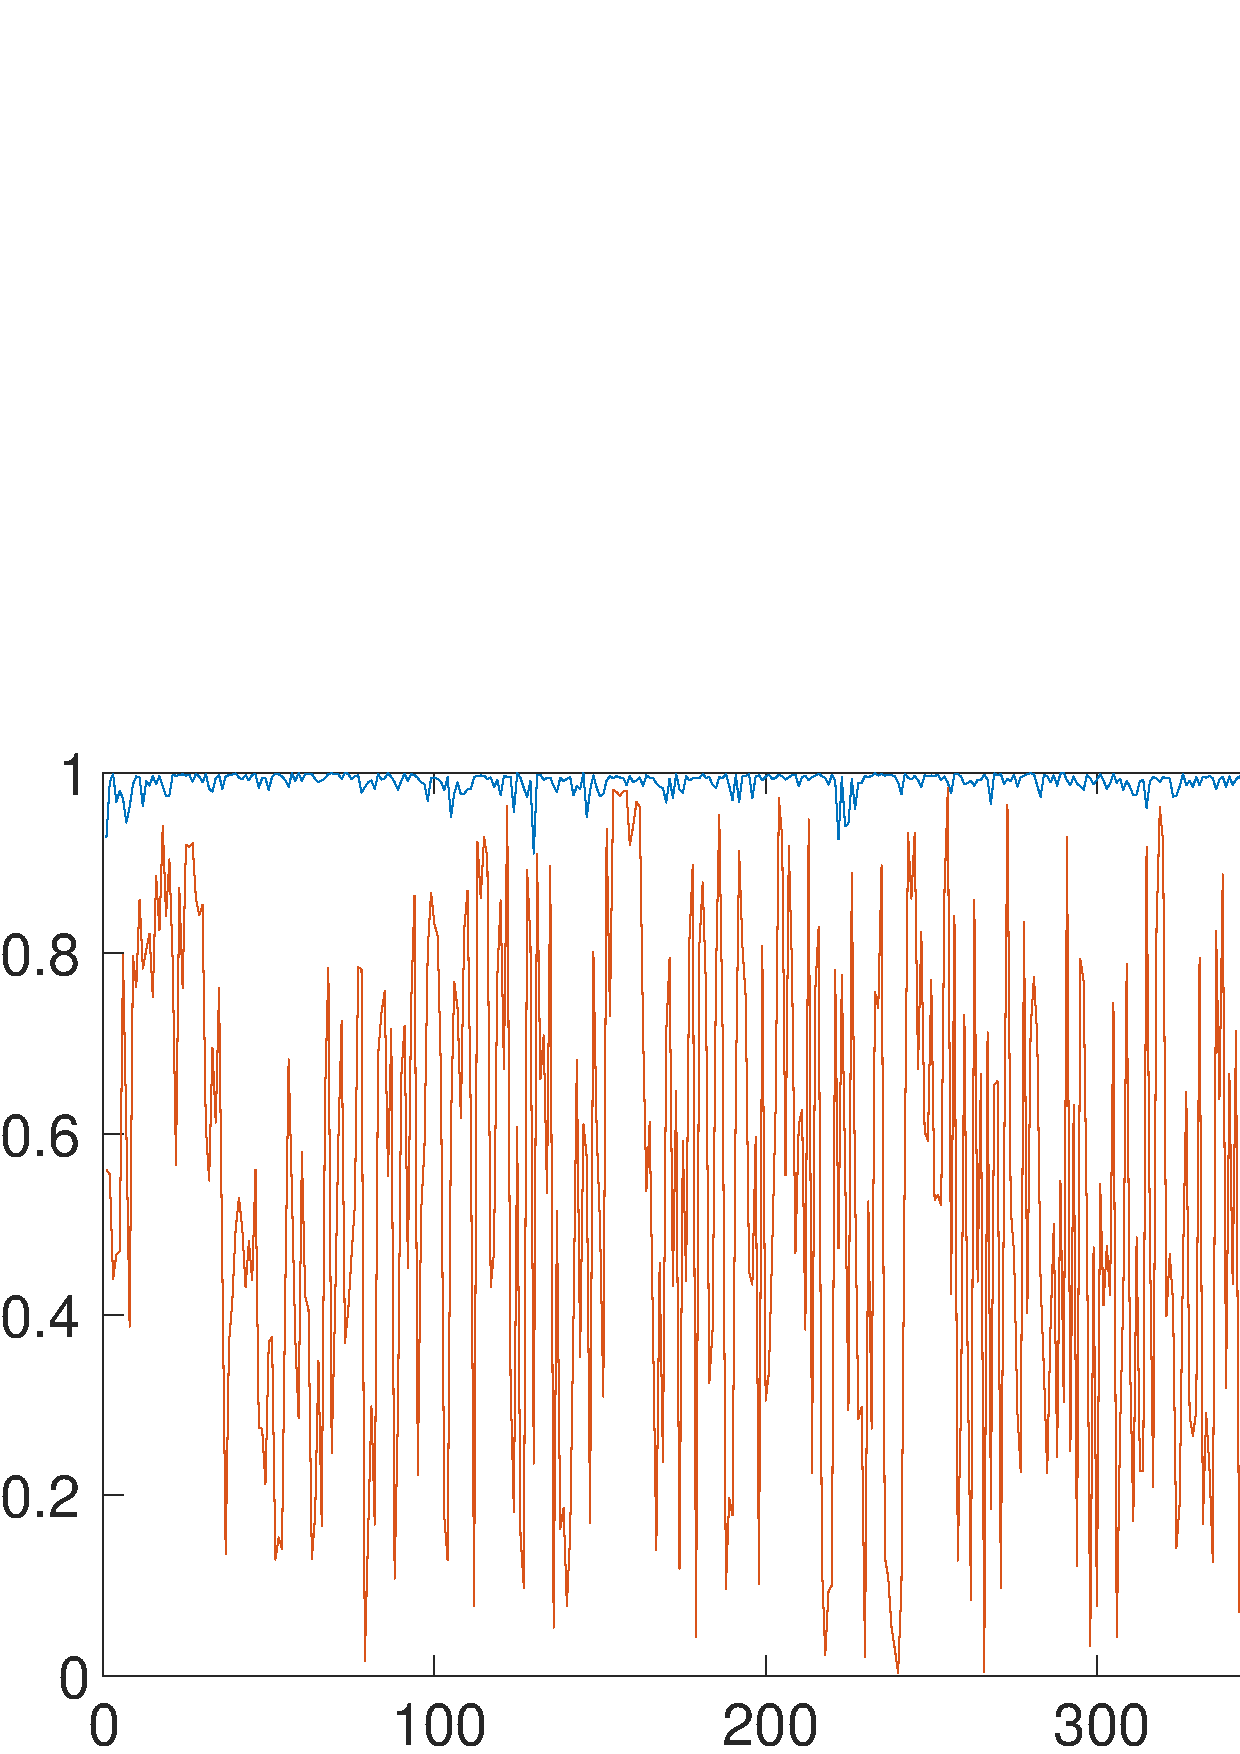
\includegraphics[width=0.3\textwidth]{images/tdd-csi/corridor-trolly-move.jpg}
    }
    \quad
    \subfigure[室外-方式1]{
        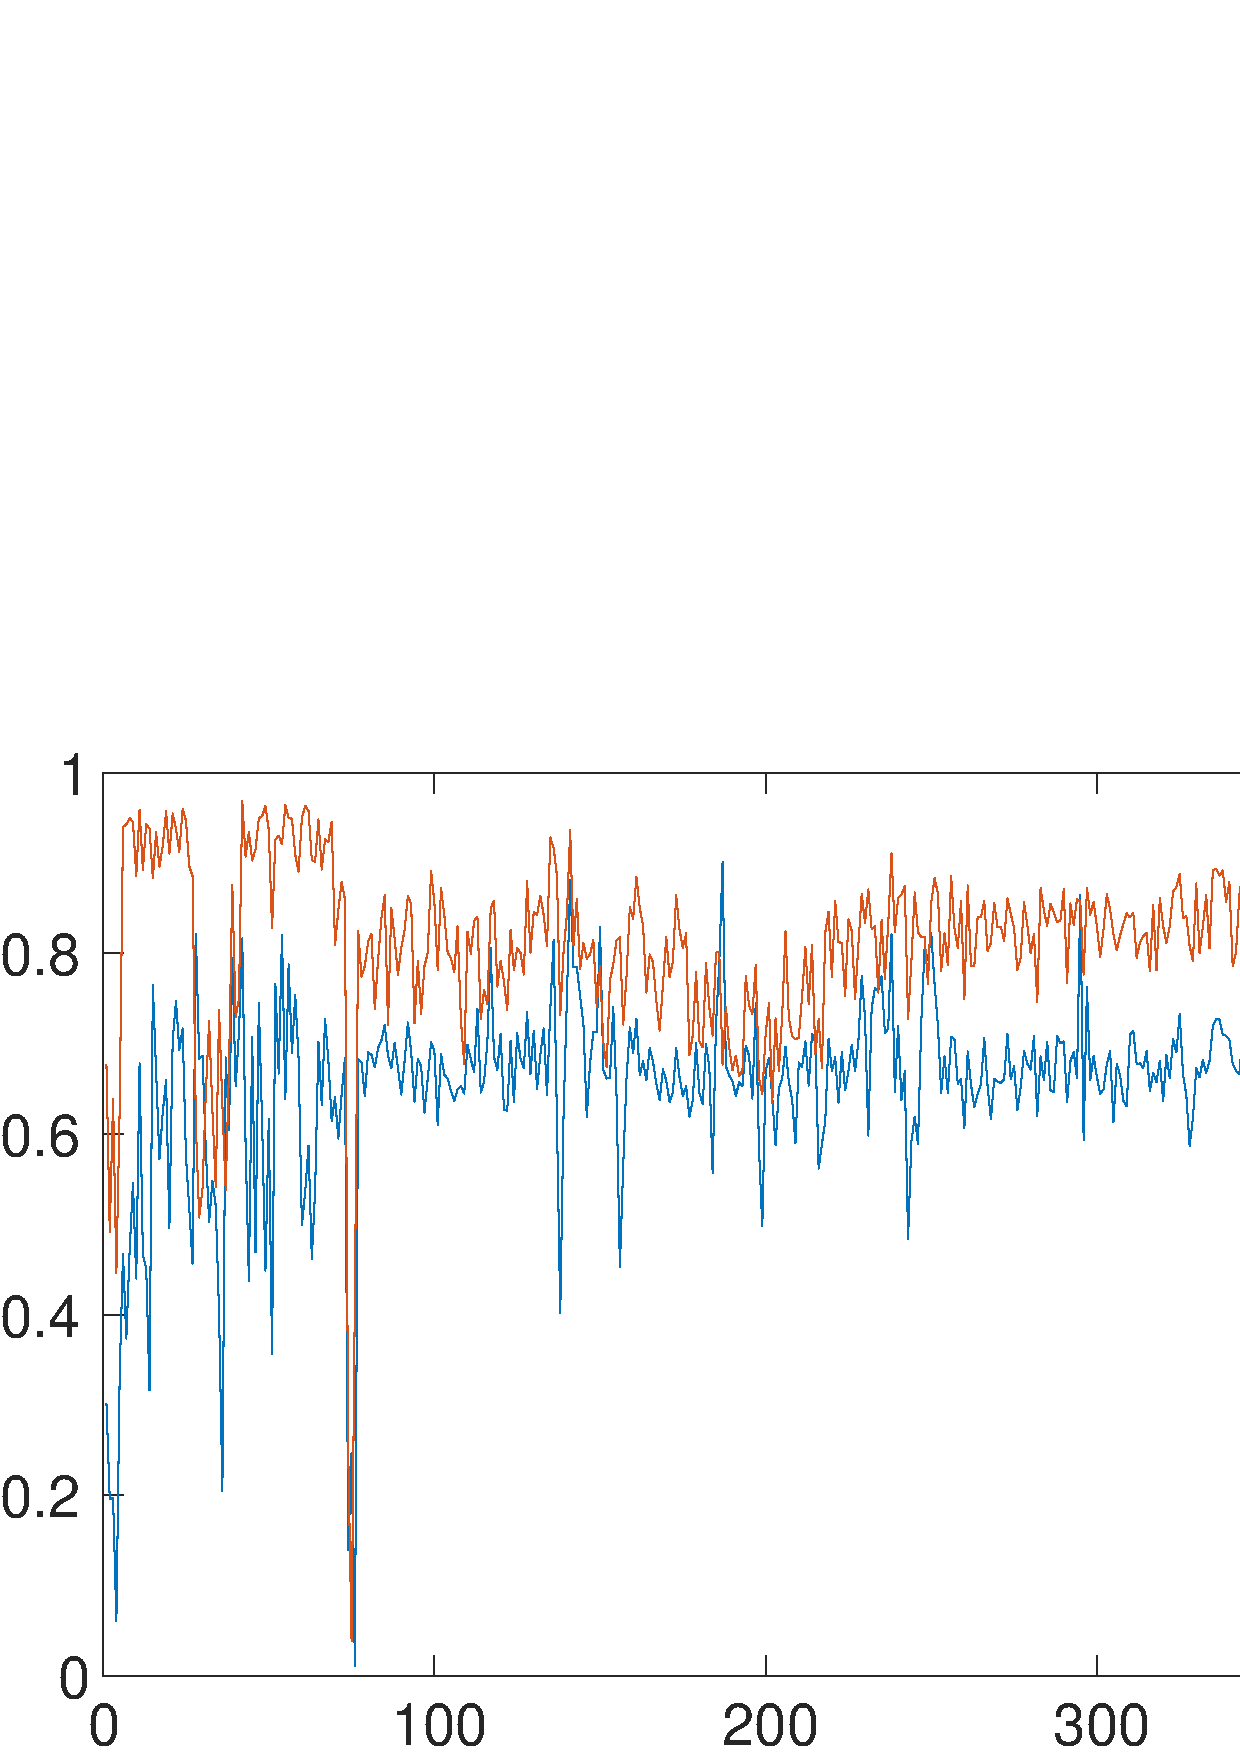
\includegraphics[width=0.3\textwidth]{images/tdd-csi/outdoor-no-move.jpg}
    }
    \subfigure[室外-方式2]{
        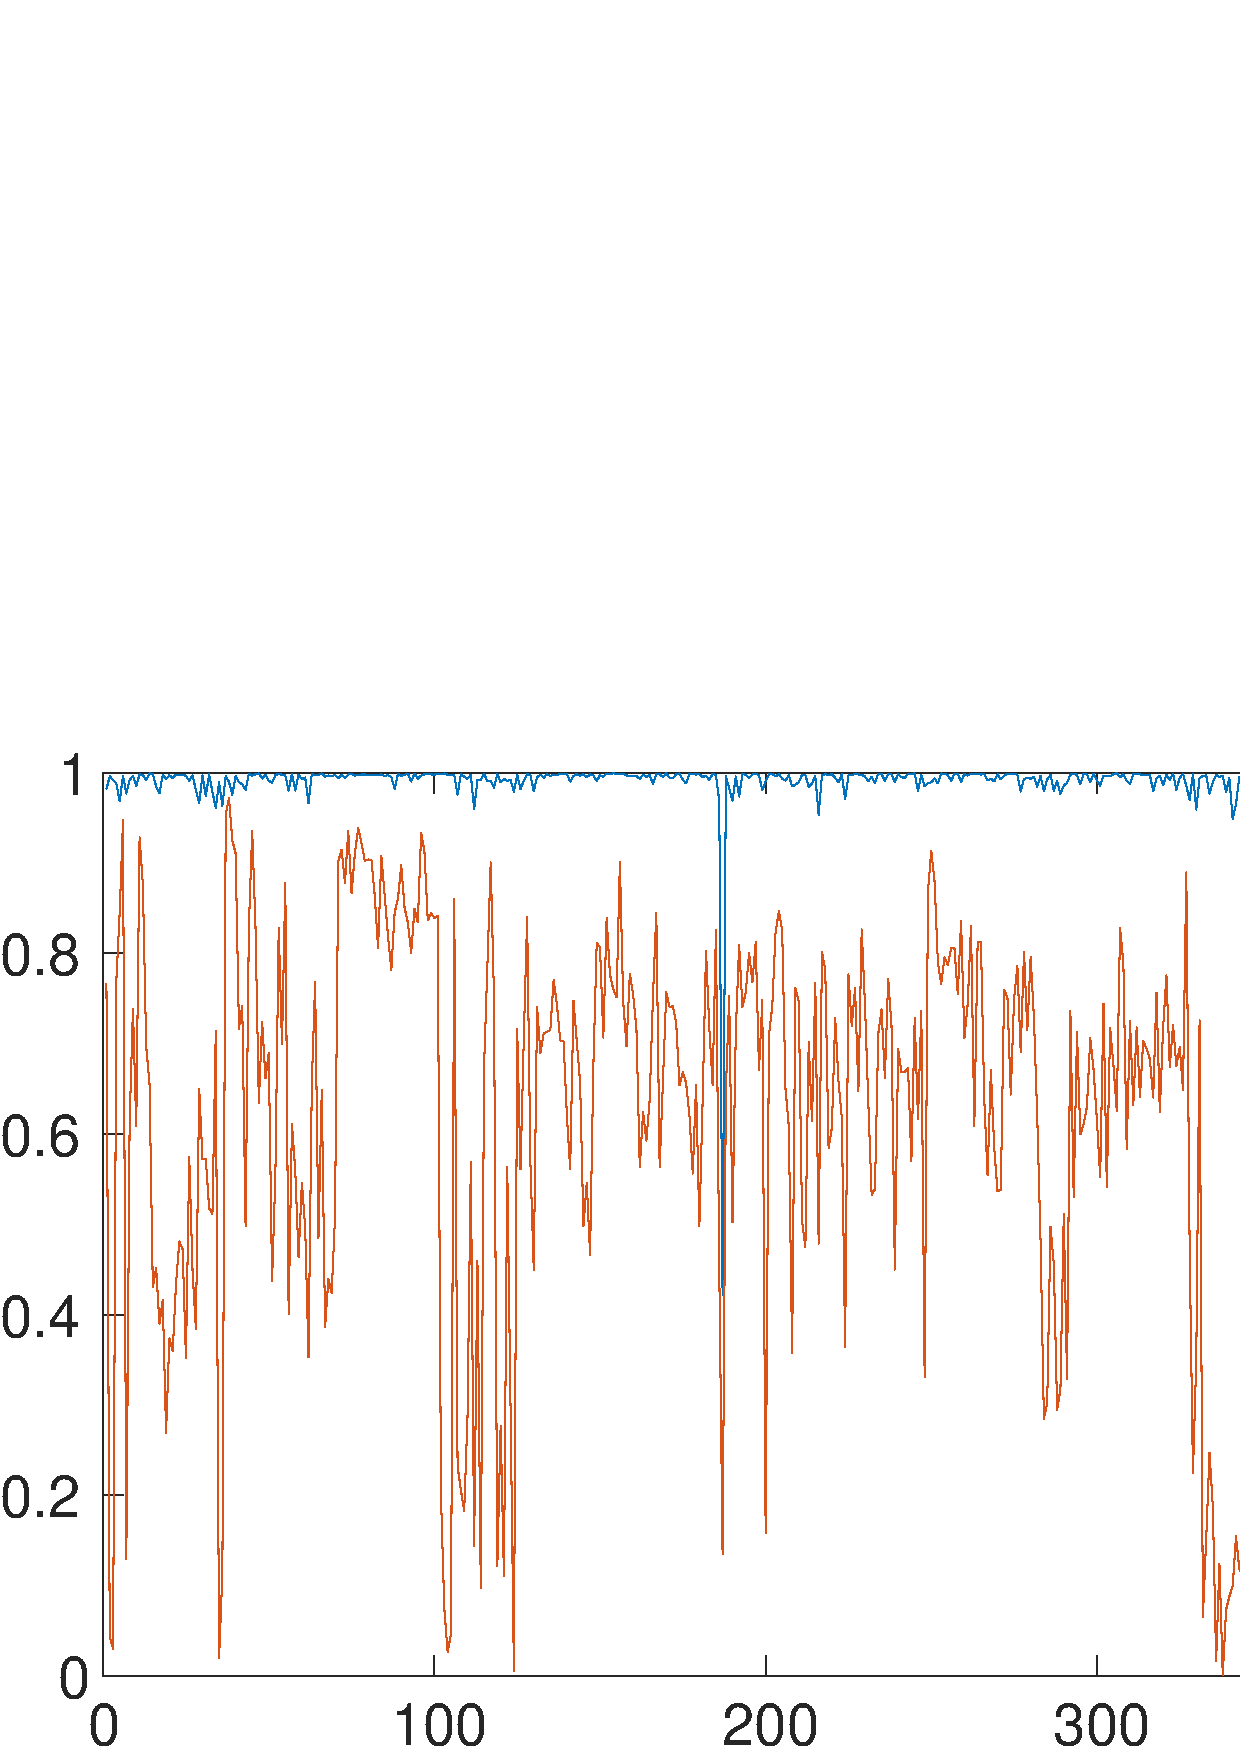
\includegraphics[width=0.3\textwidth]{images/tdd-csi/outdoor-people-move.jpg}
    }
    \subfigure[室外-方式3]{
        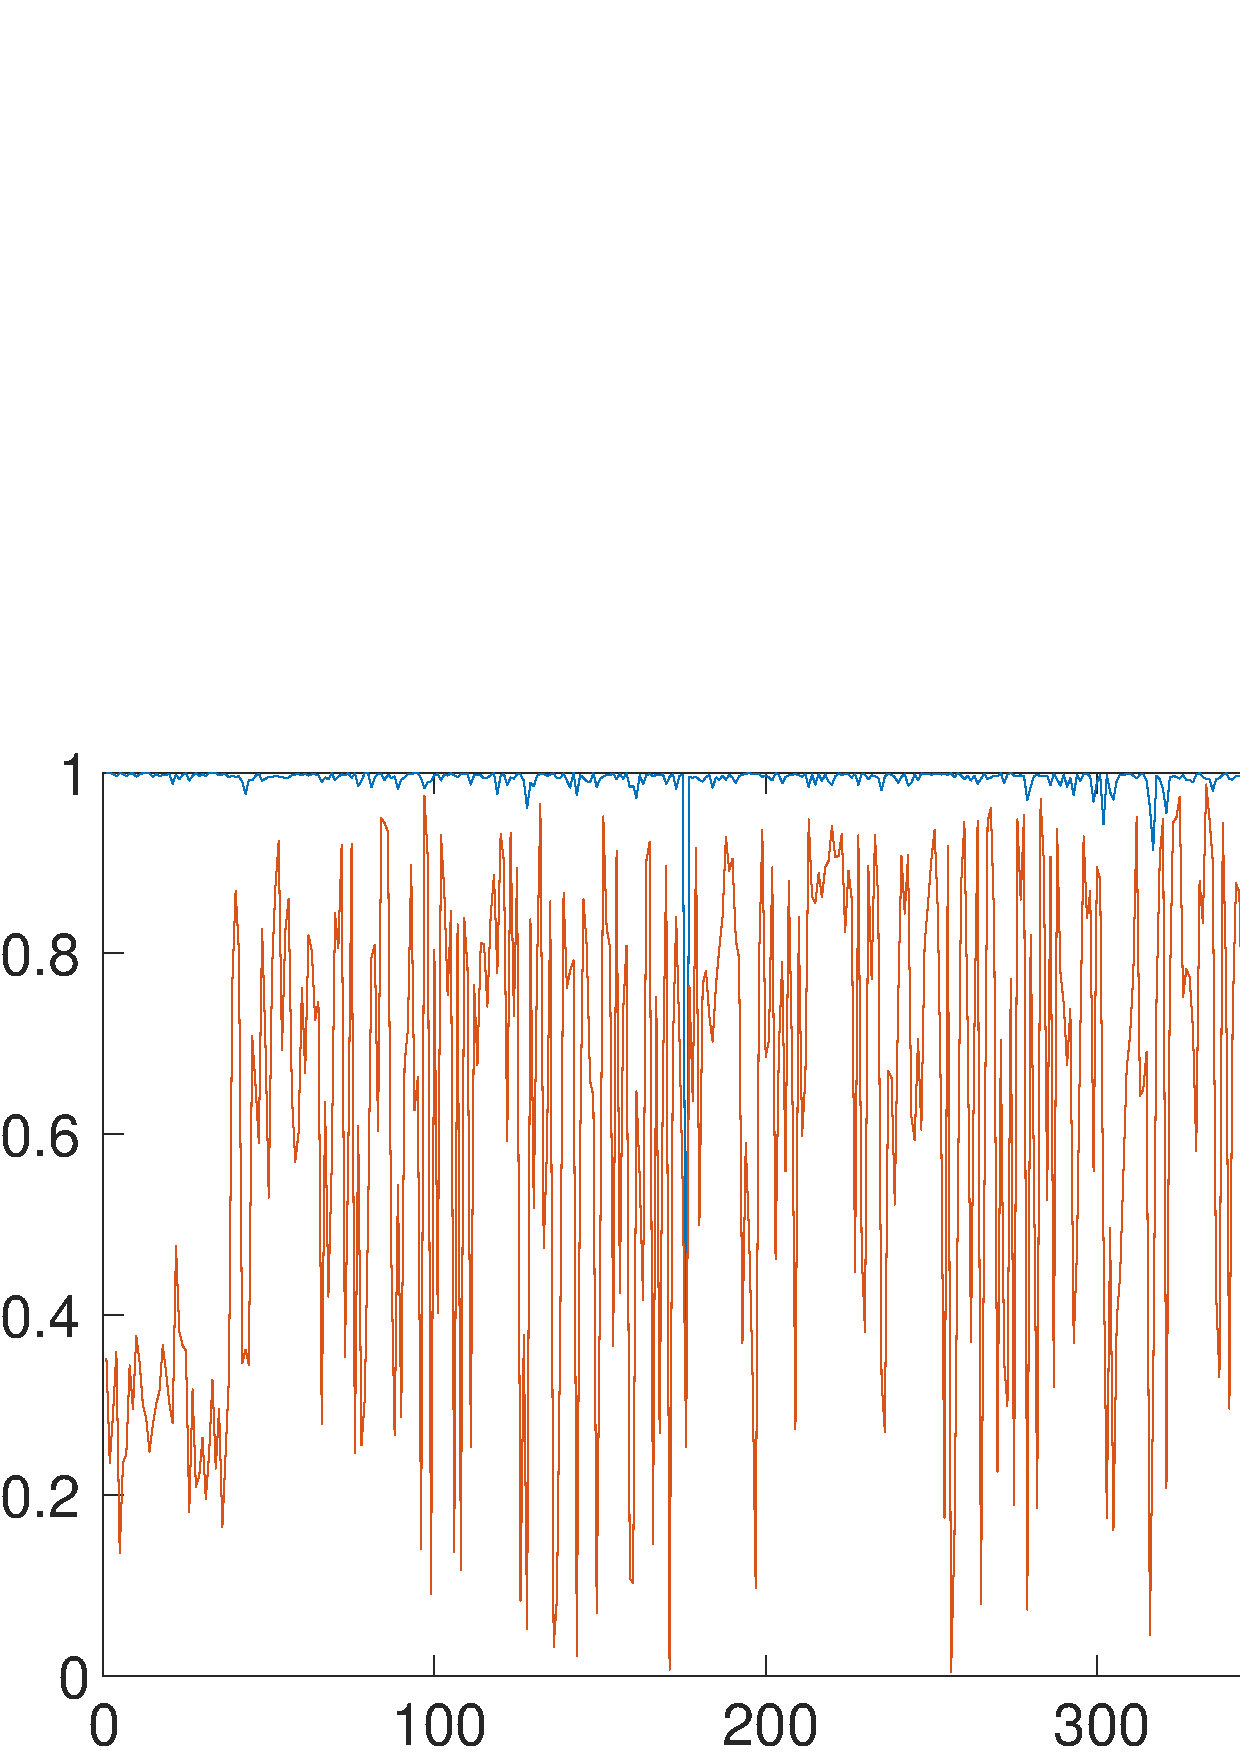
\includegraphics[width=0.3\textwidth]{images/tdd-csi/outdoor-trolly-move.jpg}
    }
    \caption{不同场景与环境下CSI结果展示}{} % xcorr between alice and bob, xcorr between bob and eve
    \label{tdd_csi_ab}
\end{figure}

% Please add the following required packages to your document preamble:
% \usepackage{multirow}
\begin{table}[]
    \centering
    \begin{tabular}{|l|l|l|l|}
    \hline
    \multicolumn{2}{|c|}{参数} & Alice & Bob \\ \hline
    \multirow{5}{*}{USRP} & 上下行载波频率(MHz) & 2535 & 2535 \\ \cline{2-4} 
     & 采样率(MHz) & 25 & 25 \\ \cline{2-4} 
     & 增益(dB) & 30 & 30 \\ \cline{2-4} 
     & 天线 & Tx/Rx & Tx/Rx \\ \cline{2-4} 
     & 带宽(MHz) & 20 & 20 \\ \hline
    \multirow{4}{*}{导频信号} & 正弦波长度 & 1504 & 1504 \\ \cline{2-4} 
     & 正弦波频率(Hz) & 4 & 8 \\ \cline{2-4} 
     & M序列长度 & 4095 & 4095 \\ \cline{2-4} 
     & CP循环前缀长度 & 129 & 129 \\ \hline
    \end{tabular}
    \caption{TDD模式下的实验参数
    \label{tdd-exp-args}}
\end{table}

\subsection{CSI相关性}

本文对每一组数据使用公式(\ref{equation_corr_ab})和公式(\ref{equation_corr_ae})分别计算Alice和Bob之间CSI的皮尔逊相关系数、Alice和Eve之间CSI的皮尔逊相关系数。在9种情况下,计算600组数据,得到图\ref{tdd_csi_xcorr}。其中蓝色表示Alice和Bob之间CSI的皮尔逊相关系数,红色表示Alice和Eve之间CSI的皮尔逊相关系数。可以看到Alice和Bob之间CSI的相关系数稳定在1附近,Alice和Eve之间CSI的相关系数波动较大并且较小。

\begin{figure}
    \centering
    \subfigure[室内-方式1]{
        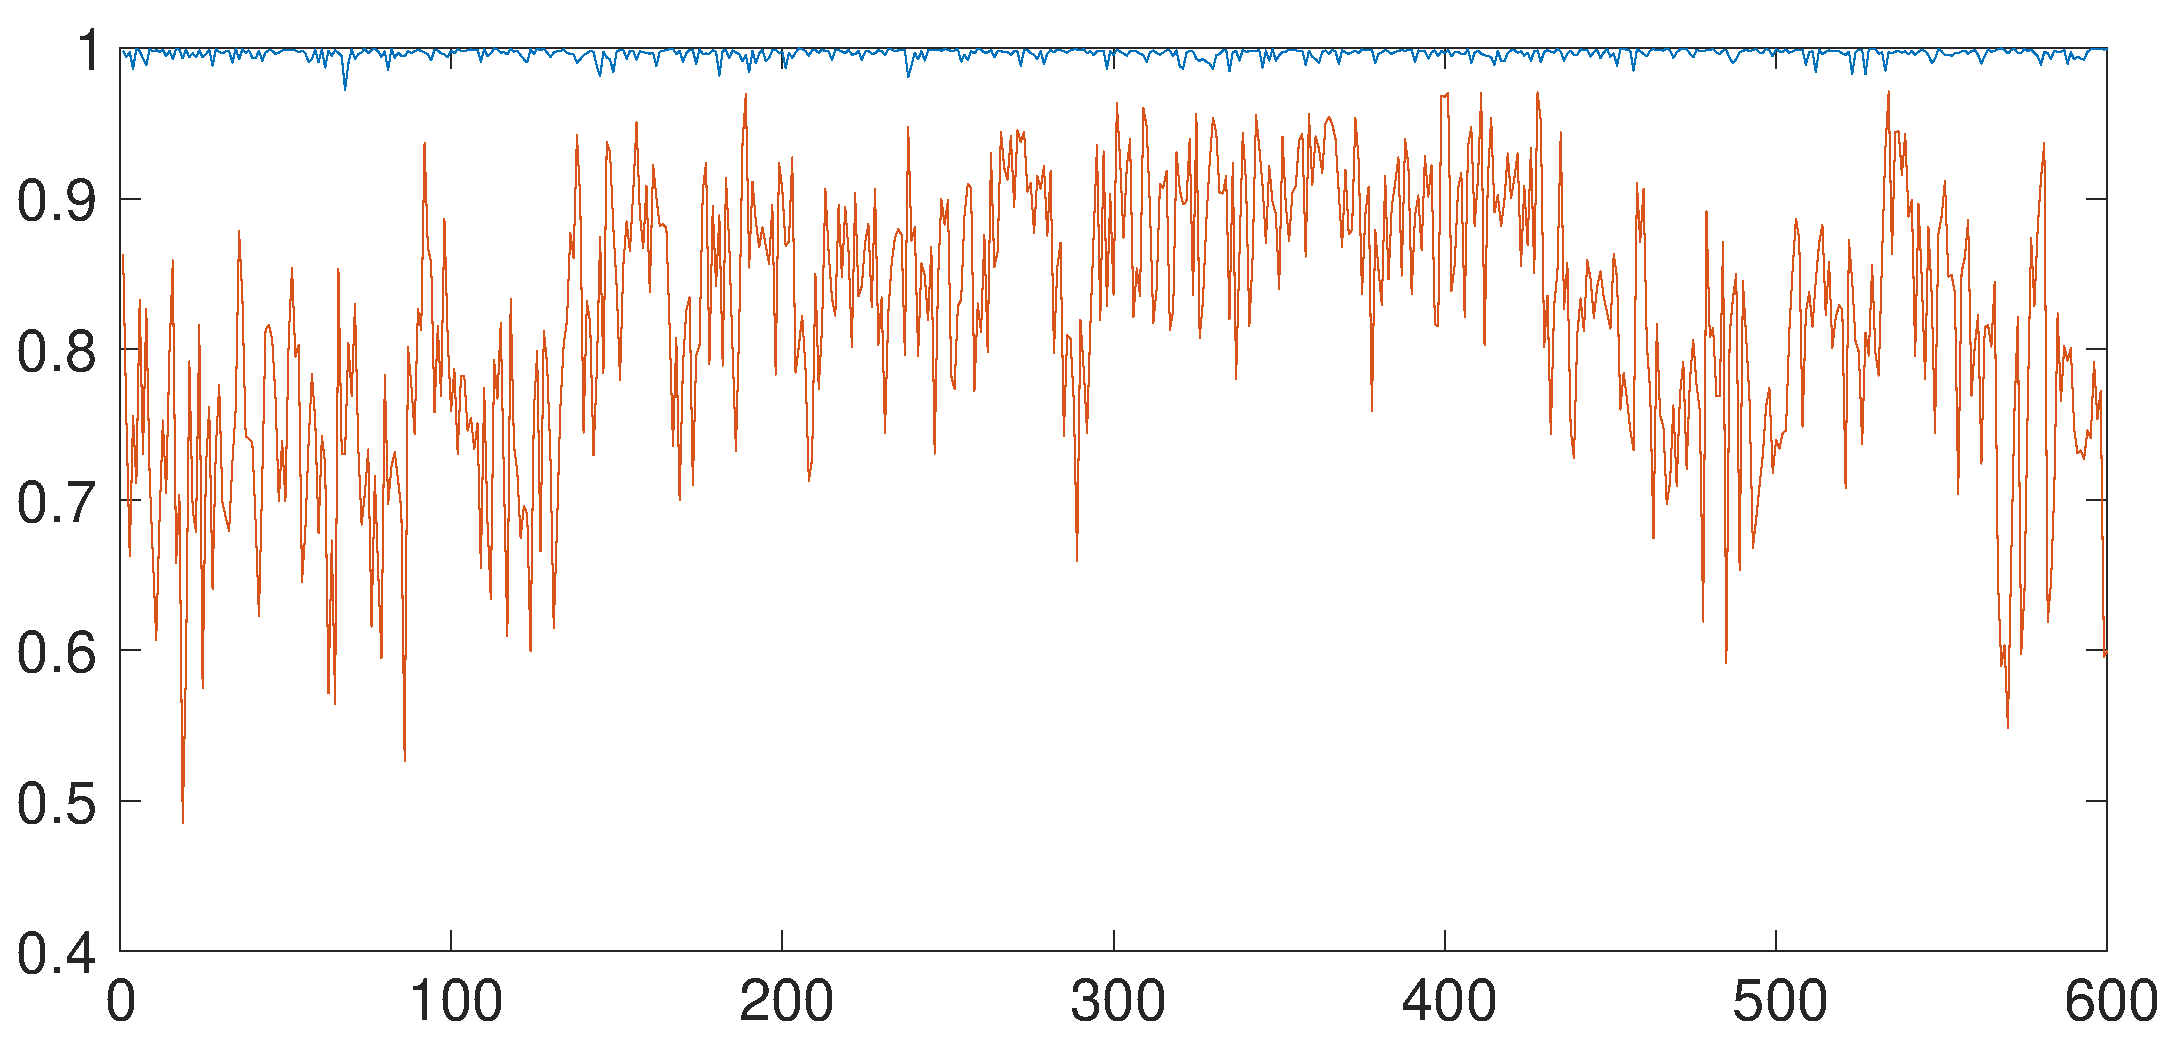
\includegraphics[width=0.3\textwidth]{images/tdd-xcorr/indoor-no-move.eps}
    }
    \subfigure[室内-方式2]{
        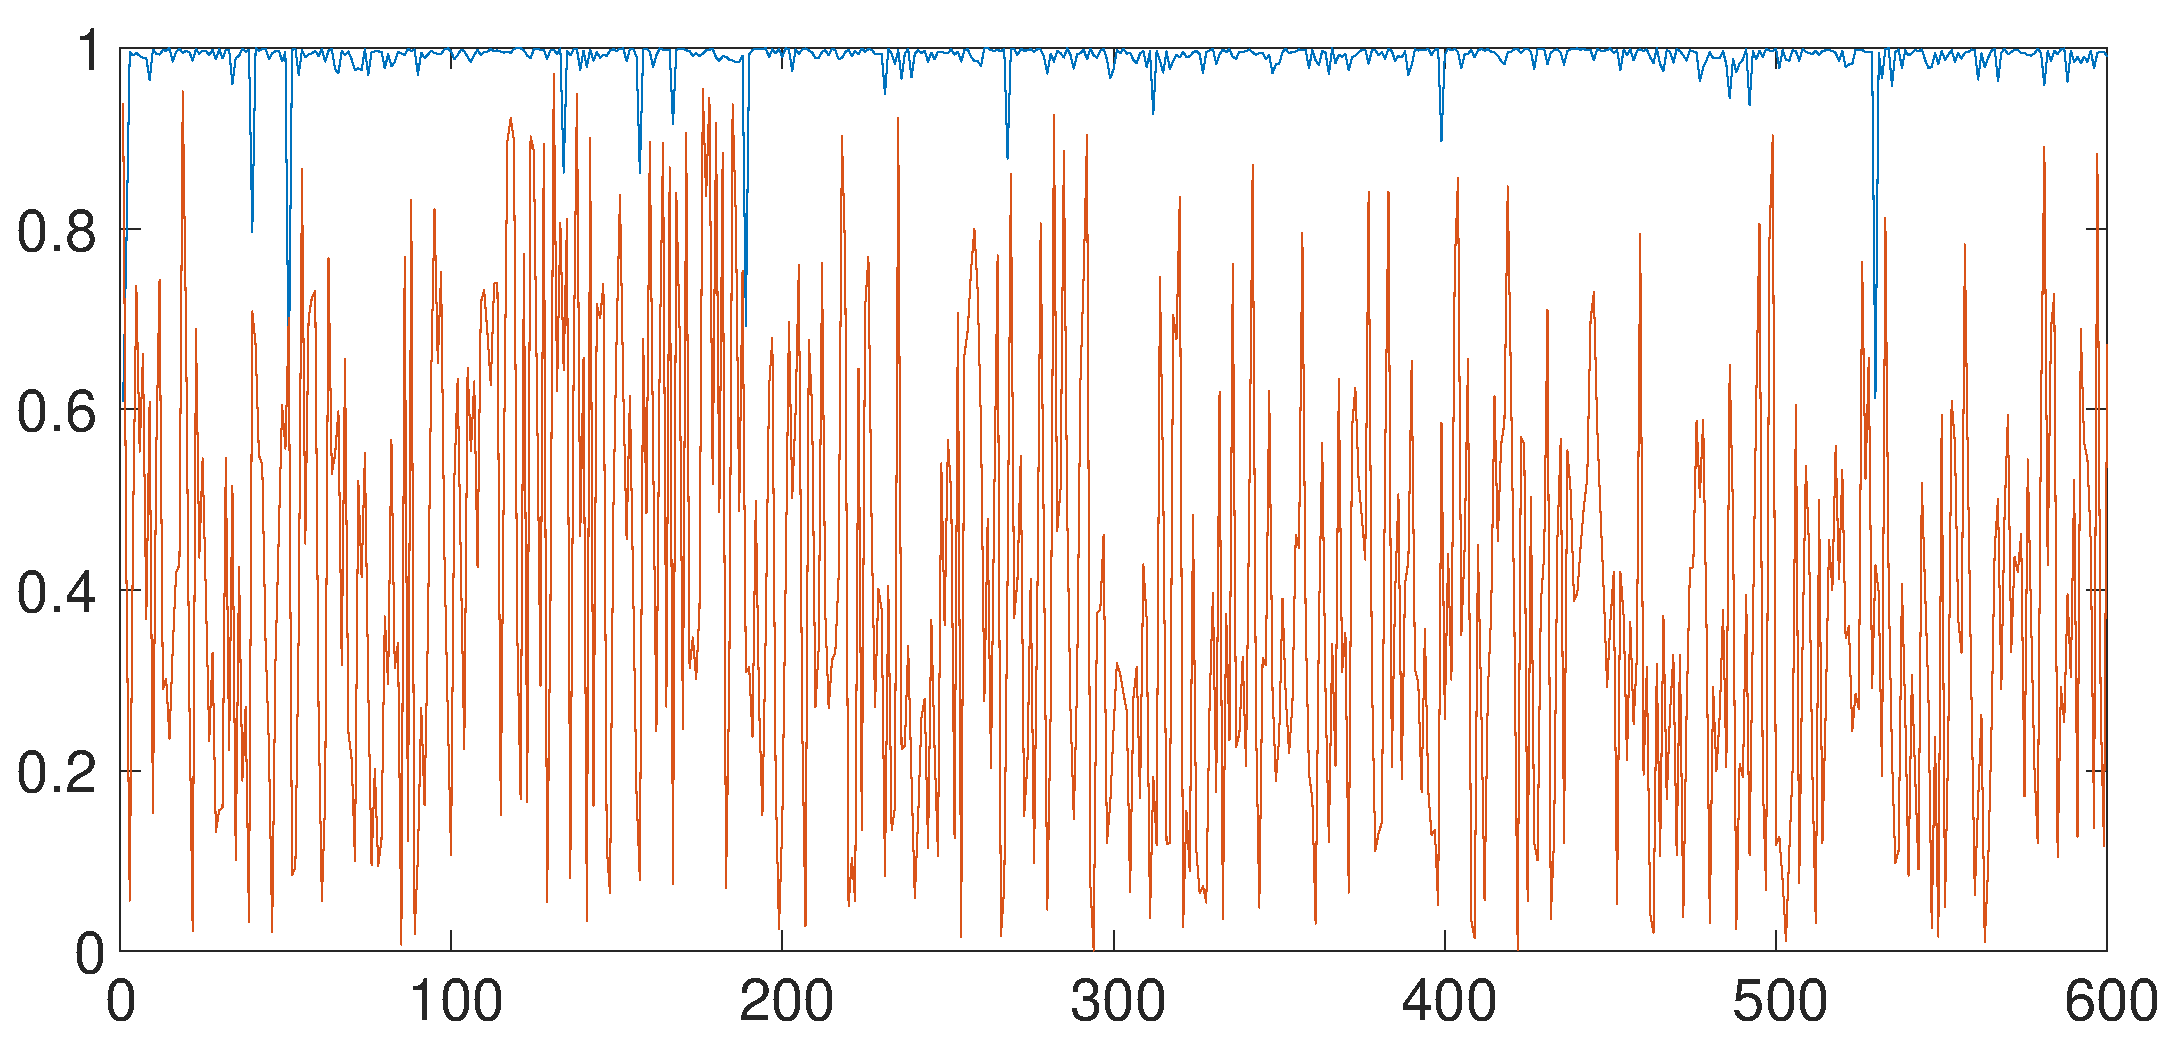
\includegraphics[width=0.3\textwidth]{images/tdd-xcorr/indoor-people-move.eps}
    }
    \subfigure[室内-方式3]{
        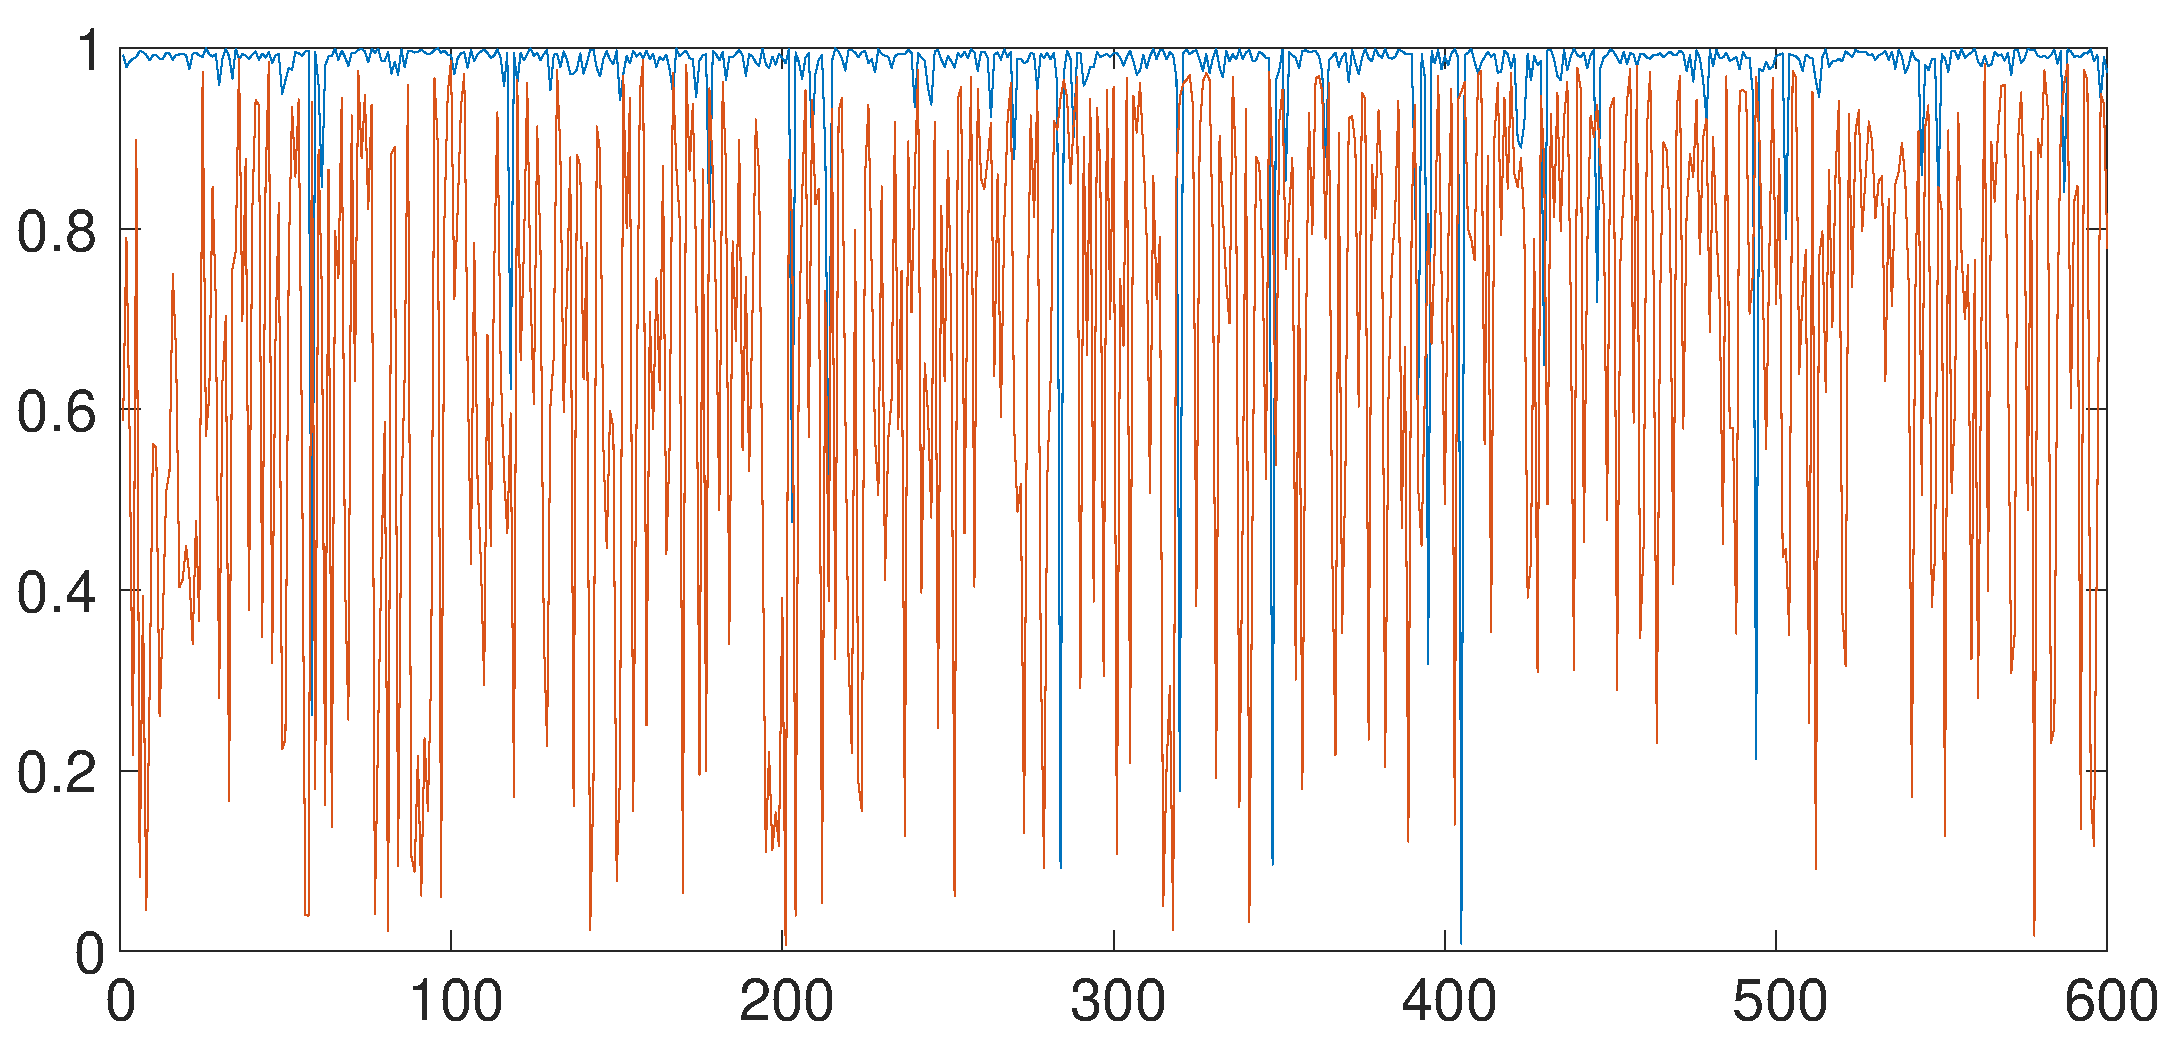
\includegraphics[width=0.3\textwidth]{images/tdd-xcorr/indoor-trolly-move.eps}
    }
    \quad    %用 \quad 来换行
    \subfigure[走廊-方式1]{
        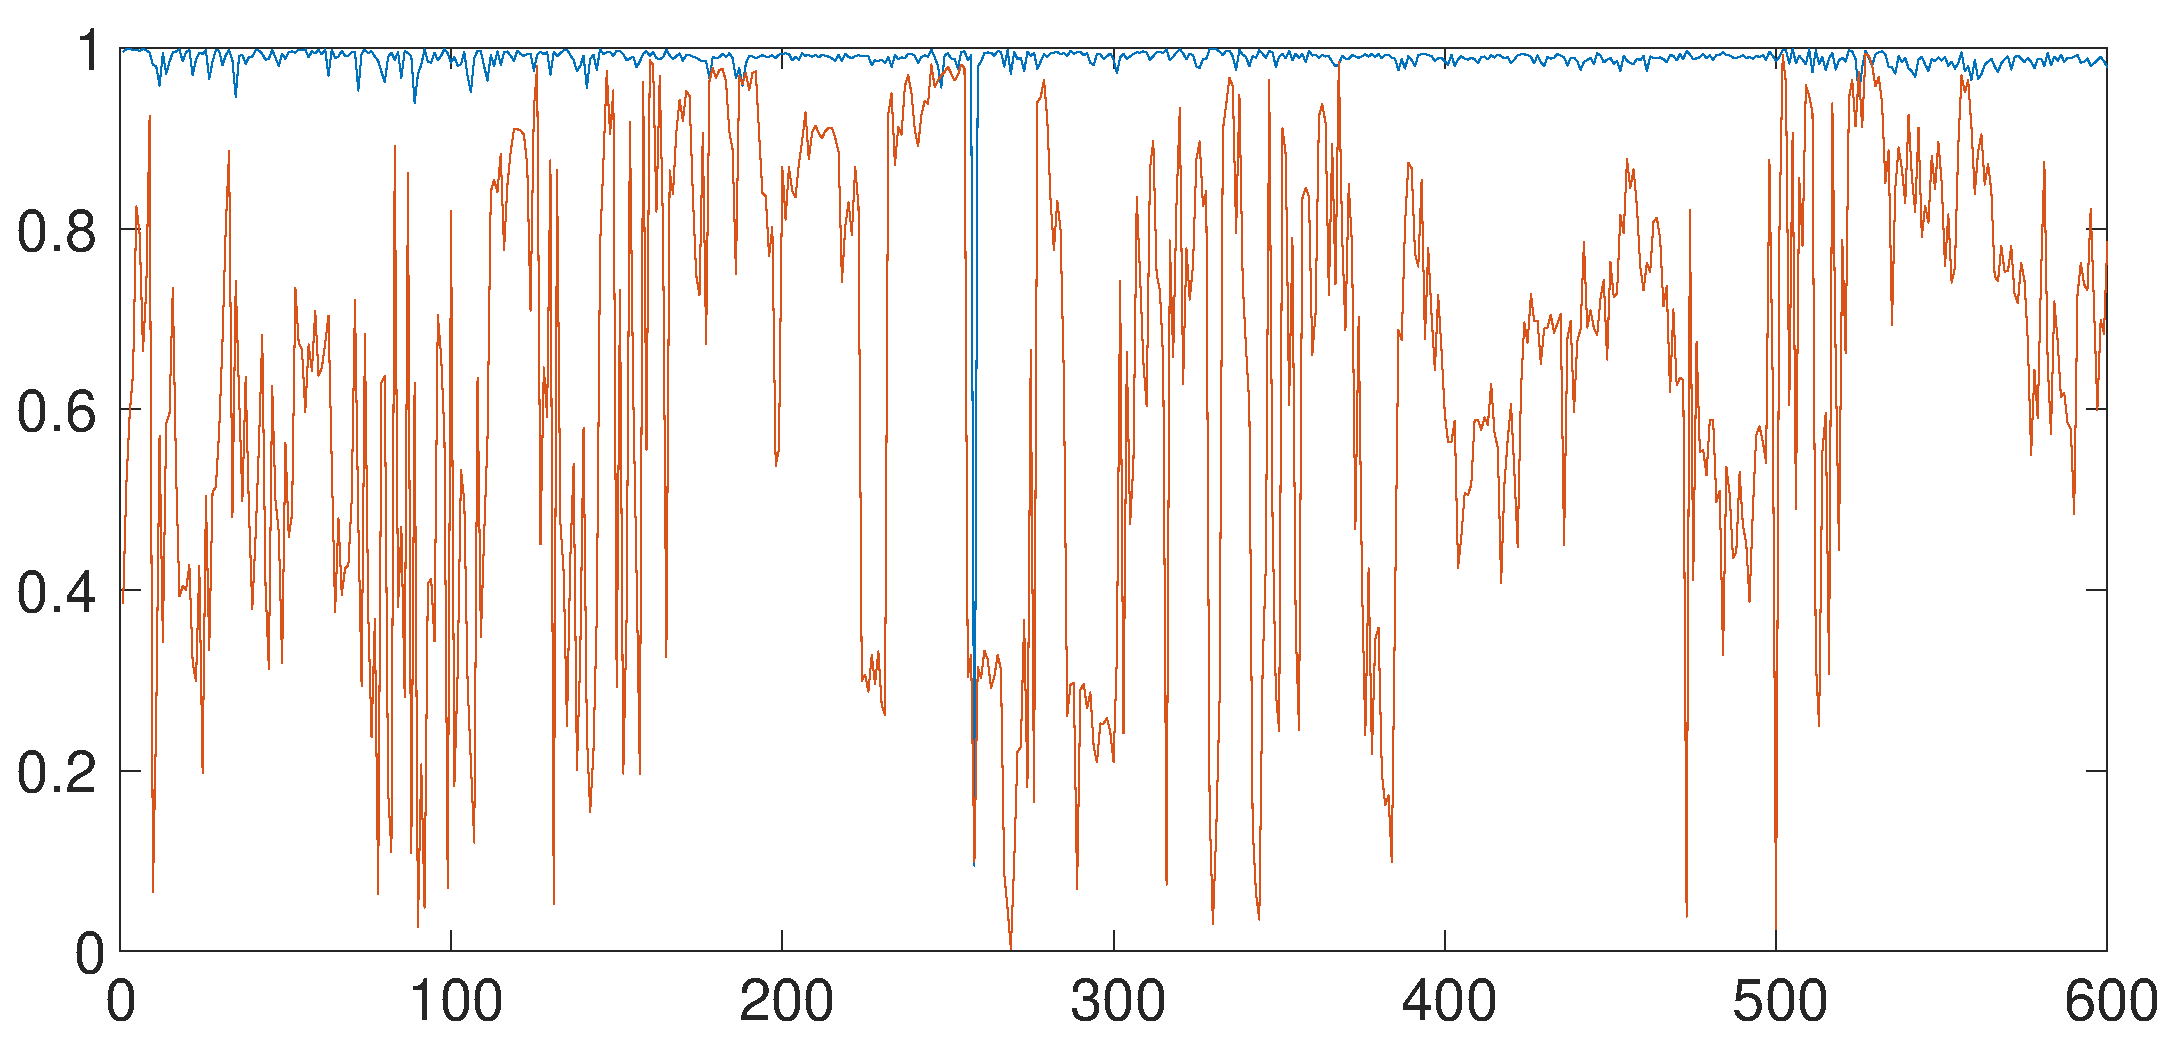
\includegraphics[width=0.3\textwidth]{images/tdd-xcorr/corridor-no-move.eps}
    }
    \subfigure[走廊-方式2]{
        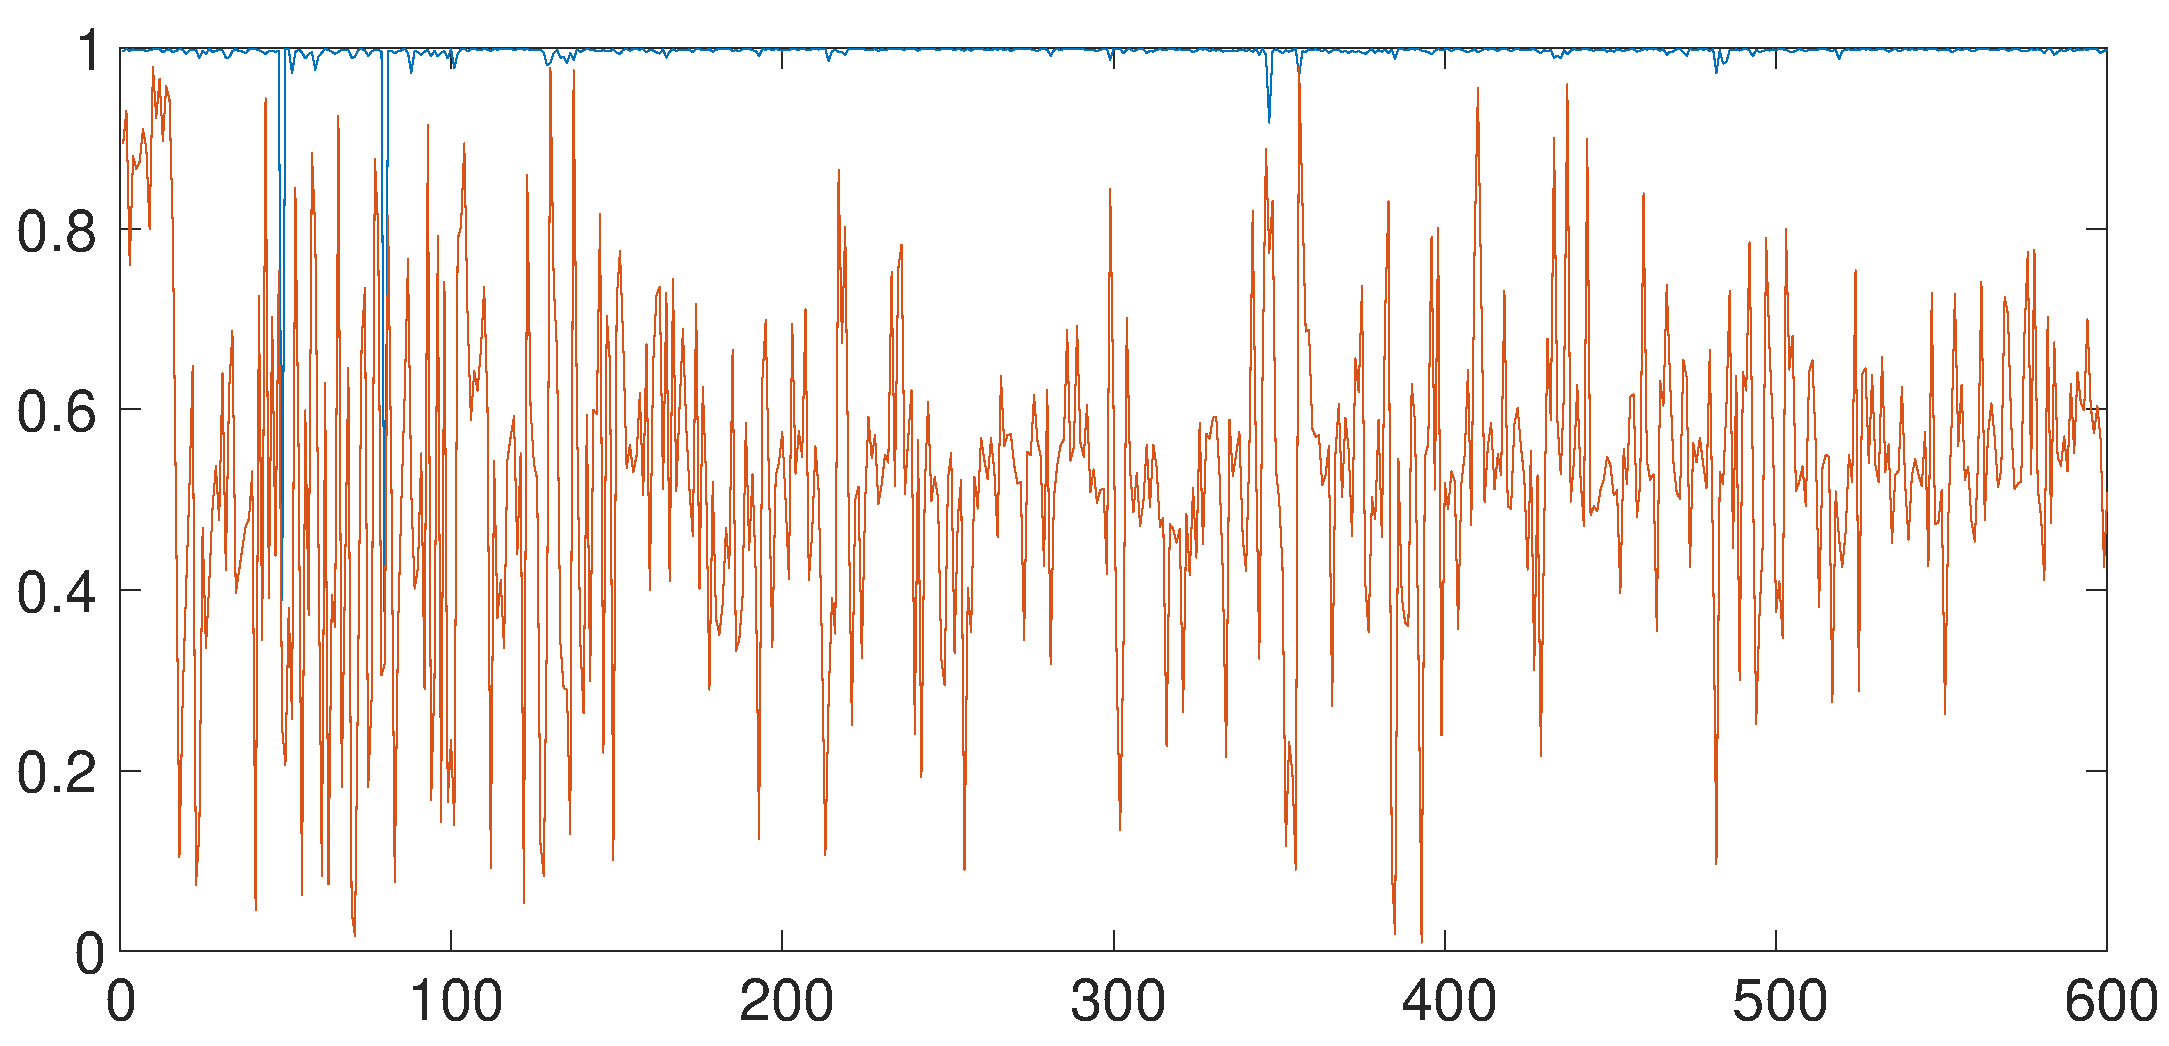
\includegraphics[width=0.3\textwidth]{images/tdd-xcorr/corridor-people-move.eps}
    }
    \subfigure[走廊-方式3]{
        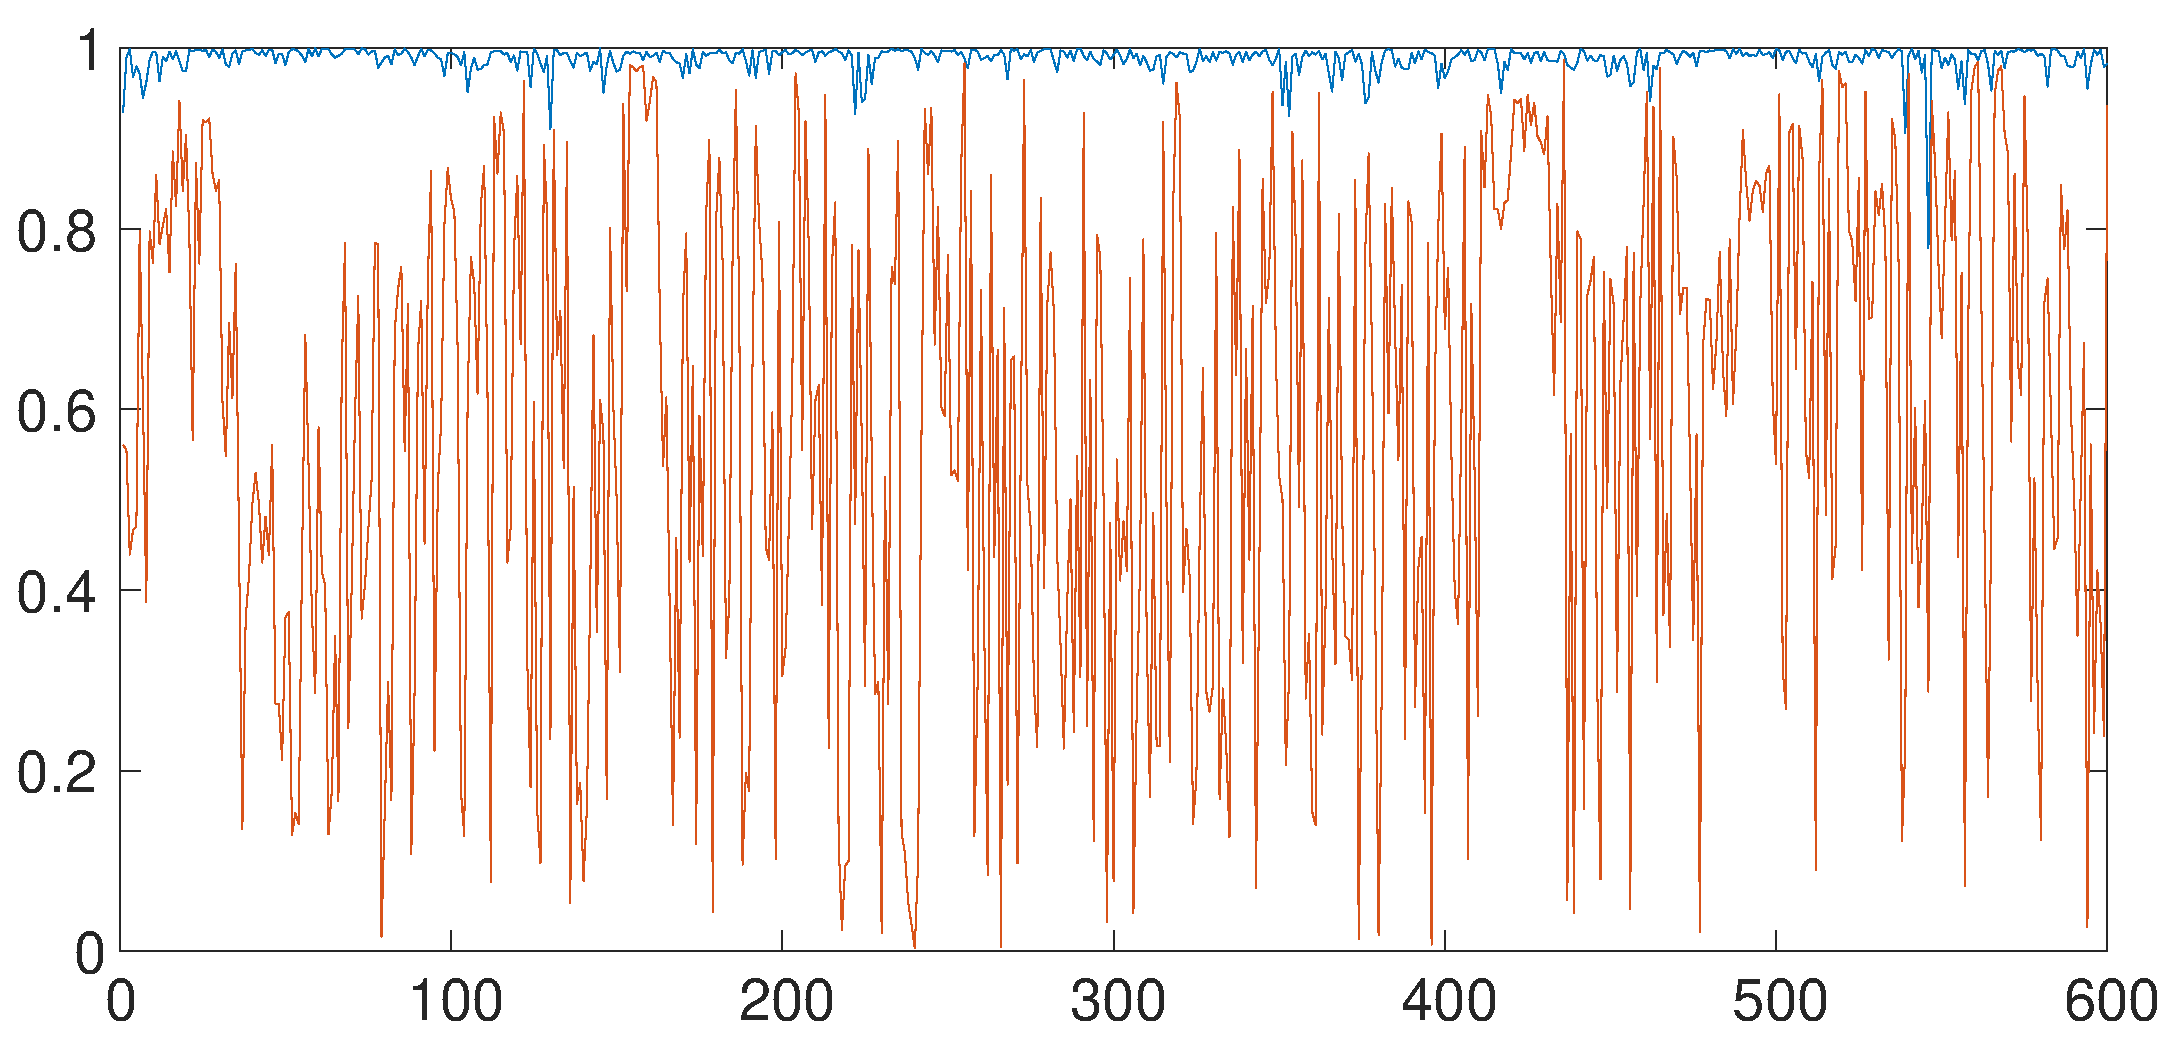
\includegraphics[width=0.3\textwidth]{images/tdd-xcorr/corridor-trolly-move.eps}
    }
    \quad
    \subfigure[室外-方式1]{
        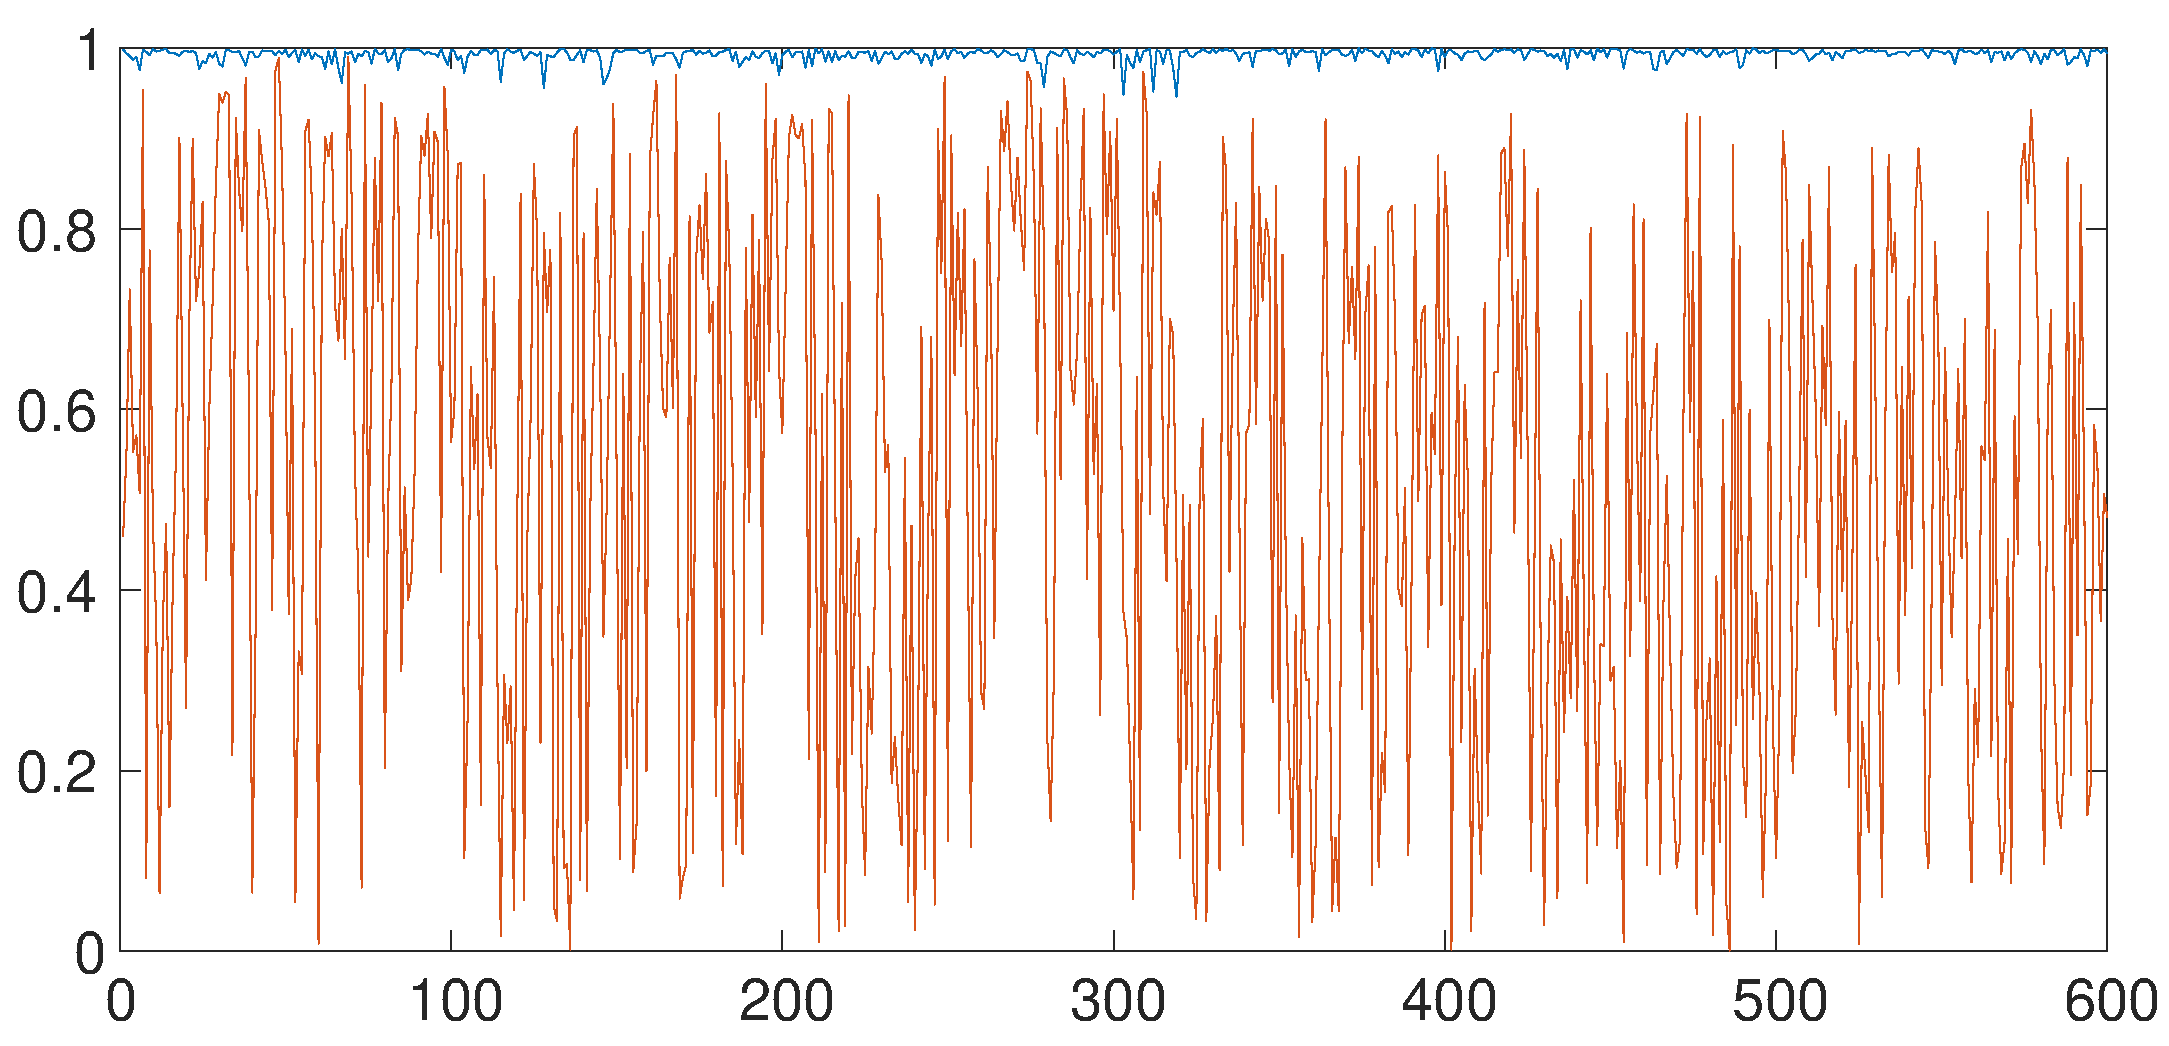
\includegraphics[width=0.3\textwidth]{images/tdd-xcorr/outdoor-no-move.eps}
    }
    \subfigure[室外-方式2]{
        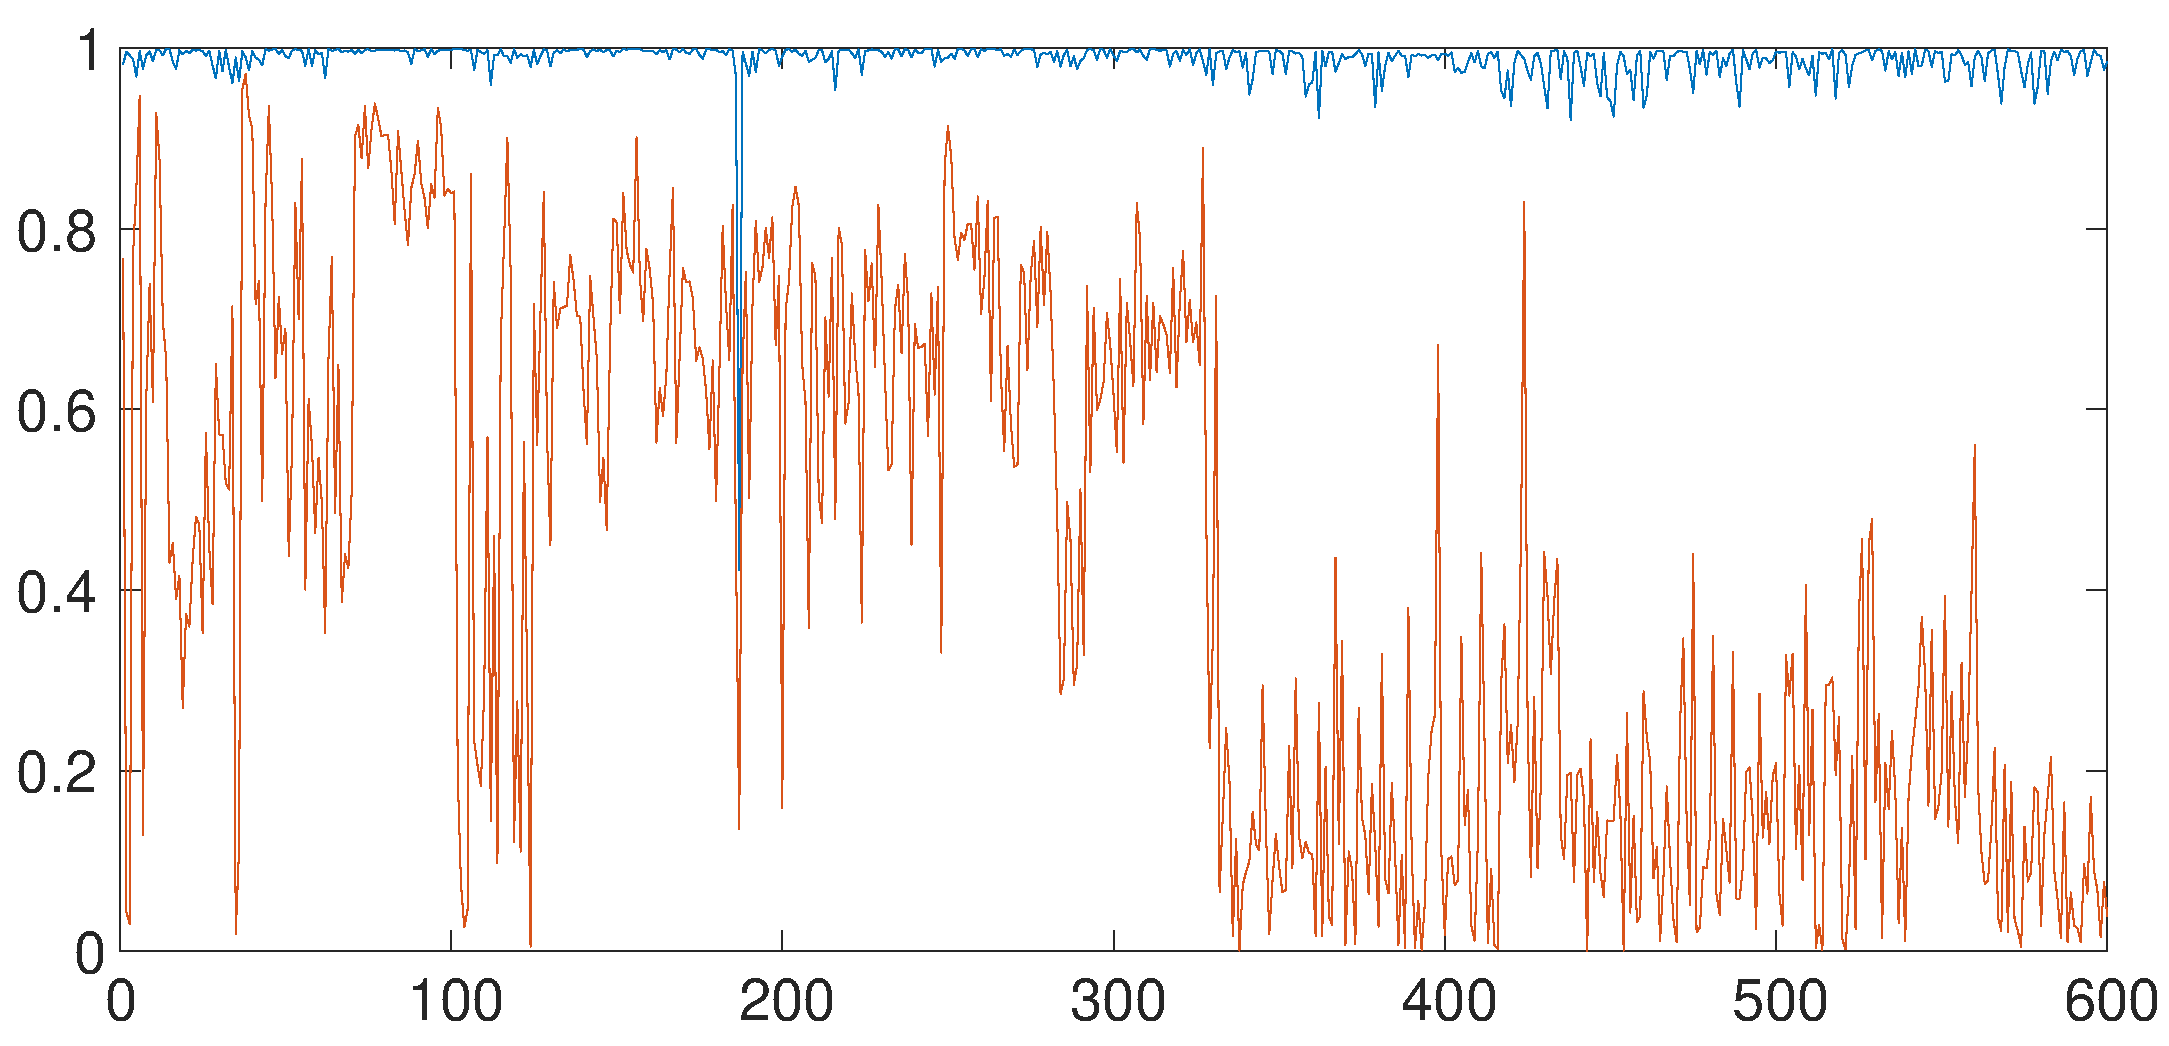
\includegraphics[width=0.3\textwidth]{images/tdd-xcorr/outdoor-people-move.eps}
    }
    \subfigure[室外-方式3]{
        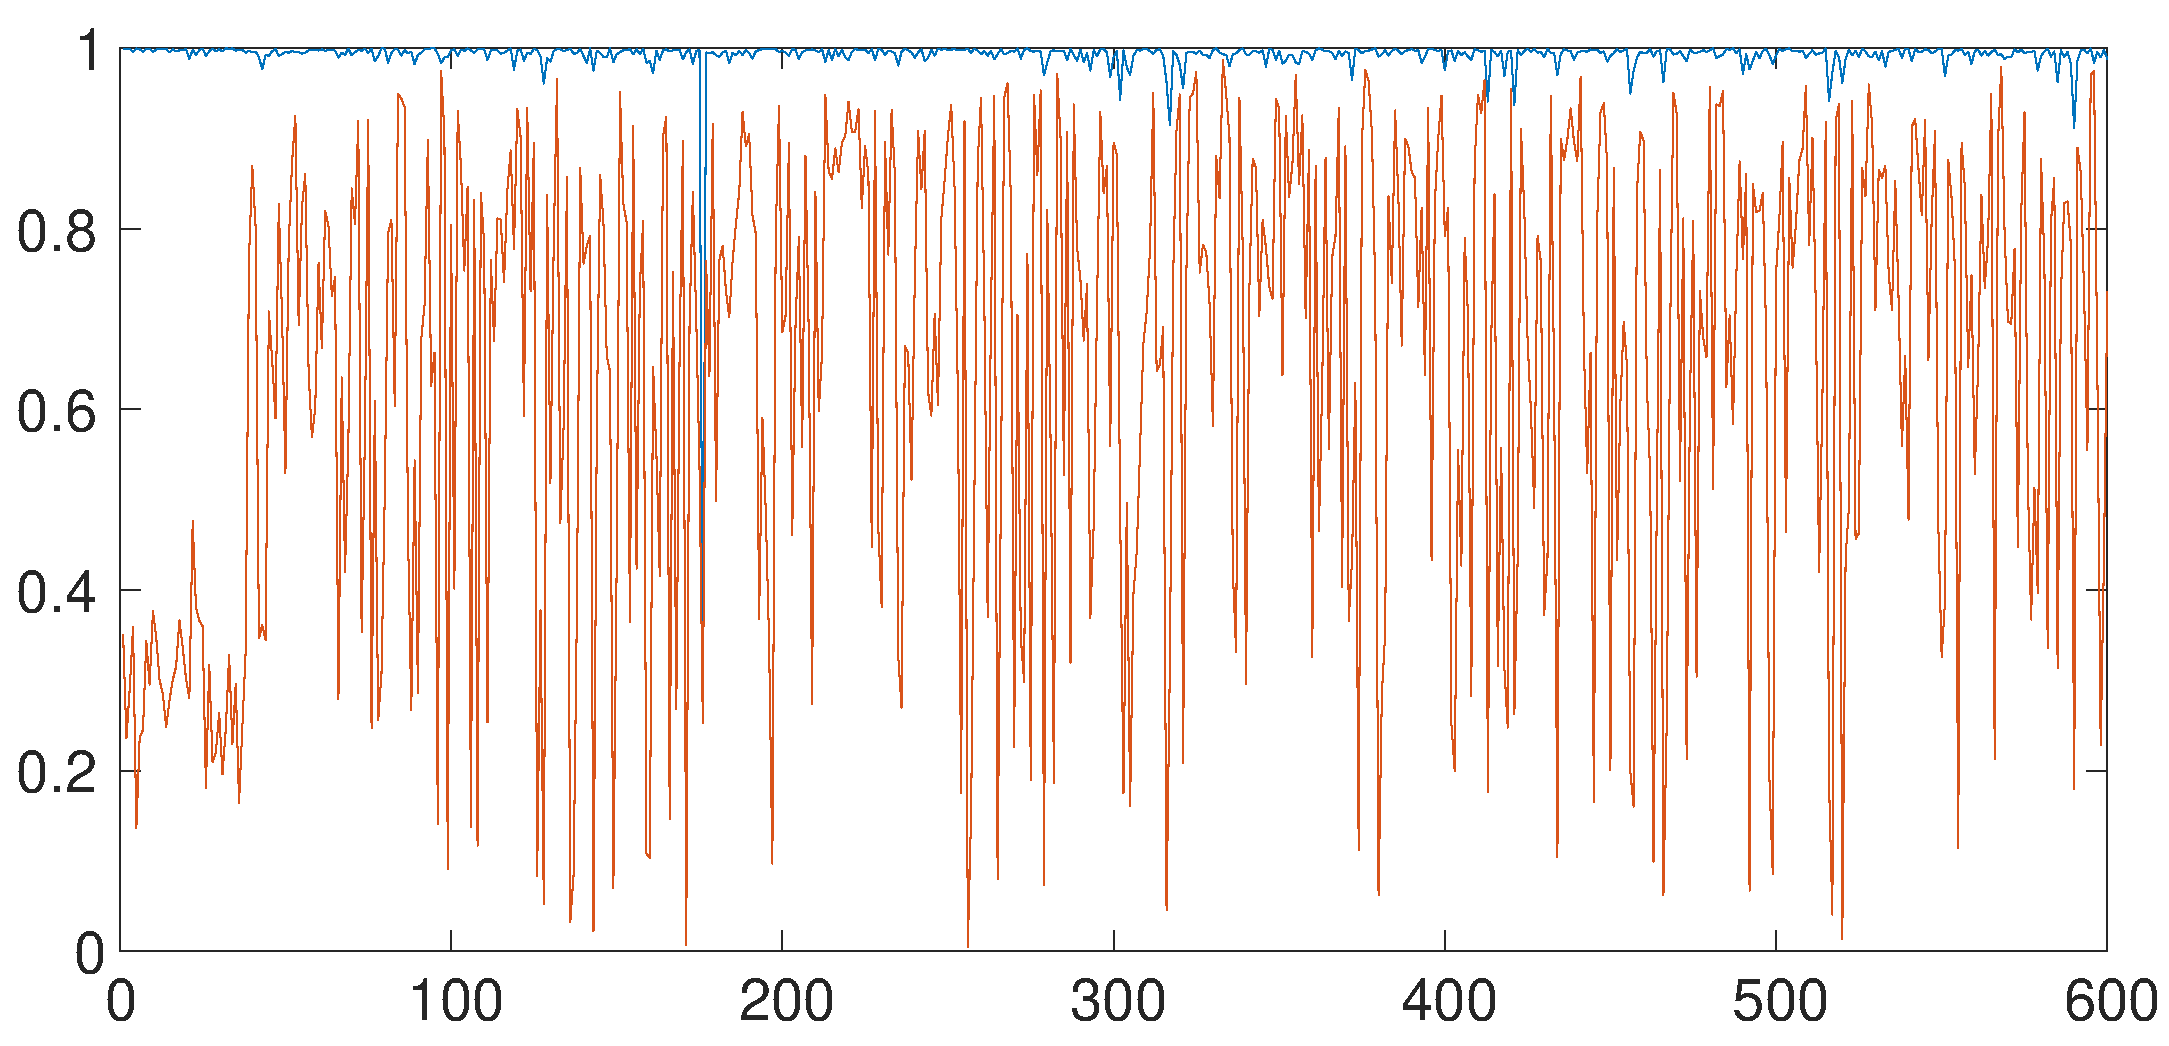
\includegraphics[width=0.3\textwidth]{images/tdd-xcorr/outdoor-trolly-move.eps}
    }
    \caption{不同场景与环境下Alice和Bob、Alice和Eve之间CSI相关系数}{} % xcorr between alice and bob, xcorr between bob and eve
    \label{tdd_csi_xcorr}
\end{figure}

将多组数据取平均,得到9种情况下,Alice、Bob和Eve之间的平均皮尔逊相关系数如图\ref{tdd_bar_xcorr}所示。分析结果表明,在9种情况下,Alice与Bob之间相关性均远高于Alice与Eve。无论哪种情况,Alice和Bob之间相关系数均高于0.9711,该情况出现在室内终端移动的情况下,Alice和Bob之间相关系数最高出现在室内房间终端固定的情况下,高达0.9963。而Alice与Eve之间相关系数最高也只有0.8192,并且出现在室内房间终端固定的情况下。无论是室内、走廊还是室外,当有人员在周围环境走动时,Alice与Eve之间的信道相关性最低,其中室内终端移动情况下低至0.4004。

\begin{figure}[htbp!]
    \centering 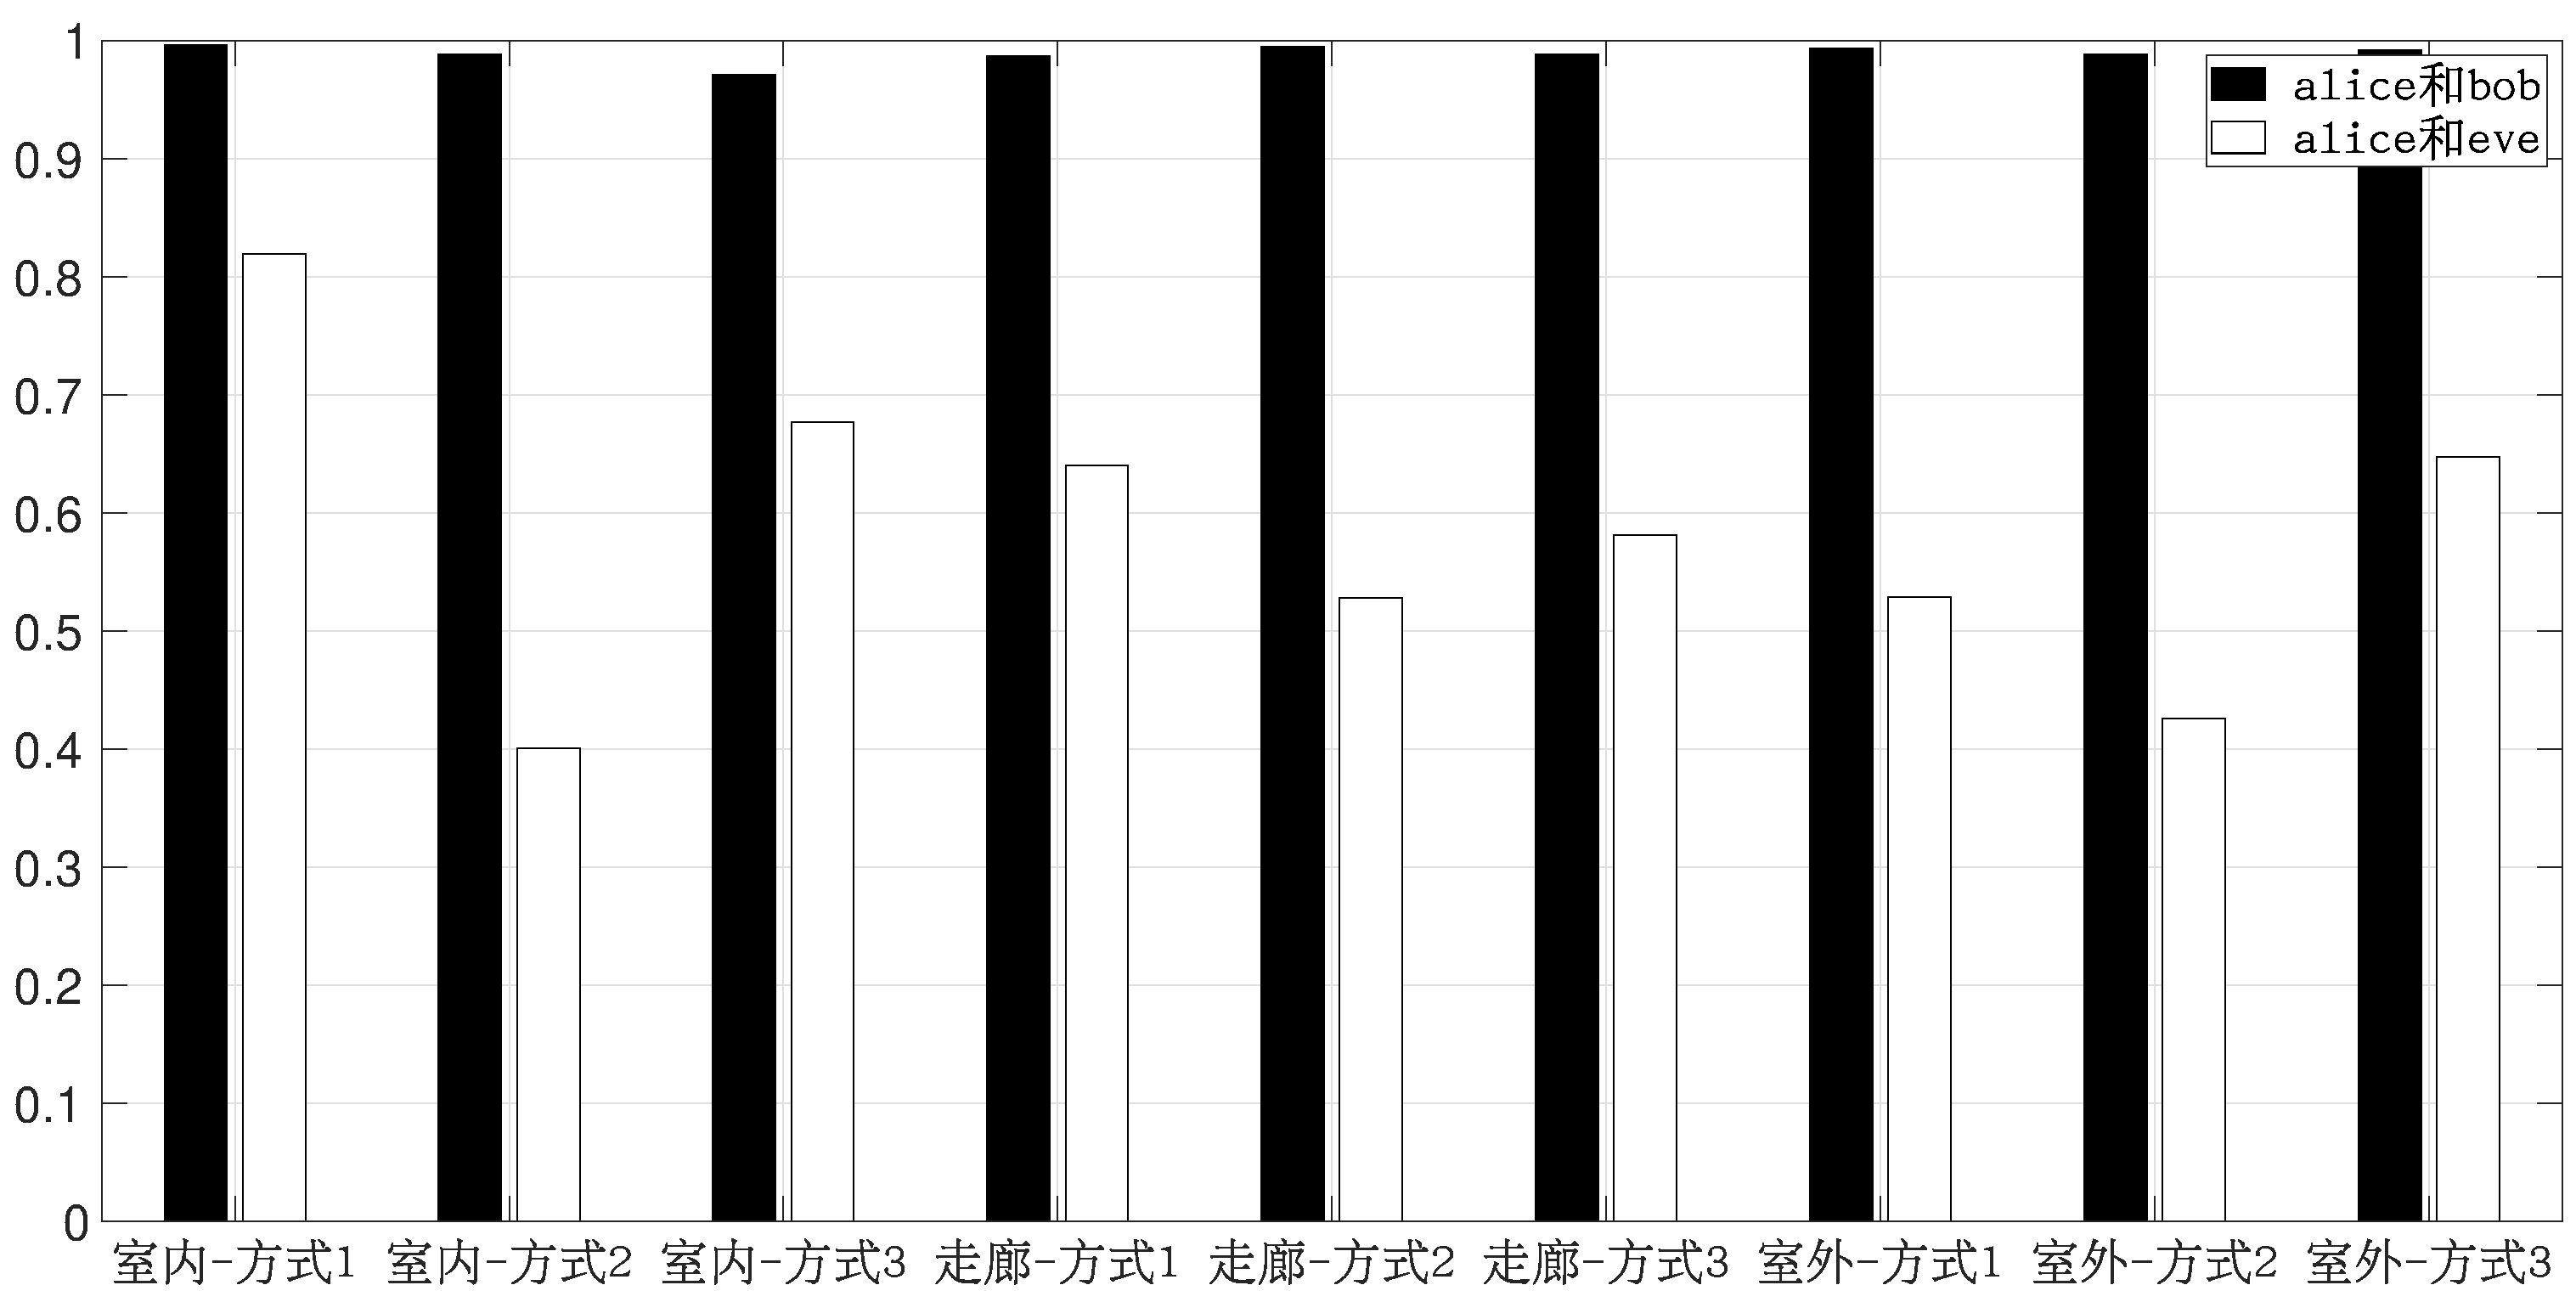
\includegraphics[width=0.9\textwidth]{images/tdd-xcorr/bar2.eps}
    \caption{不同场景下三者之间的互相关系数柱状图}
    \label{tdd_bar_xcorr}
\end{figure}

\subsection{信息泄漏率}

虽然第三方在无线密钥生成过程中通过相同生成步骤得到相同的会话密钥,但是对无线密钥生成的所有过程对于第三方来说都是完全透明的\cite{sahin2016secure},第三方可以在信道探测过程探测导频信号、在信息调和过程中窃听调和信息,因此本文通过信息论中未泄露的信息量来评估系统的安全性。

本文在9种情况下按照公式(\ref{safe_rate_equation})计算了多组安全信息率并取平均,9种情况下的平均安全信息率如图\ref{tdd_bar_leak}所示。从图中可知,无论是室内、走廊还是室外,均是当有人员在周围环境走动时安全信息率最高,其中在室外,信息安全比率高达91.01\%,这也是所有情况中的最高值,在走廊,信息安全比率为78.52\%。在所有情况中,室内房间终端移动时的信息安全比率最低,低至67.05\%。9种情况的平均安全信息率具体数据为表\ref{tdd_bar_leak_data}。


\begin{figure}[htbp!]
    \centering 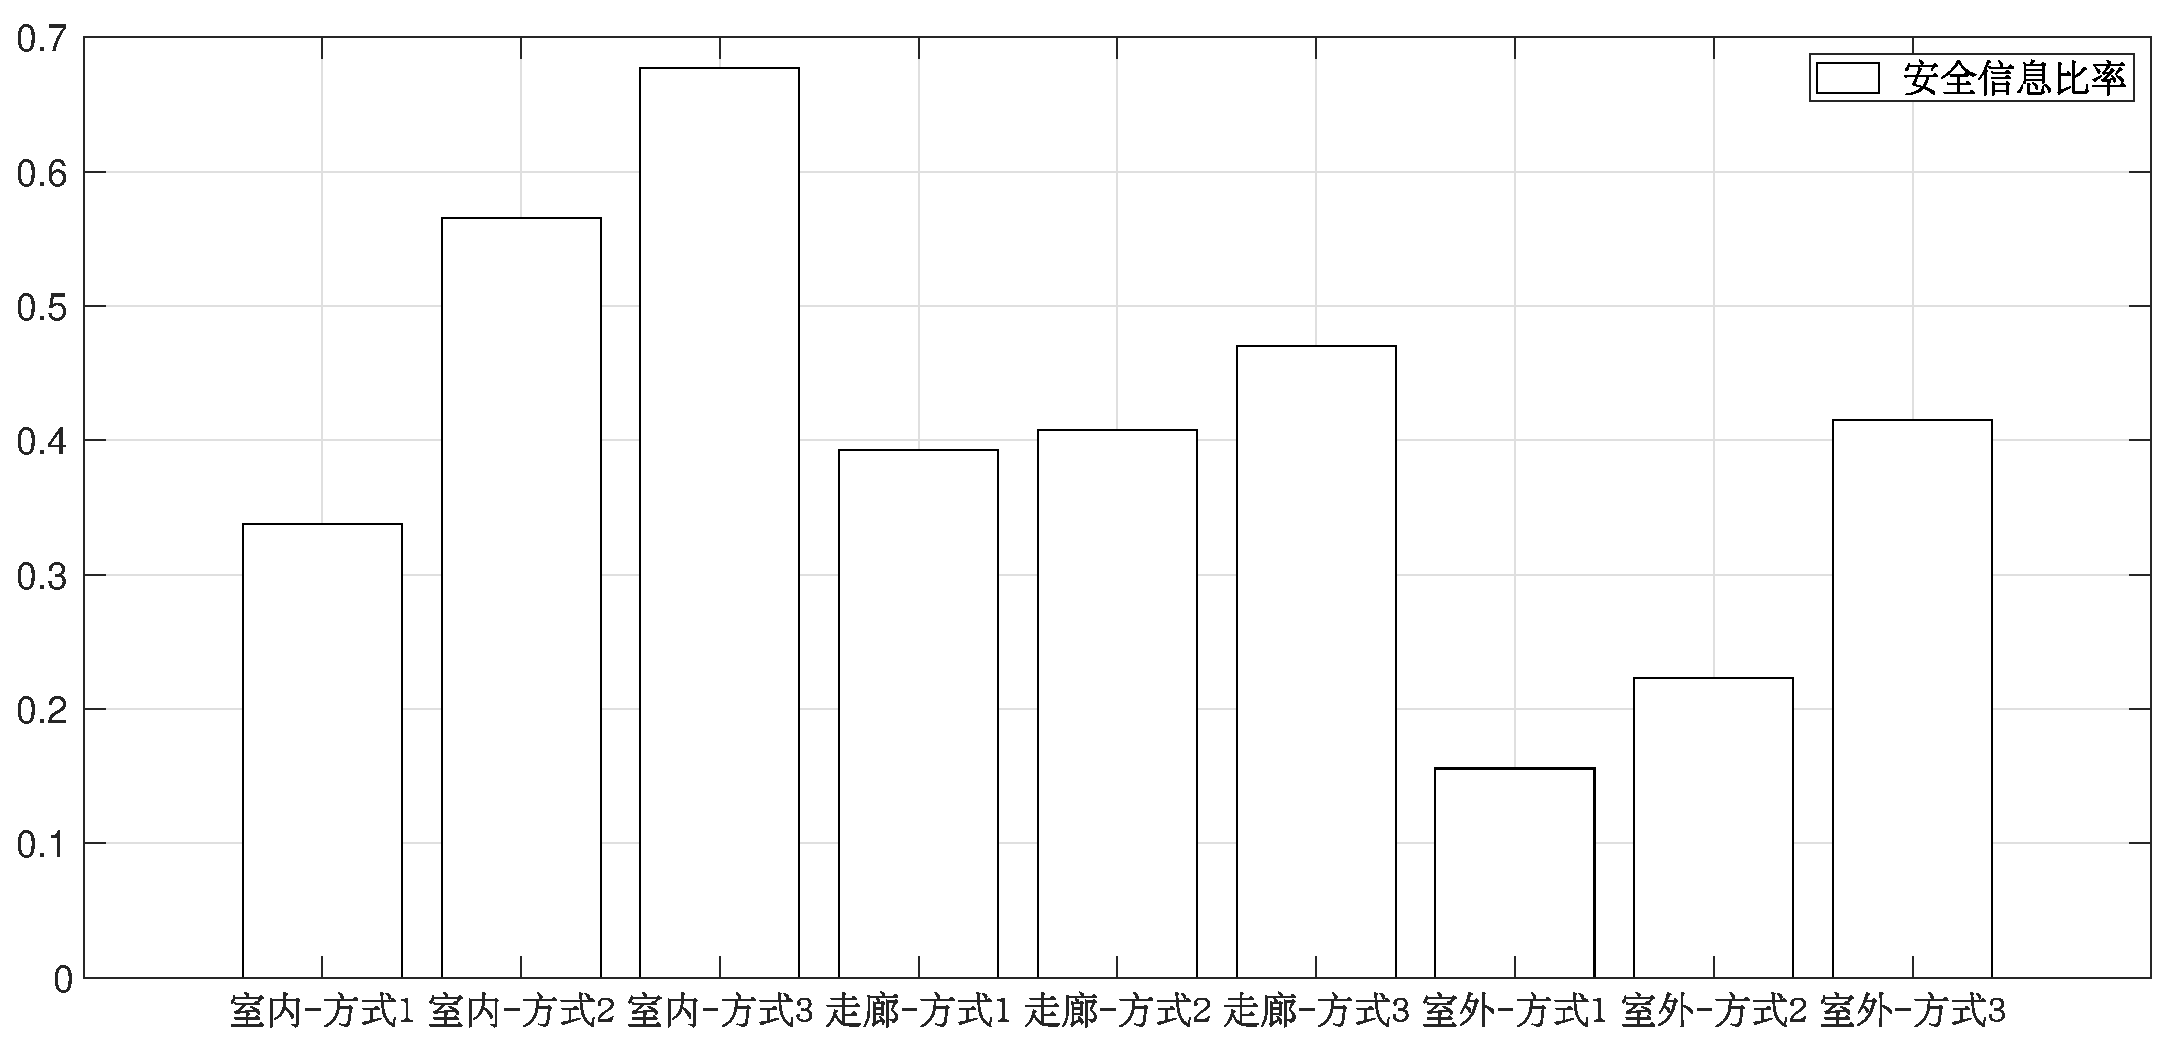
\includegraphics[width=0.9\textwidth]{images/tdd-leak/bar.eps}
    \caption{不同场景下的平均安全信息率柱状图}
    \label{tdd_bar_leak}
\end{figure}

% \begin{table}[!ht]
%     \centering
%     \begin{tabular*}{\hsize}{@{}@{\extracolsep{\fill}}|c|c|c|c|@{}}
%     \toprule
%         & \textbf{方式1} & \textbf{方式2} & \textbf{方式3} \\
%     \midrule
%     室内 & 0.7962 & 0.8924 & 0.6705 \\ 
% 	走廊 & 0.7604 & 0.7852 & 0.7725 \\ 
%     室外 & 0.8177 & 0.9101 & 0.7882 \\
%     \bottomrule
%     \end{tabular*}
%     \caption{不同场景下的平均安全信息率数值
%     \label{tdd_bar_leak_data}}
% \end{table}

\begin{table}[htbp] % 依赖包 booktabs
    \centering
    \setlength{\tabcolsep}{16mm}{
    \begin{tabular}{cccc}
    \toprule
        & \textbf{方式1} & \textbf{方式2} & \textbf{方式3} \\
    \midrule
    室内 & 0.7962 & 0.8924 & 0.6705 \\ 
	走廊 & 0.7604 & 0.7852 & 0.7725 \\ 
    室外 & 0.8177 & 0.9101 & 0.7882 \\
    \bottomrule
    \end{tabular}
    }
    \caption{不同场景下的平均安全信息率数值
    \label{tdd_bar_leak_data}}
\end{table}


本文计算出室内、走廊、室外三种场景下,所有信道环境下的安全信息率平均值,如表\ref{three_scene_avg}所示。表中结果说明各种信道环境下,室外的信息安全比率最高,高达83.87\%,走廊的信息安全比率最低,低至77.27\%。也计算出终端固定、人员移动、终端移动三种信道环境下,所有场景的安全信息率平均值,如表\ref{three_channel_env_avg}。表中说,各种场景下,人员移动的安全比率最高,高达86.26\%,终端移动的安全比率最低,低至74.37\%。从结果中可以看出,信道适当的变化可以提高无线密钥生成系统的信息安全比率。室内和走廊的平均值相近,说明室内和走廊场景对安全信息比率影响相似,室外场景会提高安全信息比率。相对于终端固定和终端移动的信道环境,人员移动对信息安全比率有很大的改善。


\begin{table}[]
    \centering
    \setlength{\tabcolsep}{22mm}{
    \begin{tabular}{ccc}
    \toprule
    室内 & 走廊 & 室外 \\ 
    \midrule
    78.64\% & 77.27\% & 83.87\% \\ 
    \bottomrule
    \end{tabular}
    }
    \caption{室内、走廊和室外三种场景的平均安全信息率
    \label{three_scene_avg}}
\end{table}

\begin{table}[]
    \centering
    \setlength{\tabcolsep}{20mm}{
    \begin{tabular}{ccc}
    \toprule
    终端固定 & 人员移动 & 终端移动 \\
    \midrule
    79.14\% & 86.26\% & 74.37\% \\ 
    \bottomrule
    \end{tabular}
    }
    \caption{终端固定、人员走动和终端移动三种信道环境的平均安全信息率
    \label{three_channel_env_avg}}
\end{table}

\subsection{随机性评估}

本文使用两种指标来作系统的随机性评估,使用频域的图像熵以及NIST随机性测试分别评估CSI随机性和密钥随机性。

\subsubsection{CSI随机性}

本文在理论基础部分提出了用图像熵评估CSI随机性的理论依据,CSI的图像熵展示了时域以及频域的变化。为了更好的对比,本文计算了信道无多径且不随时间变化、信道有多径且不随时间变化、信道随时间不同完全随机变化三种特殊情况下的CSI作为对比,其CSI如图\ref{special_csi}所示,三种特殊情况对应熵值如表\ref{entropy_spectial}所示。信道完全无多径且不变化时,图像熵接近于0,信道有多径且不随时间变化时稍大,但也接近于0。当信道随时间不同完全随机的情况下,图像熵为7.0098。因此本文测量数据计算出的CSI图像熵应该出现在0.00006~7.0098之间。

\begin{figure}
    \centering
    \subfigure[信道无多径且不随时间变化]{
      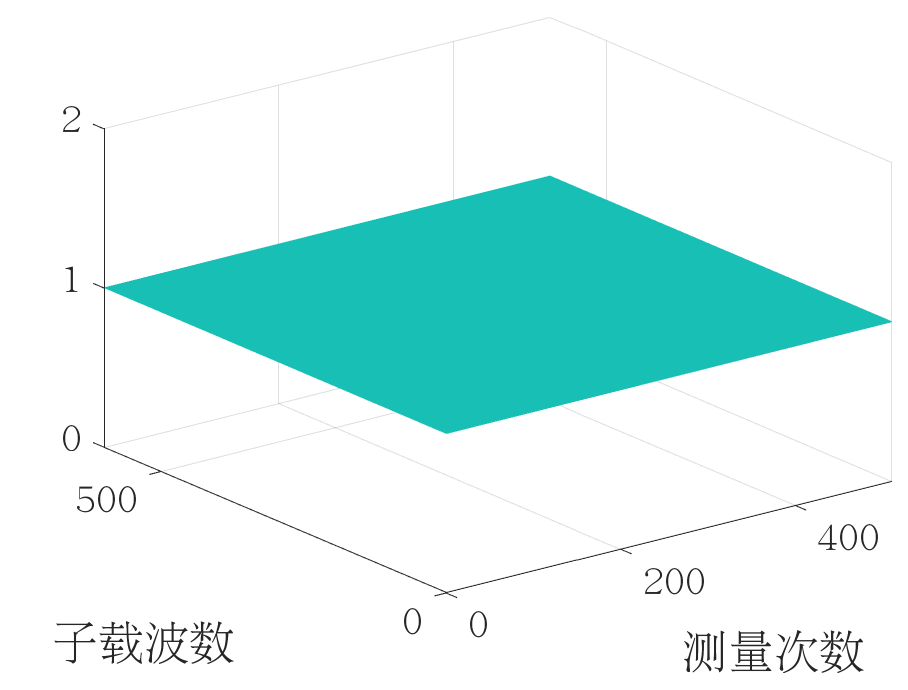
\includegraphics[width=0.3\textwidth]{images/spectial-entropy/constant.eps}
    }
    \subfigure[信道有多径且不随时间变化]{
      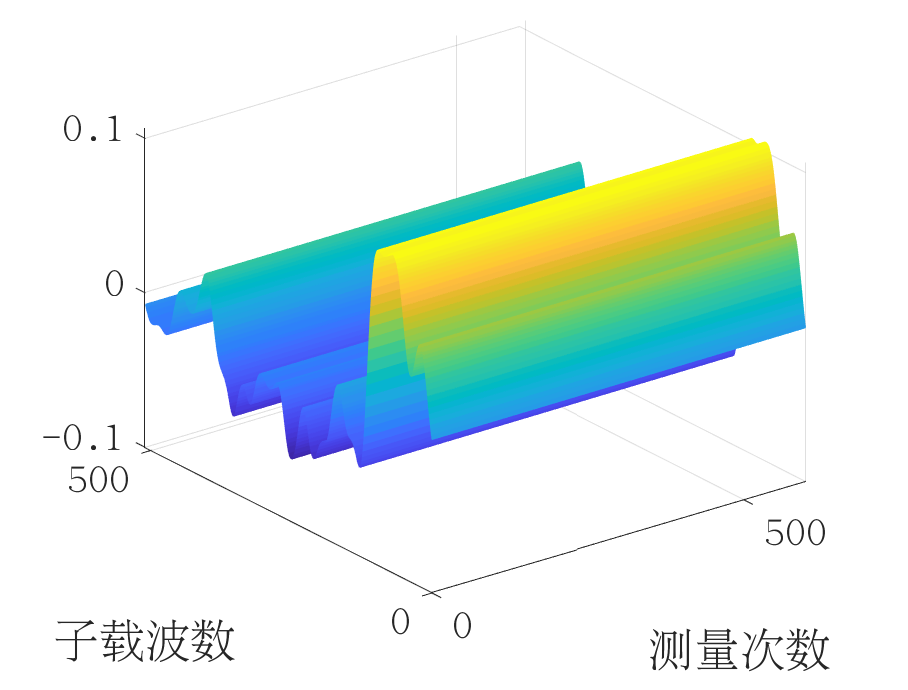
\includegraphics[width=0.3\textwidth]{images/spectial-entropy/multipath.eps}
    }
    \subfigure[信道随时间不同完全随机变化]{
      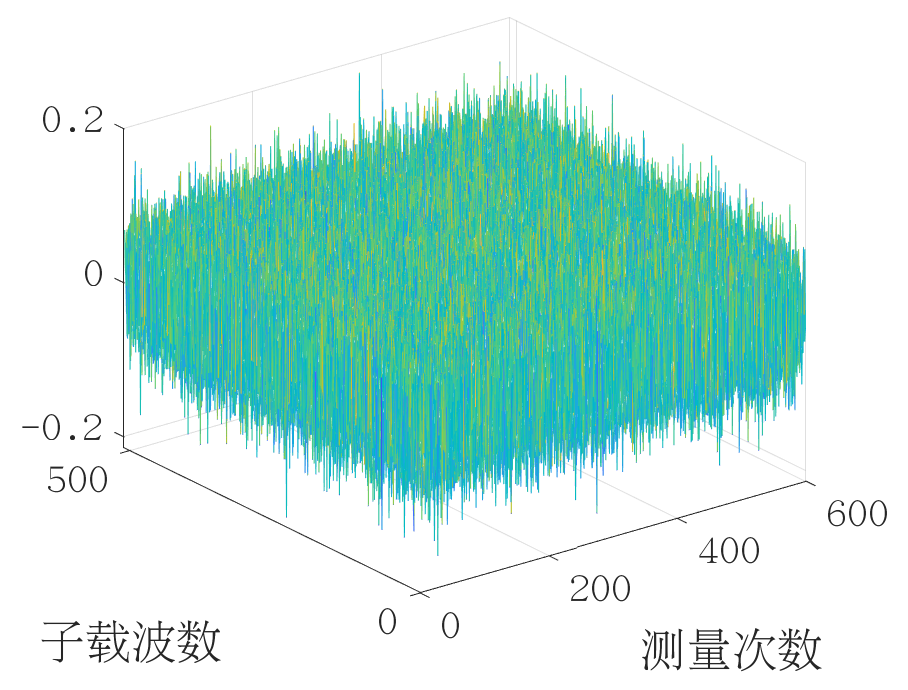
\includegraphics[width=0.3\textwidth]{images/spectial-entropy/random.eps}
    }
    \caption{特殊情况下CSI结果展示}{} % xcorr between alice and bob, xcorr between bob and eve
    \label{special_csi}
\end{figure}

\begin{table}[]
    \centering
    \setlength{\tabcolsep}{4mm}{
    \begin{tabular}{ccc}
        \toprule
        \textbf{信道无多径且不随时间变化} & \textbf{信道有多径且不随时间变化} & \textbf{信道随时间不同完全随机变化} \\
        \midrule
        0.00006 & 0.0262 & 7.0098 \\
        \bottomrule
    \end{tabular}
    }
    \caption{特殊情况的图像熵值
    \label{entropy_spectial}}
\end{table}

\begin{table}[]
    \centering
    \setlength{\tabcolsep}{16mm}{
    \begin{tabular}{cccc} 
        \toprule
        & \textbf{方式1} & \textbf{方式2} & \textbf{方式3} \\
        \midrule
        室内 & 2.5391 & 3.7227 & 3.9960 \\ 
        走廊 & 3.3293 & 3.8674 & 4.0667 \\ 
        室外 & 3.8696 & 3.8933 & 4.0924 \\
        \bottomrule
    \end{tabular}
    }
    \caption{不同场景的图像熵值
    \label{entropy_fft2d}}
\end{table}

本文在每个情况下,使用600组CSI按照公式(\ref{entropy_fft2d_equation})计算多组CSI的图像熵,如表\ref{entropy_fft2d}。从表中可以看出,无论哪种信道环境,室内房间的CSI随机性均最低,空旷室外的CSI随机性最高。无论哪种场景,终端固定的信道环境下的CSI随机性最低,终端移动的信道环境下的CSI随机性最高。所有情况中,在室内场景下的终端固定时CSI随机性最低,低至2.5391;在室外场景下的终端移动时CSI随机性最高,高达4.0924。从表中分析得知,随着信道环境更加复杂,系统探测的CSI随机性也会增加。

\subsubsection{密钥随机性}

本文选择NIST随机性测试中的7种随机性测试方法计算不同场景下生成密钥的随机性。本文分别计算了降采样率为1、4、8时的测试结果,分别如表\ref{NIST_test_result_1}、\ref{NIST_test_result_4}、\ref{NIST_test_result_8}所示。图中数据为,600组数据中,通过NIST测试的比例,在图中标记出比例小于1\%的数据。从图中可以看出,随着降采样率提高,比率小于1\%的数据减少,密钥随机性提高。在降采样率为1时,多组数据在NIST随机性测试中表现很差,在降采样率为8时,系统生成的密钥数据在NIST随机性测试中表现良好。表中结果也表明,室内房间场景下终端固定的信道环境中,密钥随机性最低,在多项NIST随机性测试中,通过NIST测试的比率最低。

% 参考 https://blog.csdn.net/ch1209498273/article/details/78848464


\begin{table}[]
    \centering
    \tabulinesep=1.2mm
    \begin{tabu}to \linewidth{X[c,m]X[c,m]X[c,m]X[c,m]X[c,m]X[c,m]X[c,m]X[c,m]X[c,m]X[c,m]}
        \toprule
        \textbf{} & \textbf{室内-方式1} & \textbf{室内-方式2} & \textbf{室内-方式3} & \textbf{走廊-方式1} & \textbf{走廊-方式2} & \textbf{走廊-方式3} & 
        \textbf{室外-方式1} & \textbf{室外-方式2} & \textbf{室外-方式3} \\
        \midrule
        频率检验 & 11.53\%    & 12.65\%    & 05.94\%    & 03.67\%    & 01.20\%    & 06.83\%    & 02.74\%    & 12.52\%    & 04.10\% \\
        块内频数检验 & \underline{00.00\%}    & 07.02\%    & 15.75\%    & \underline{00.09\%}    & 01.09\%    & 02.57\%    & \underline{00.44\%}    & \underline{00.81\%}    & 01.49\% \\
        游程检验 & 57.01\%    & \underline{00.81\%}    & \underline{00.48\%}    & 07.21\%    & \underline{00.33\%}    & 02.57\%    & 01.06\%    & 01.67\%    & 01.30\% \\
        块内最长游程检验 & \underline{00.00\%}    & \underline{00.00\%}    & \underline{00.06\%}    & \underline{00.00\%}    & \underline{00.00\%}    & \underline{00.00\%}    & \underline{00.00\%}    & \underline{00.06\%}    & \underline{00.06\%} \\
        % 二元矩阵秩检验 & 0.9953    & 0.9787    & 0.9352    & 0.9949    & 0.9978    & 0.9812    & 0.9994    & 0.9734    & 0.9689 \\
        序列检验 & 20.56\%    & \underline{00.29\%}    & \underline{00.42\%}    & 02.14\%    & \underline{00.11\%}    & 01.63\%    & \underline{00.44\%}    & 01.12\%    & \underline{00.87\%} \\
        近似熵检验 & 21.65\%    & \underline{00.23\%}    & \underline{00.55\%}    & 02.19\%    & \underline{00.11\%}    & 01.57\%    & \underline{00.50\%}    & 01.12\%    & \underline{00.87\%} \\
        累加和检验 & 78.04\%    & 77.34\%    & 65.78\%    & 63.46\%    & 66.63\%    & 73.23\%    & 75.73\%    & 82.40\%    & 76.46\% \\
        \bottomrule
    \end{tabu}
    \caption{NIST测试结果 降采样数为1
    \label{NIST_test_result_1}}
\end{table}

\begin{table}[]
    \centering
    \tabulinesep=1.2mm        
    \begin{tabu}to \linewidth{X[c,m]X[c,m]X[c,m]X[c,m]X[c,m]X[c,m]X[c,m]X[c,m]X[c,m]X[c,m]}
        \toprule
        \textbf{} & \textbf{室内-方式1} & \textbf{室内-方式2} & \textbf{室内-方式3} & \textbf{走廊-方式1} & \textbf{走廊-方式2} & \textbf{走廊-方式3} & 
        \textbf{室外-方式1} & \textbf{室外-方式2} & \textbf{室外-方式3} \\
        \midrule
        频率检验 & 09.33\%    & 36.17\%    & 21.33\%    & 14.33\%    & 39.67\%    & 23.67\%    & 22.83\%    & 15.17\%    & 20.33\% \\
        块内频数检验 & 42.33\%    & 67.83\%    & 85.67\%    & 88.00\%    & 19.67\%    & 77.67\%    & 77.50\%    & 59.67\%    & 73.83\% \\
        游程检验 & \underline{00.83\%}    & 18.83\%    & 07.83\%    & 04.67\%    & 64.33\%    & 13.83\%    & 11.67\%    & 15.83\%    & 14.83\% \\
        块内最长游程检验 & \underline{00.67\%}    & \underline{00.83\%}    & 02.33\%    & 01.83\%    & 02.33\%    & 08.17\%    & \underline{00.67\%}    & 11.83\%    & 05.83\% \\
        % 二元矩阵秩检验 & 0.9750    & 0.9533    & 0.8683    & 0.9283    & 0.9783    & 0.8767    & 0.9950    & 0.8983    & 0.9200 \\
        序列检验 & \underline{00.00\%}    & 08.67\%    & 04.50\%    & 03.67\%    & 31.50\%    & 08.00\%    & 03.67\%    & 07.33\%    & 07.17\% \\
        近似熵检验 & \underline{00.00\%}    & 07.33\%    & 05.00\%    & 03.50\%    & 38.67\%    & 08.33\%    & 03.67\%    & 07.00\%    & 05.83\% \\
        累加和检验 & 90.50\%    & 89.50\%    & 86.17\%    & 80.17\%    & 80.17\%    & 90.83\%    & 88.17\%    & 95.33\%    & 90.00\% \\
        \bottomrule
    \end{tabu}
    \caption{NIST测试结果 降采样数为4
    \label{NIST_test_result_4}}
\end{table}


\begin{table}[]
    \centering
    % \setlength{\tabcolsep}{0.2mm}{
    \tabulinesep=1.2mm        
    \begin{tabu} to \linewidth{X[c,m]X[c,m]X[c,m]X[c,m]X[c,m]X[c,m]X[c,m]X[c,m]X[c,m]X[c,m]}
        \toprule
        \textbf{} & \textbf{室内-方式1} & \textbf{室内-方式2} & \textbf{室内-方式3} & \textbf{走廊-方式1} & \textbf{走廊-方式2} & \textbf{走廊-方式3} & 
        \textbf{室外-方式1} & \textbf{室外-方式2} & \textbf{室外-方式3} \\
        \midrule
        频率检验 & 32.00\%    & 63.33\%    & 54.50\%    & 55.67\%    & 65.50\%    & 49.00\%    & 58.00\%    & 30.50\%    & 41.50\%  \\
        块内频数检验 & 99.50\%    & 99.67\%    & 98.67\%    & 99.17\%    & 99.50\%    & 99.17\%    & 00.00\%    & 99.33\%    & 99.67\% \\
        游程检验 & 17.83\%    & 39.33\%    & 18.50\%    & 16.17\%    & 80.17\%    & 42.00\%    & 29.50\%    & 46.83\%    & 38.17\% \\
        块内最长游程检验 & 70.17\%    & 42.50\%    & 25.00\%    & 26.50\%    & 91.00\%    & 48.83\%    & 42.17\%    & 76.67\%    & 54.83\% \\
        % 二元矩阵秩检验 & 0.0000    & 0.0000    & 0.0000    & 0.0000    & 0.0000    & 0.0000    & 0.0000    & 0.0000    & 0.0000 \\
        序列检验 & 03.17\%    & 30.00\%    & 12.50\%    & 11.17\%    & 63.00\%    & 26.67\%    & 19.67\%    & 22.50\%    & 23.50\% \\
        近似熵检验 & 01.17\%    & 30.50\%    & 11.33\%    & 09.50\%    & 64.50\%    & 23.17\%    & 17.33\%    & 20.67\%    & 21.33\% \\
        累加和检验 & 100.00\%    & 98.00\%    & 98.50\%    & 98.67\%    & 99.17\%    & 98.83\%    & 99.50\%    & 99.50\%    & 99.50\% \\
       
        \bottomrule
    \end{tabu}
    % }
    \caption{NIST测试结果 降采样数为8
    \label{NIST_test_result_8}}
\end{table}

\subsection{密钥生成速率}

调整降采样率可以影响密钥生成速率,降采样率过高,密钥生成速率降低,降采样率过低,密钥生成速率
提高,但密钥一致率会降低。本文计算了室内终端固定情况下,不同降采样率的密钥生成速率,如图\ref{keyrate}所示。观察可知,密钥生成速率随着降采样率升高而降低。在采样率
为 4 时,密钥生成速率高达 92.2231bits/s,在采样率为 20 时,密钥生成速率降低到 15.9688 bits/s。


\begin{figure}[htbp!]
    \centering 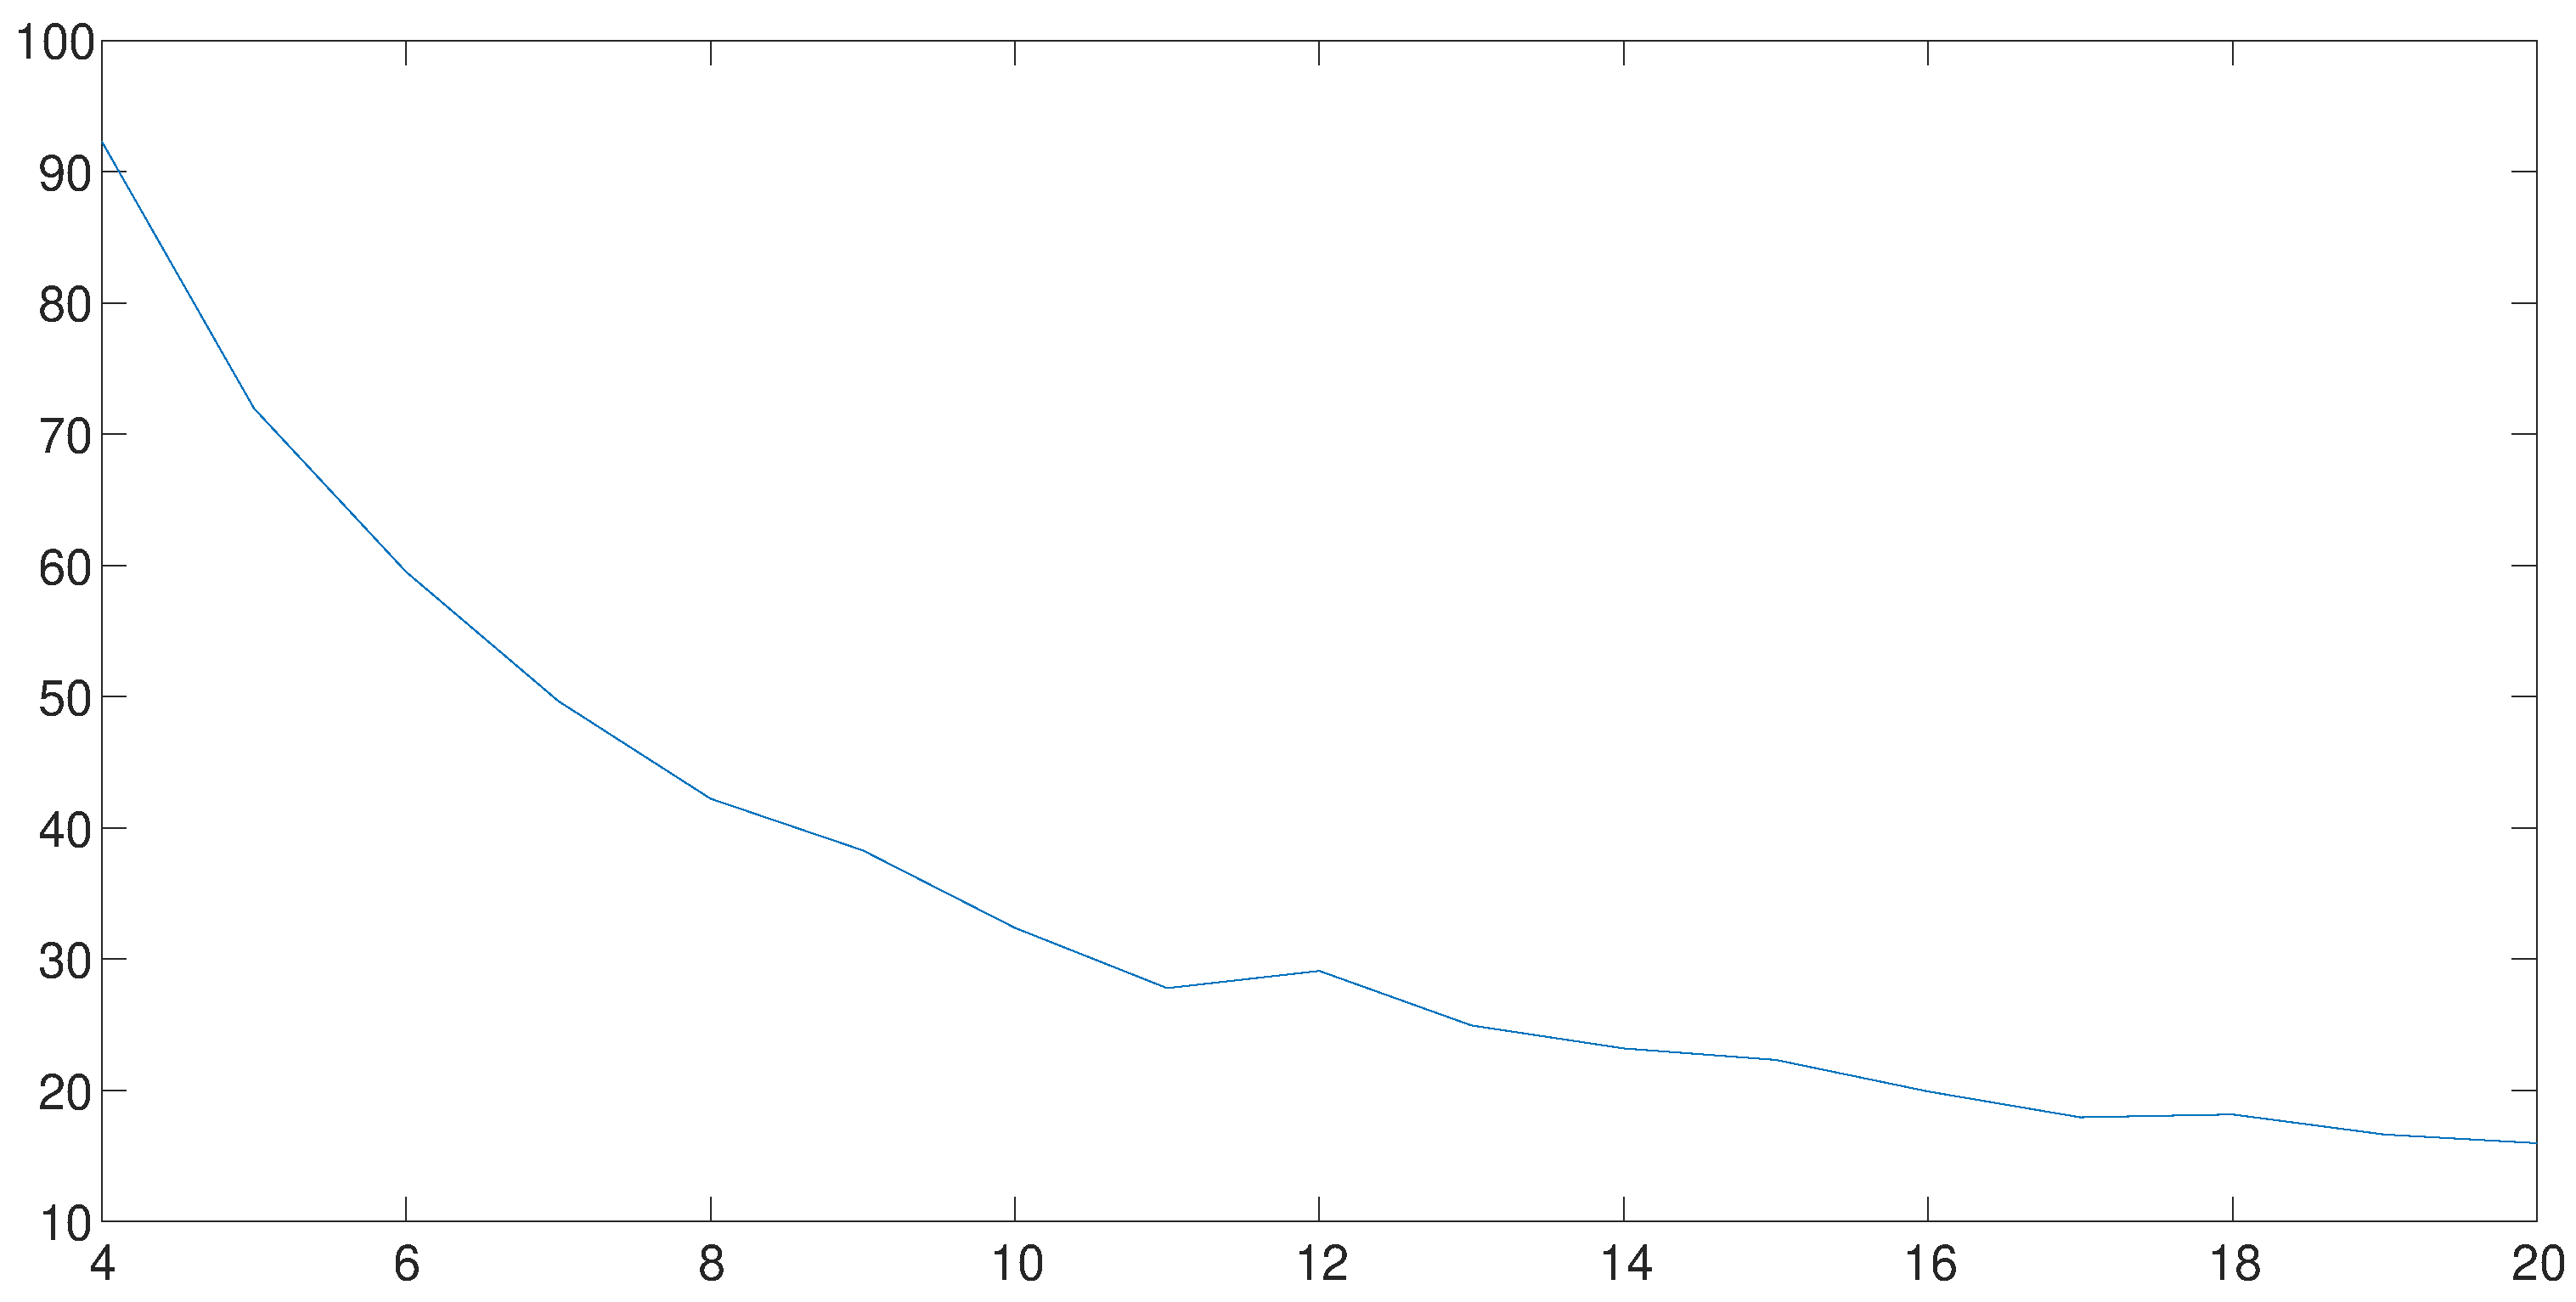
\includegraphics[width=0.9\textwidth]{images/keyrate.eps}
    \caption{不同降采样率的密钥生成速率}
    \label{keyrate}
\end{figure}


\subsection{纠错码对密钥一致率}

发送端使用随机的消息比特作为输入,利用纠错码编码,再与密钥流异或,接收端再与密钥流异或,然后利用送入纠错解码器解码。本文分别计算了9种情况下BCH码和Turbo码的纠错能力。每情况使用600组数据计算平均误码率以及平均密钥一致率。

如图\ref{bar-bch-ber-nine}为9种情况下BCH码的纠错效果,其中参数N = 31, K = 11。具体数据见表格\ref{bch-ber-nine},可以观察出密钥一致率变高,纠错之后的误比特率也会随着降低。所有场景中,密钥一致率最高为室外静态方式的95\%,其也对应着最低的误比特率7.25\%;密钥一致率最低为室内终端移动场景91.75\%,其也对应着最高的误比特率9.99\%。

如图\ref{bar-turbo-ber-nine}为9种情况下Turbo码的纠错效果,其中迭代次数为8,N = 2, K = 3,生成多项式为g = [1 1 1; 1 0 1]。所有场景中,密钥一致率最高为室外静态方式的95\%,其也对应着最低的误比特率1.43\%;密钥一致率最低为室内终端移动场景91.75\%,其对应这最高的误比特率5.29\%。相对于BCH纠错码来说,Turbo码的误比特率更小一些,因为Turbo的信道纠错性能更加接近香农极限。

\begin{figure}[htbp!]
    \centering 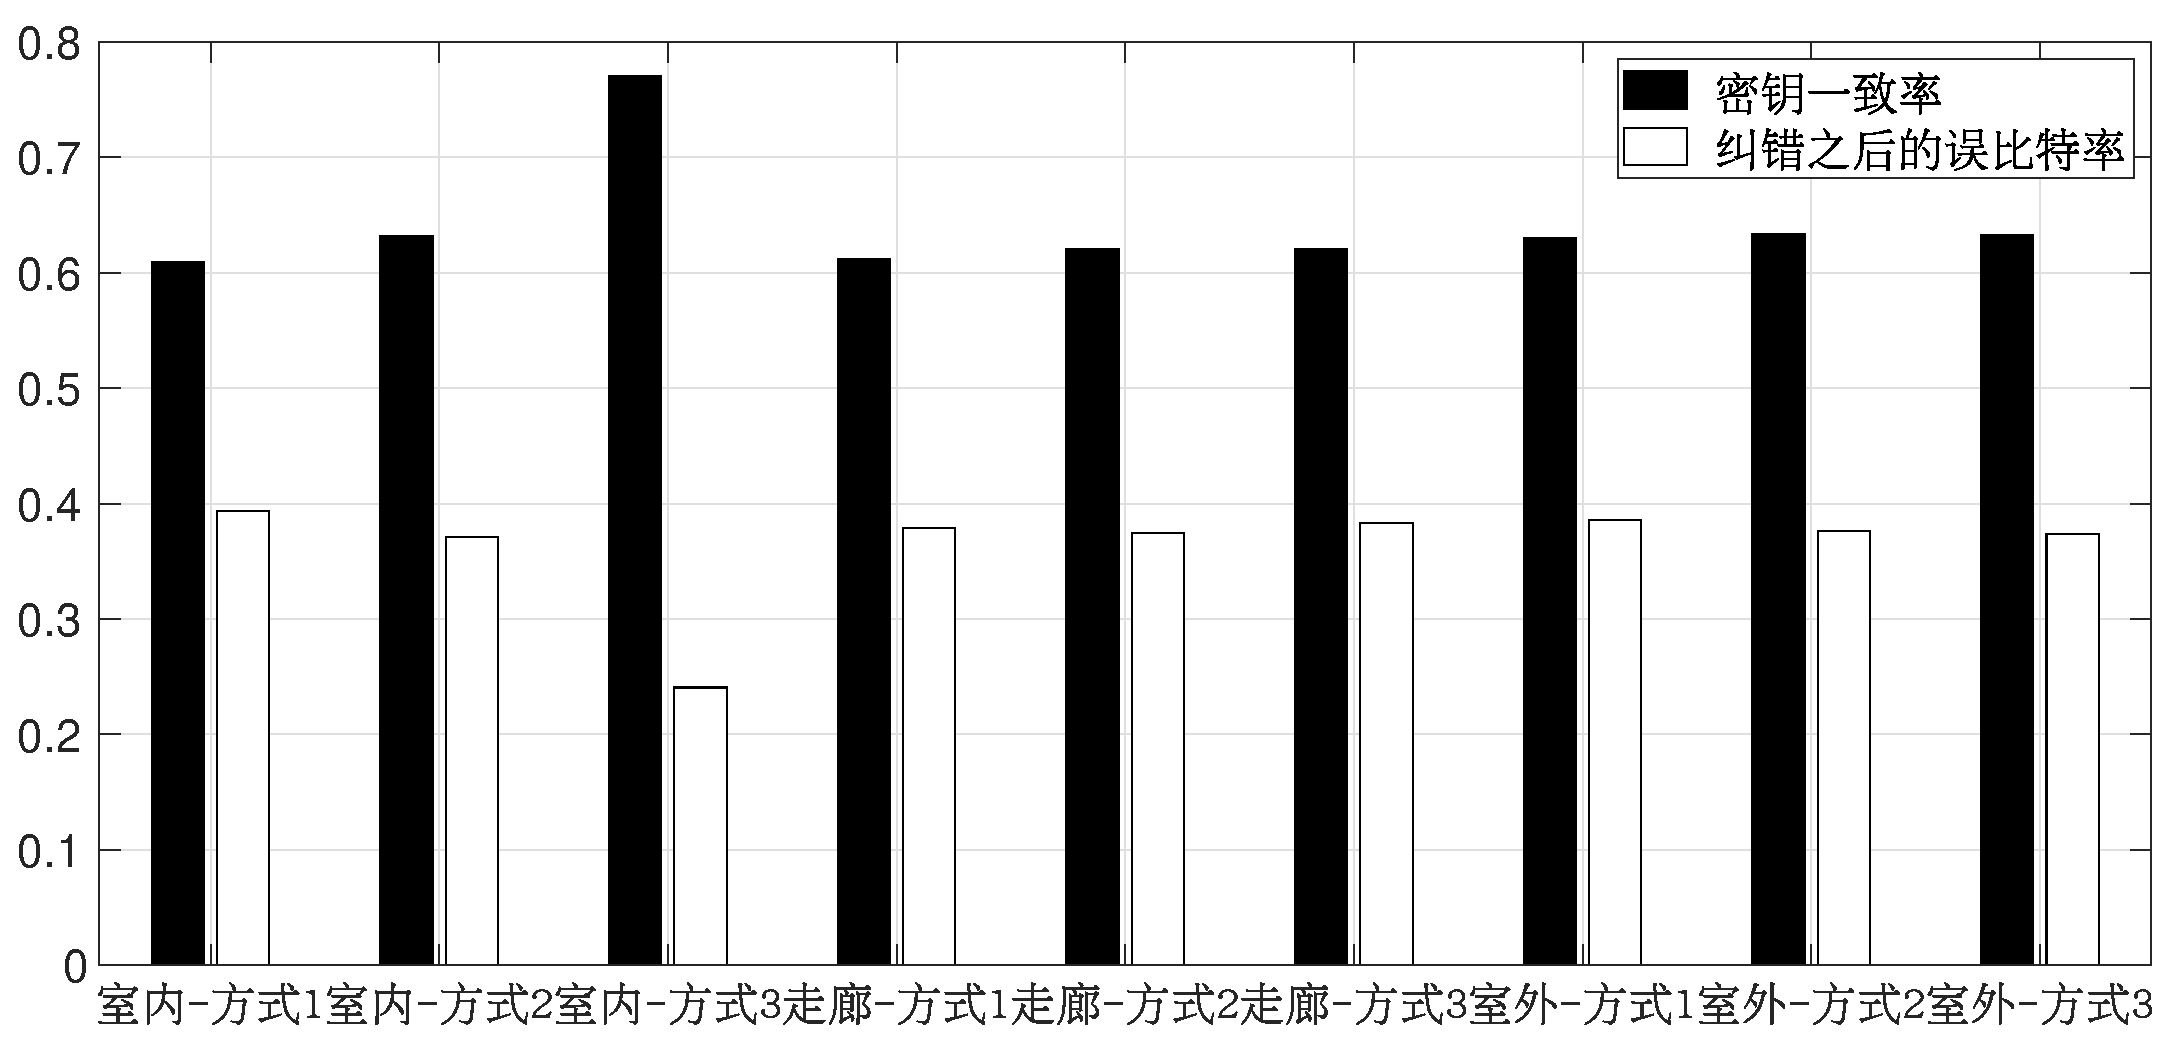
\includegraphics[width=0.9\textwidth]{images/tdd-encode/bch-ber-nine.eps}
    \caption{不同情况下BCH的平均误码率以及对应的平均密钥一致率}
    \label{bar-bch-ber-nine}
\end{figure}

\begin{table}[]
    \centering
    \setlength{\tabcolsep}{10mm}{
    \begin{tabular}{cccc} 
        \toprule
        & \textbf{方式1} & \textbf{方式2} & \textbf{方式3} \\
        \midrule
        室内 & 0.9445/0.0830 & 0.9434/0.0768 & 0.9175/0.0999 \\ 
        走廊 & 0.9296/0.0870 & 0.9413/0.0797 & 0.9362/0.0850 \\ 
        室外 & 0.9500/0.0685 & 0.9431/0.0786 & 0.9499/0.0725 \\
        \bottomrule
    \end{tabular}
    }
    \caption{不同情况下BCH的平均误码率以及对应的平均密钥一致率
    \label{bch-ber-nine}}
\end{table}

\begin{figure}[htbp!]
    \centering 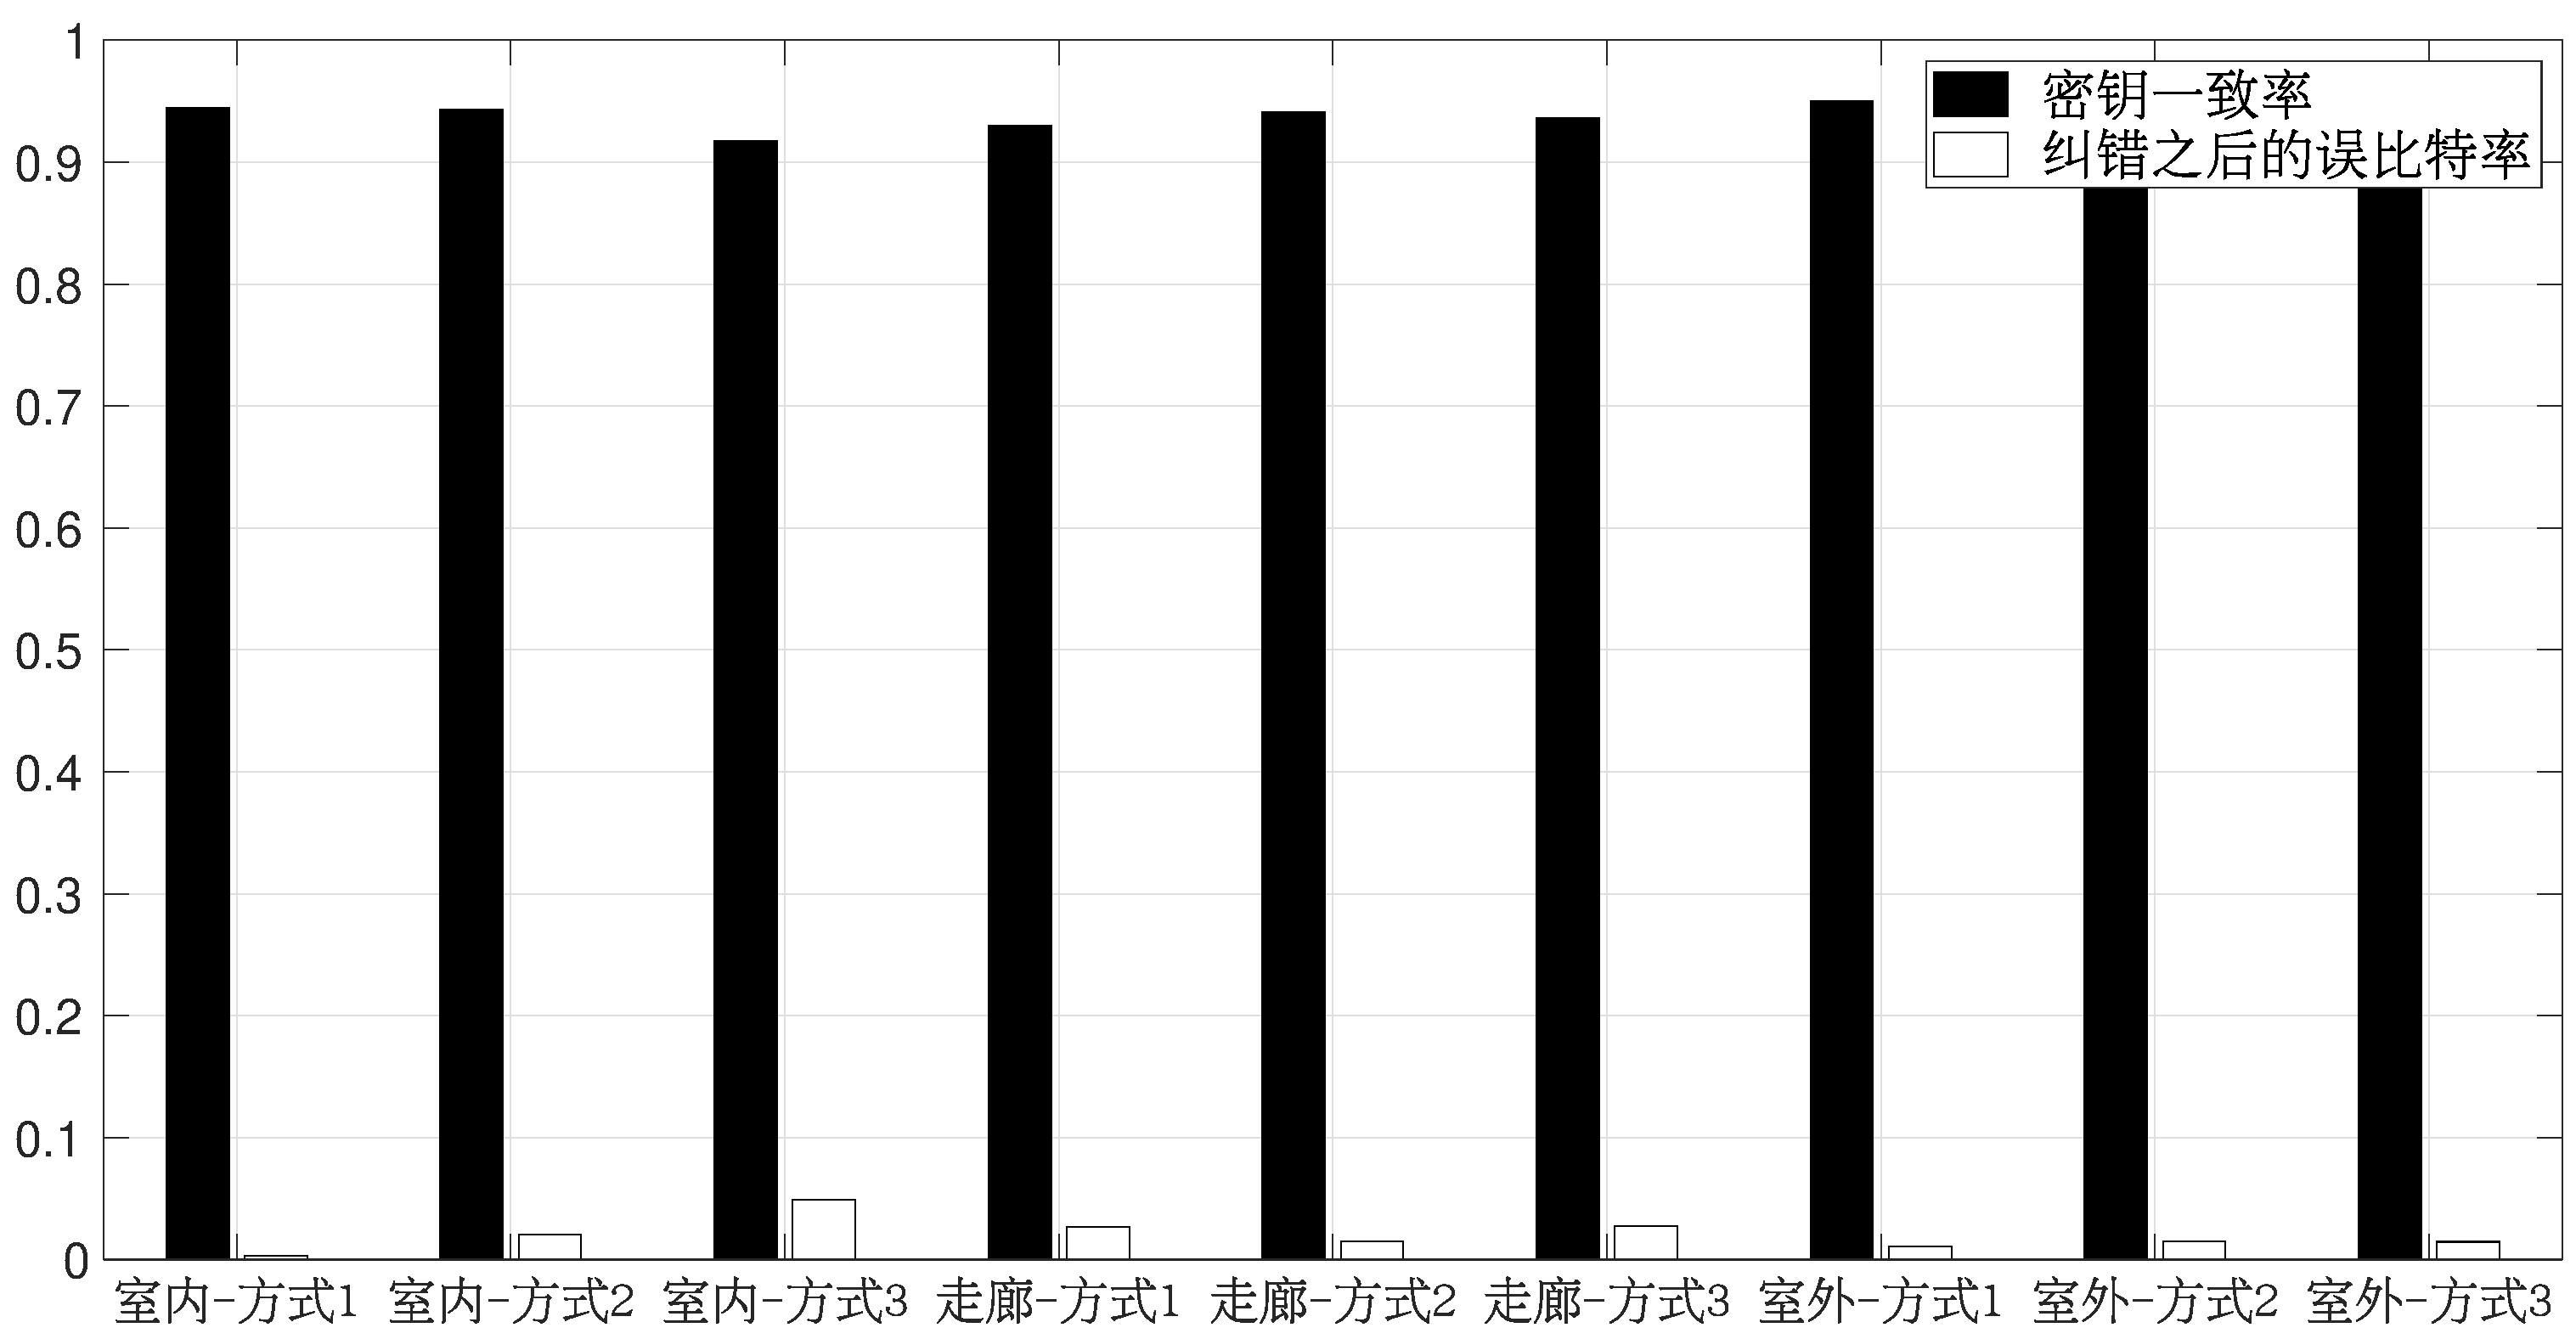
\includegraphics[width=0.9\textwidth]{images/tdd-encode/turbo-ber-nine.eps}
    \caption{不同情况下Turbo的平均误码率以及对应的平均密钥一致率}
    \label{bar-turbo-ber-nine}
\end{figure}


\begin{table}[]
    \centering
    \setlength{\tabcolsep}{10mm}{
    \begin{tabular}{cccc} 
        \toprule
        & \textbf{方式1} & \textbf{方式2} & \textbf{方式3} \\
        \midrule
        室内 & 0.9445/0.0146 & 0.9434/0.0262 & 0.9175/0.0529 \\ 
        走廊 & 0.9296/0.0378 & 0.9413/0.0188 & 0.9362/0.0301 \\ 
        室外 & 0.9500/0.0143 & 0.9431/0.0180 & 0.9499/0.0157 \\
        \bottomrule
    \end{tabular}
    }
    \caption{不同情况下Turbo的平均误码率以及对应的平均密钥一致率
    \label{turbo-ber-nine}}
\end{table}


\section{FDD模式}

与TDD相似,本文同样在FDD模式下的9种情况中,连续各采集600组数据,并计算相应指标。FDD模式下的实验参数如表\ref{fdd-exp-args}所示,导频信号中正弦波的频率、M序列长度与TDD模式相同。USRP采样率设置为25MHz。与TDD模式不同的是,FDD的上下行频率分别是2535MHz和2595MHz。本文计算了Alice在三个场景、三种信道环境的600组CSI,结果如图\ref{fdd_csi_ab}所示。图中x轴是测量次数,y轴是子载波数,z轴是幅度值,即从时间的维度来观察CSI的变化。

从CSI图示结果中可以看出,在所有场景中,室内房间终端固定的情况下,CSI最为稳定;空旷室外终端移动的情况下,CSI变化最快。在室内、走廊和室外三种场景中,室内房间的CSI最为稳定,走廊和室外的CSI变化相对更大。在终端固定、人员移动和终端移动三种信道环境中,终端固定的CSI变化最慢;终端移动时CSI变化最快。

和TDD一样,本文接下来将计算多个指标,分析无线密钥生成系统在FDD模式下的可靠性和安全性。

\begin{table}[]
    \centering
    \begin{tabular}{|l|l|l|l|}
    \hline
    \multicolumn{2}{|c|}{参数} & Alice & Bob \\ \hline
    \multirow{6}{*}{USRP} & 发射载波频率(MHz) & 2535 & 2595 \\ \cline{2-4} 
     & 接收载波频率(MHz) & 2595 & 2535 \\ \cline{2-4} 
     & 采样率(MHz) & 25 & 25 \\ \cline{2-4} 
     & 增益(dB) & 30 & 30 \\ \cline{2-4} 
     & 天线 & Tx/Rx & Tx/Rx \\ \cline{2-4} 
     & 带宽(MHz) & 20 & 20 \\ \hline
    \multirow{4}{*}{导频信号} & 正弦波长度 & 1504 & 1504 \\ \cline{2-4} 
     & 正弦波频率(Hz) & 4 & 8 \\ \cline{2-4} 
     & M序列长度 & 4095 & 4095 \\ \cline{2-4} 
     & CP循环前缀长度 & 129 & 129 \\ \hline
    \end{tabular}
    \caption{FDD模式下的实验参数
    \label{fdd-exp-args}}
\end{table}

\begin{figure}
    \centering
    \subfigure[室内-方式1]{
        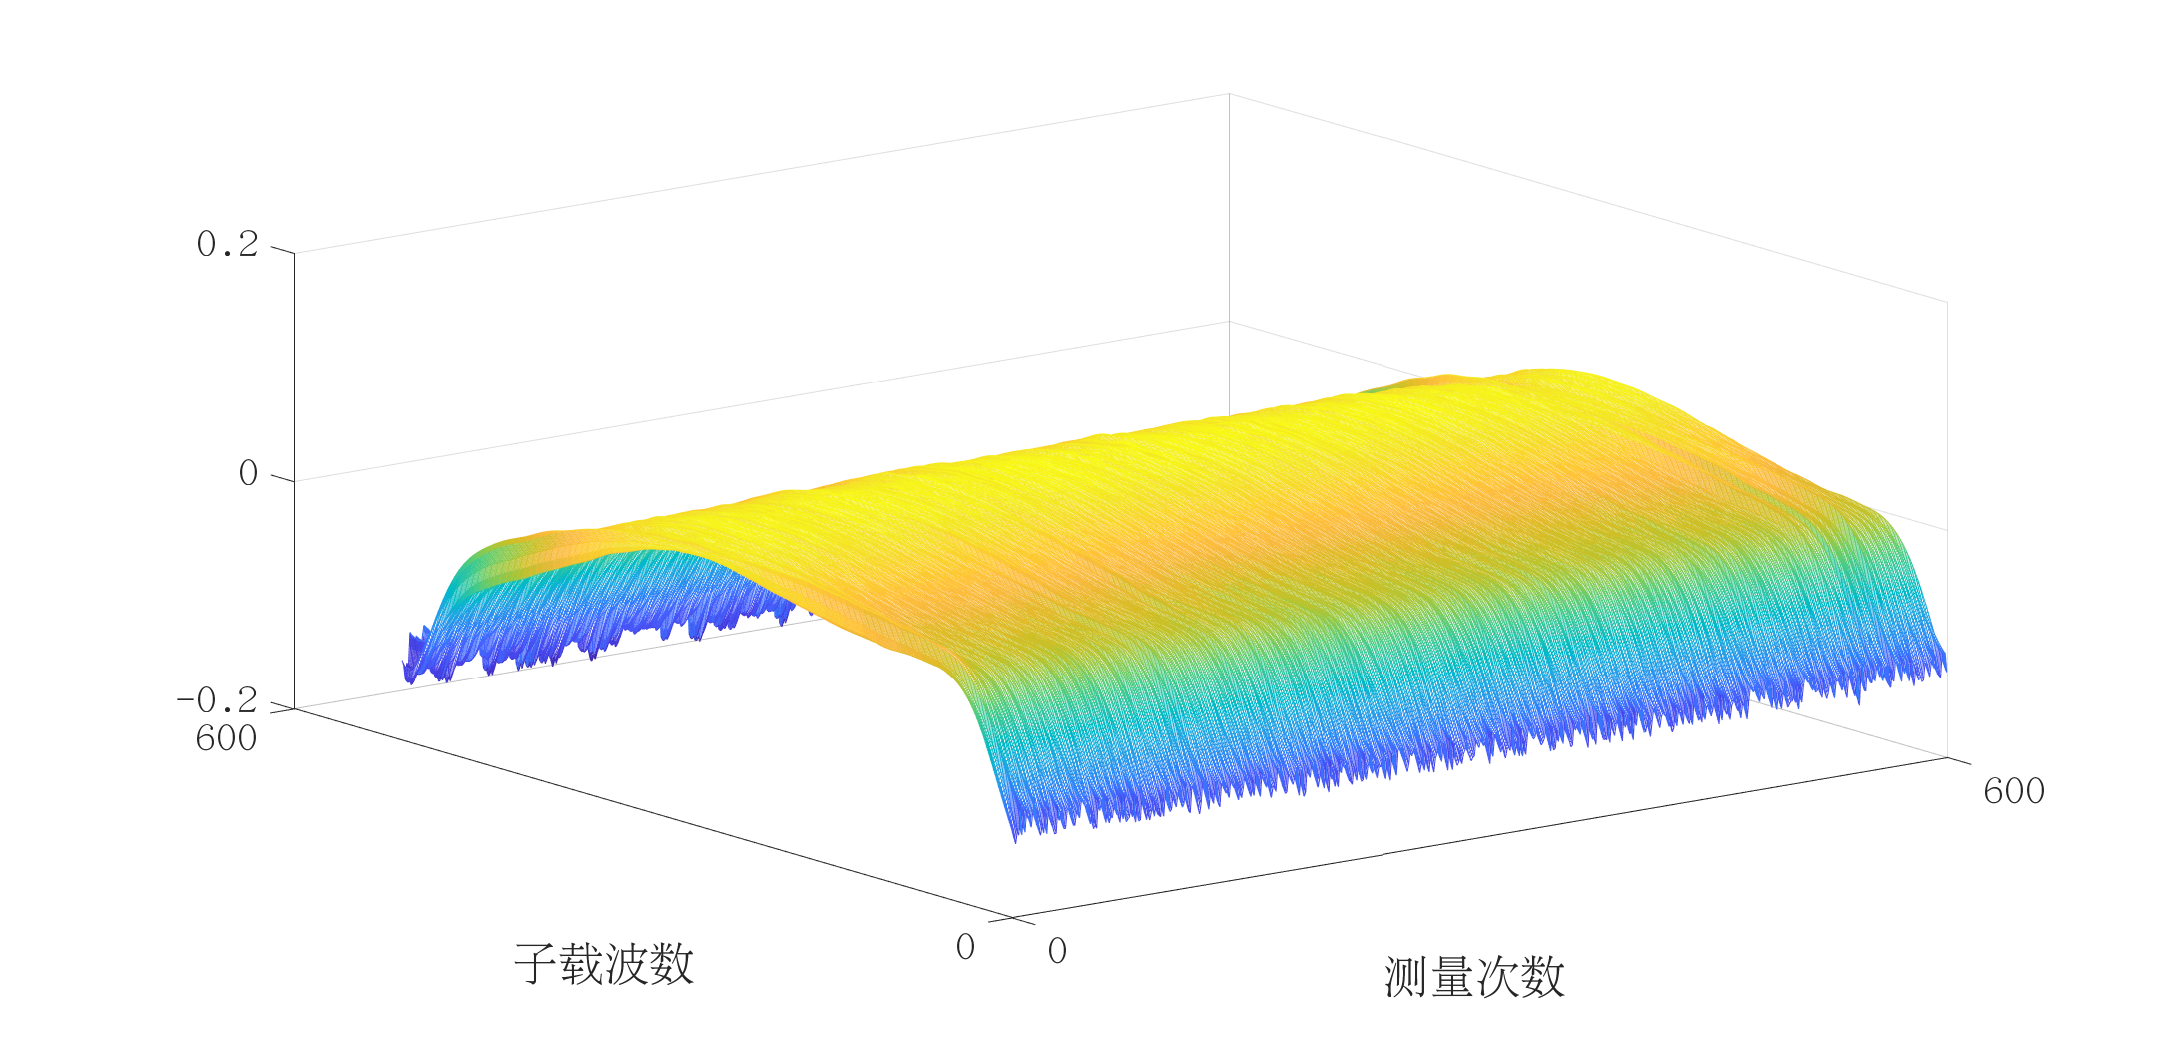
\includegraphics[width=0.3\textwidth]{images/fdd-csi/indoor-no-move.eps}
    }
    \subfigure[室内-方式2]{
        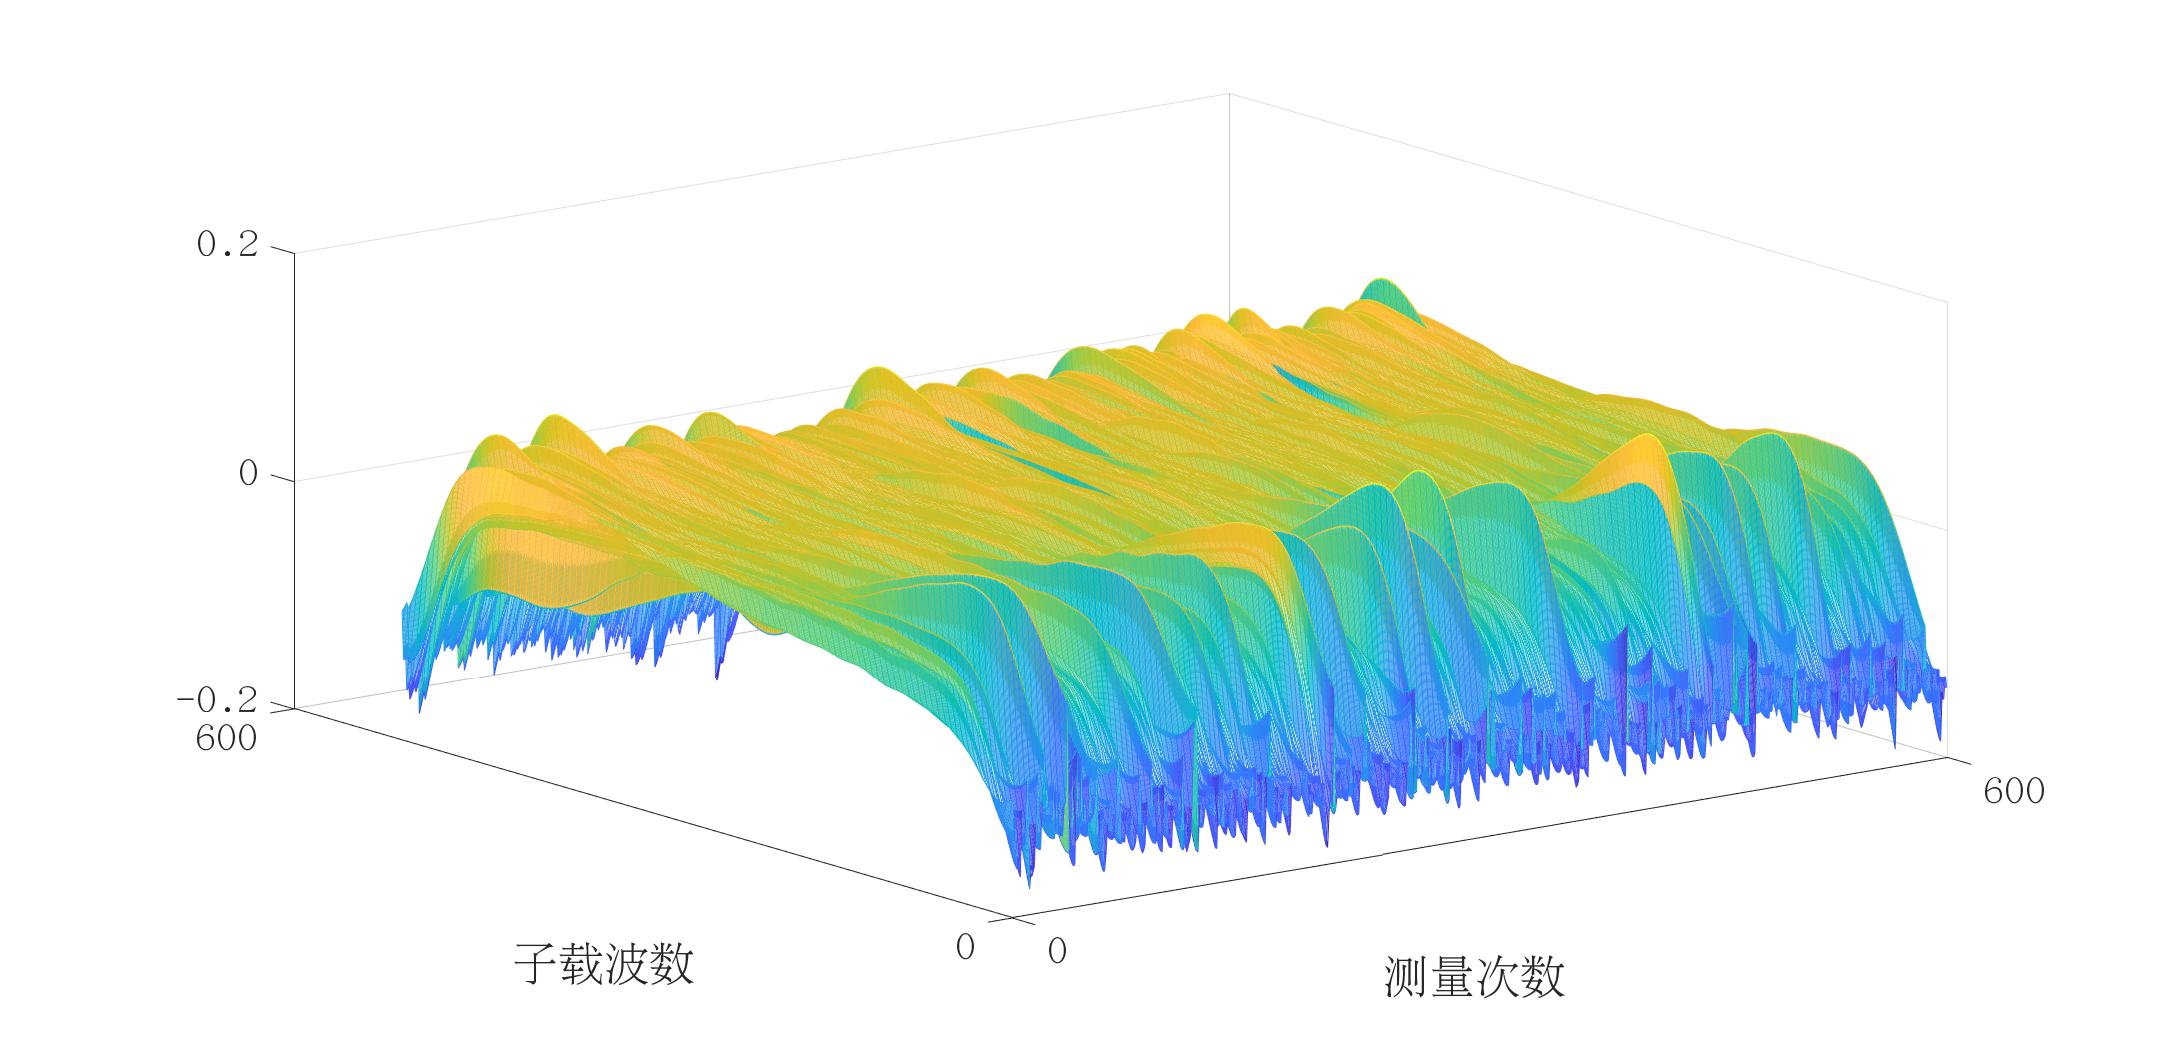
\includegraphics[width=0.3\textwidth]{images/fdd-csi/indoor-people-move.eps}
    }
    \subfigure[室内-方式3]{
        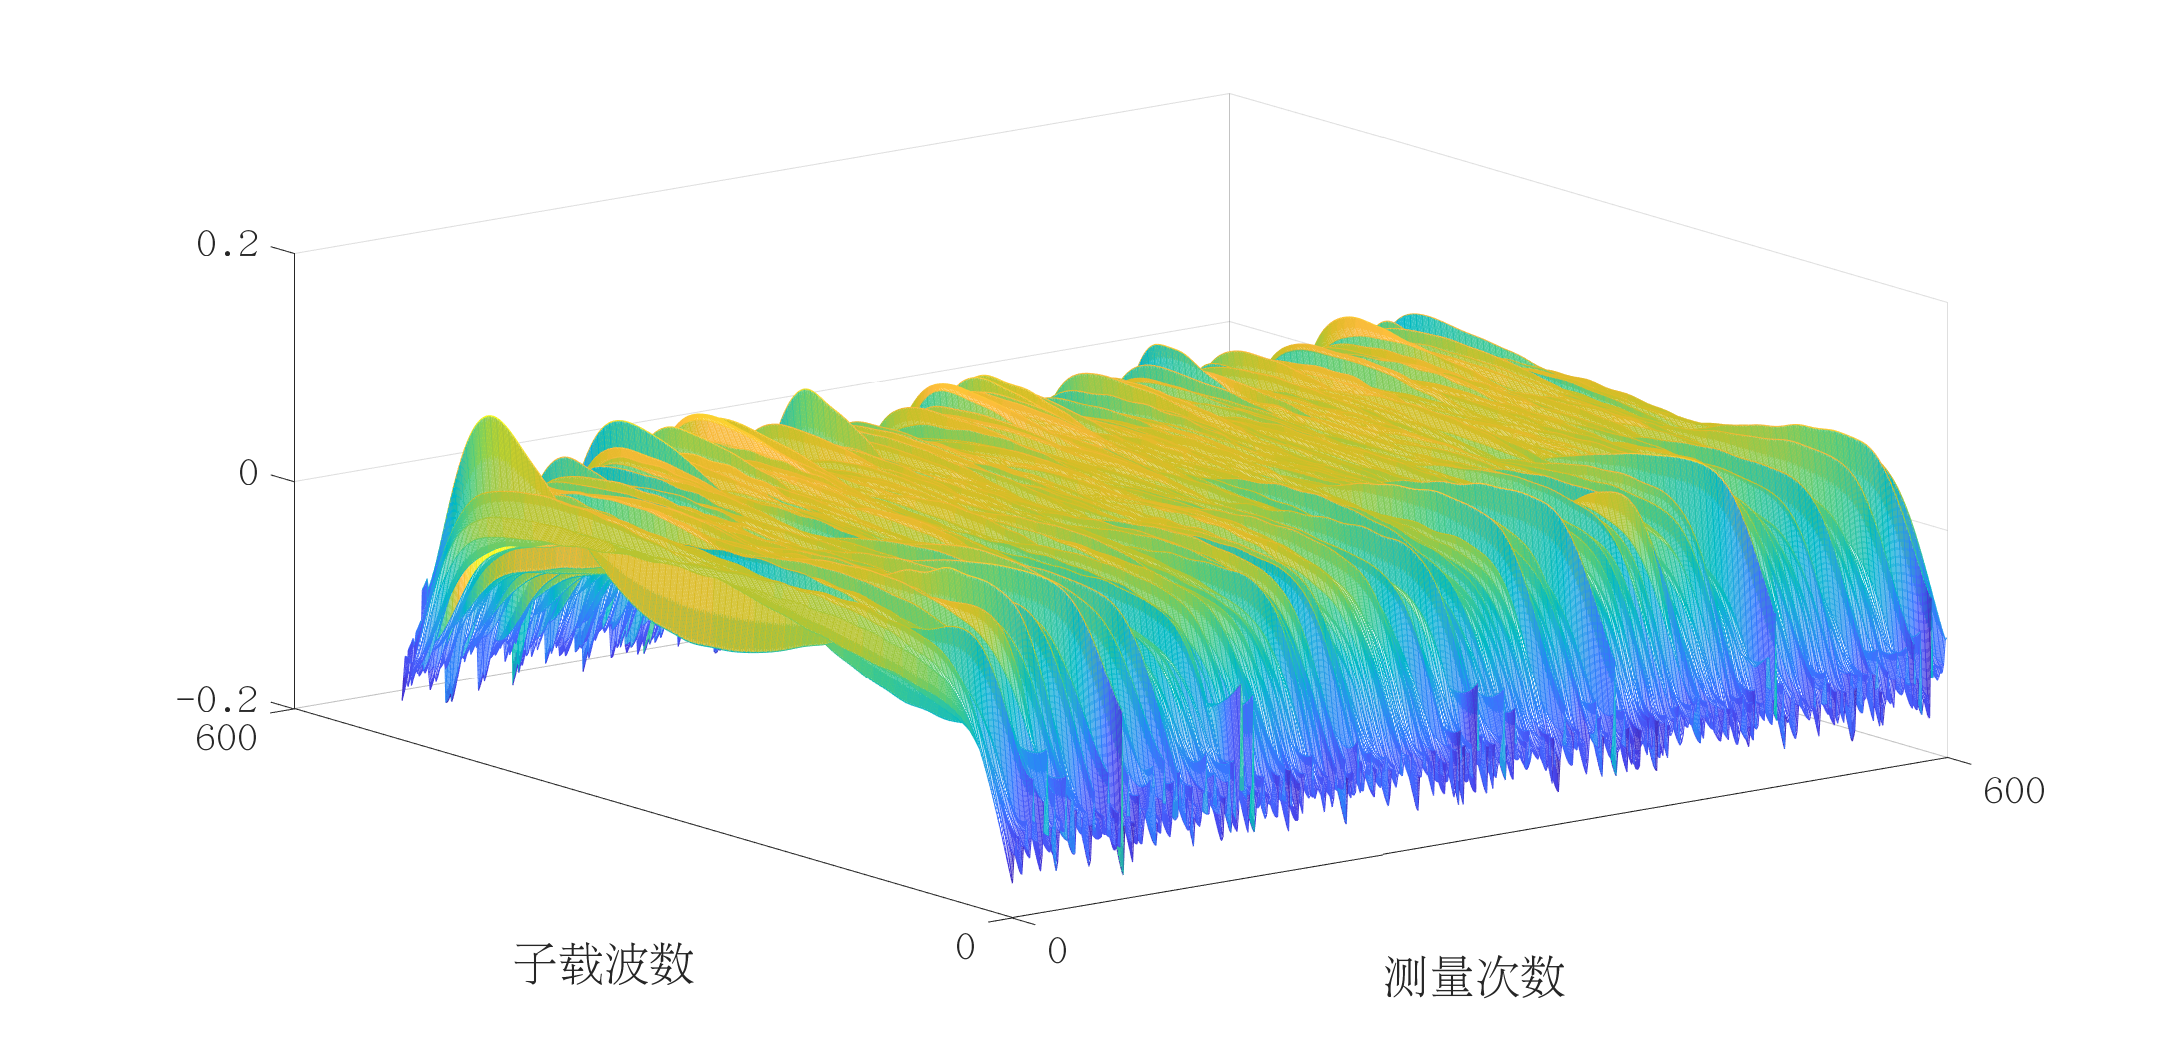
\includegraphics[width=0.3\textwidth]{images/fdd-csi/indoor-trolly-move.eps}
    }
    \quad    %用 \quad 来换行
    \subfigure[走廊-方式1]{
        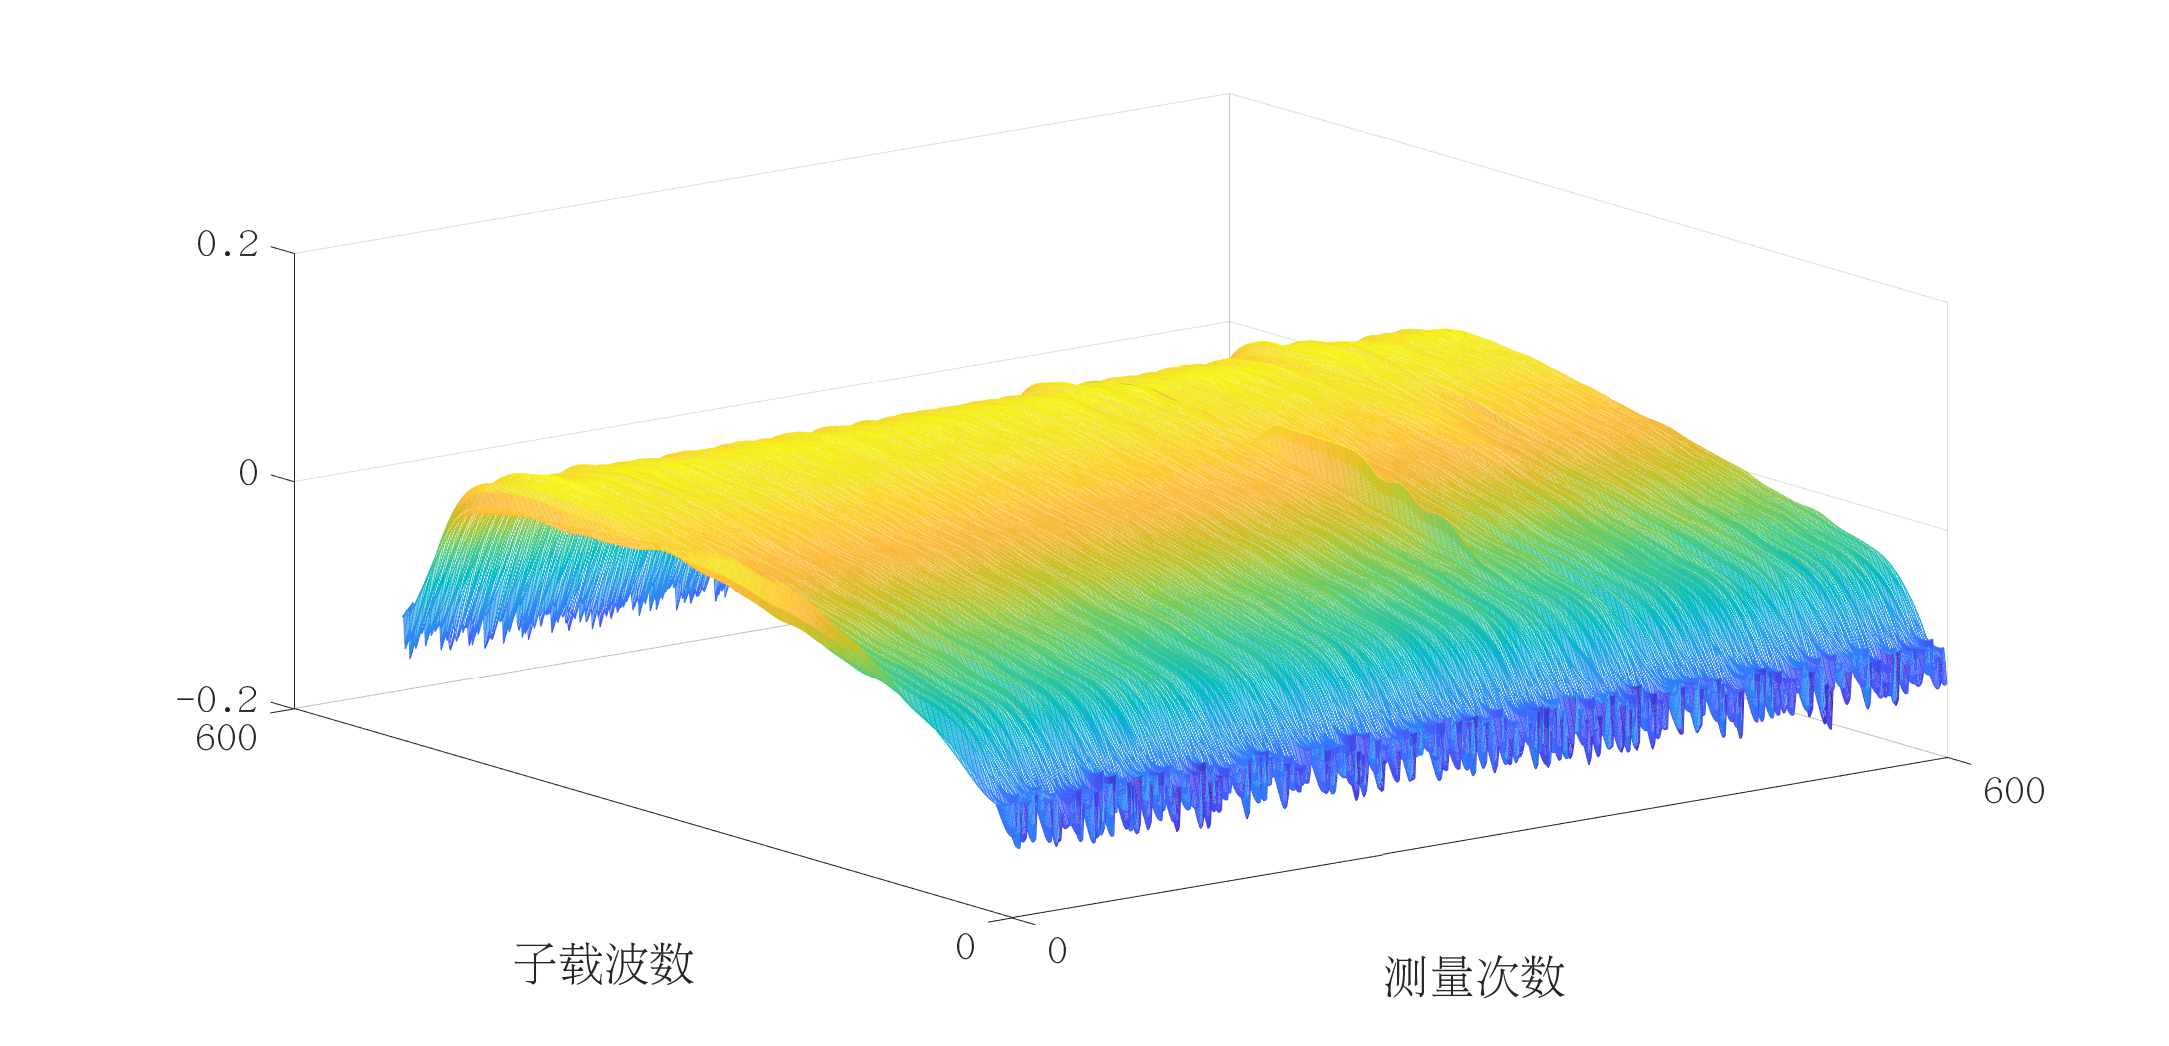
\includegraphics[width=0.3\textwidth]{images/fdd-csi/corridor-no-move.eps}
    }
    \subfigure[走廊-方式2]{
        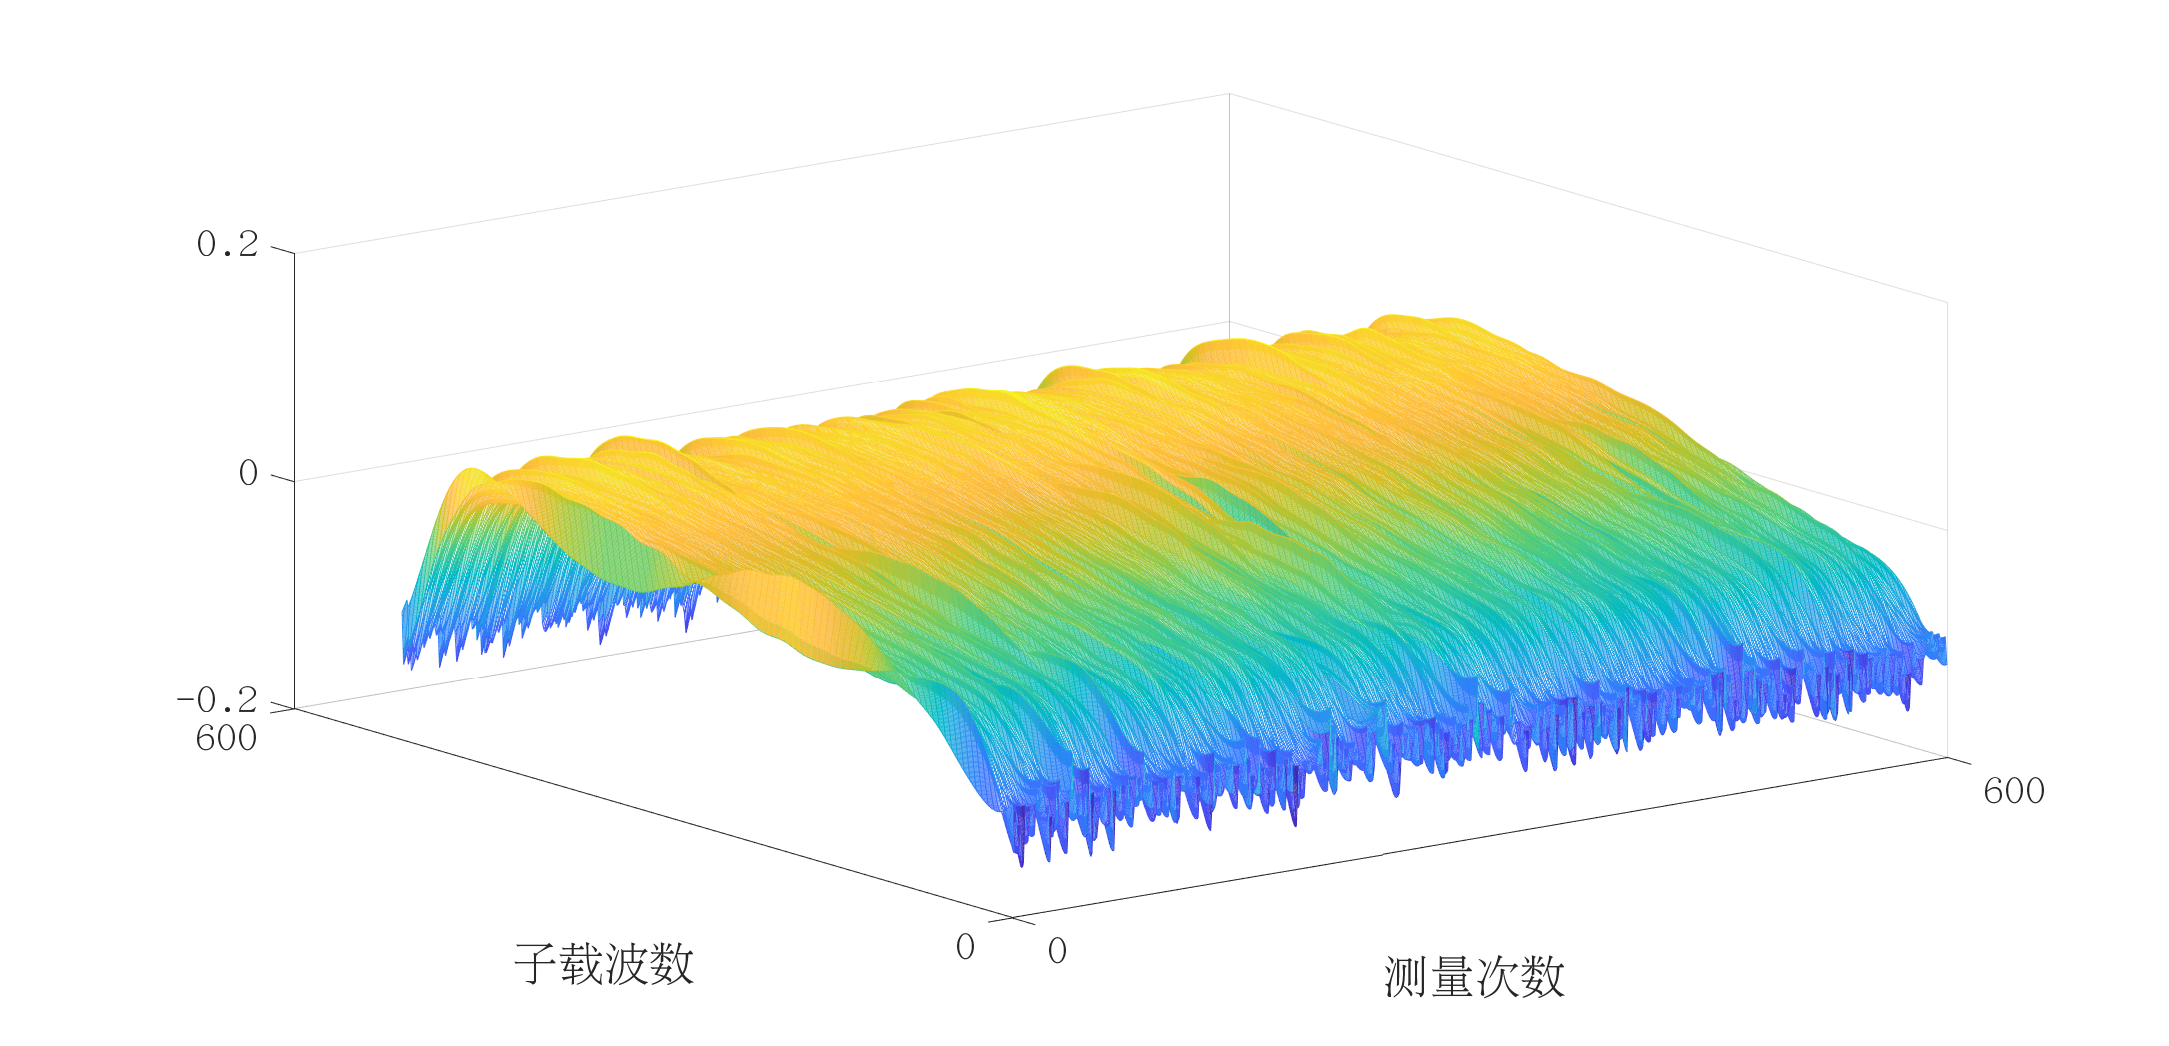
\includegraphics[width=0.3\textwidth]{images/fdd-csi/corridor-people-move.eps}
    }
    \subfigure[走廊-方式3]{
        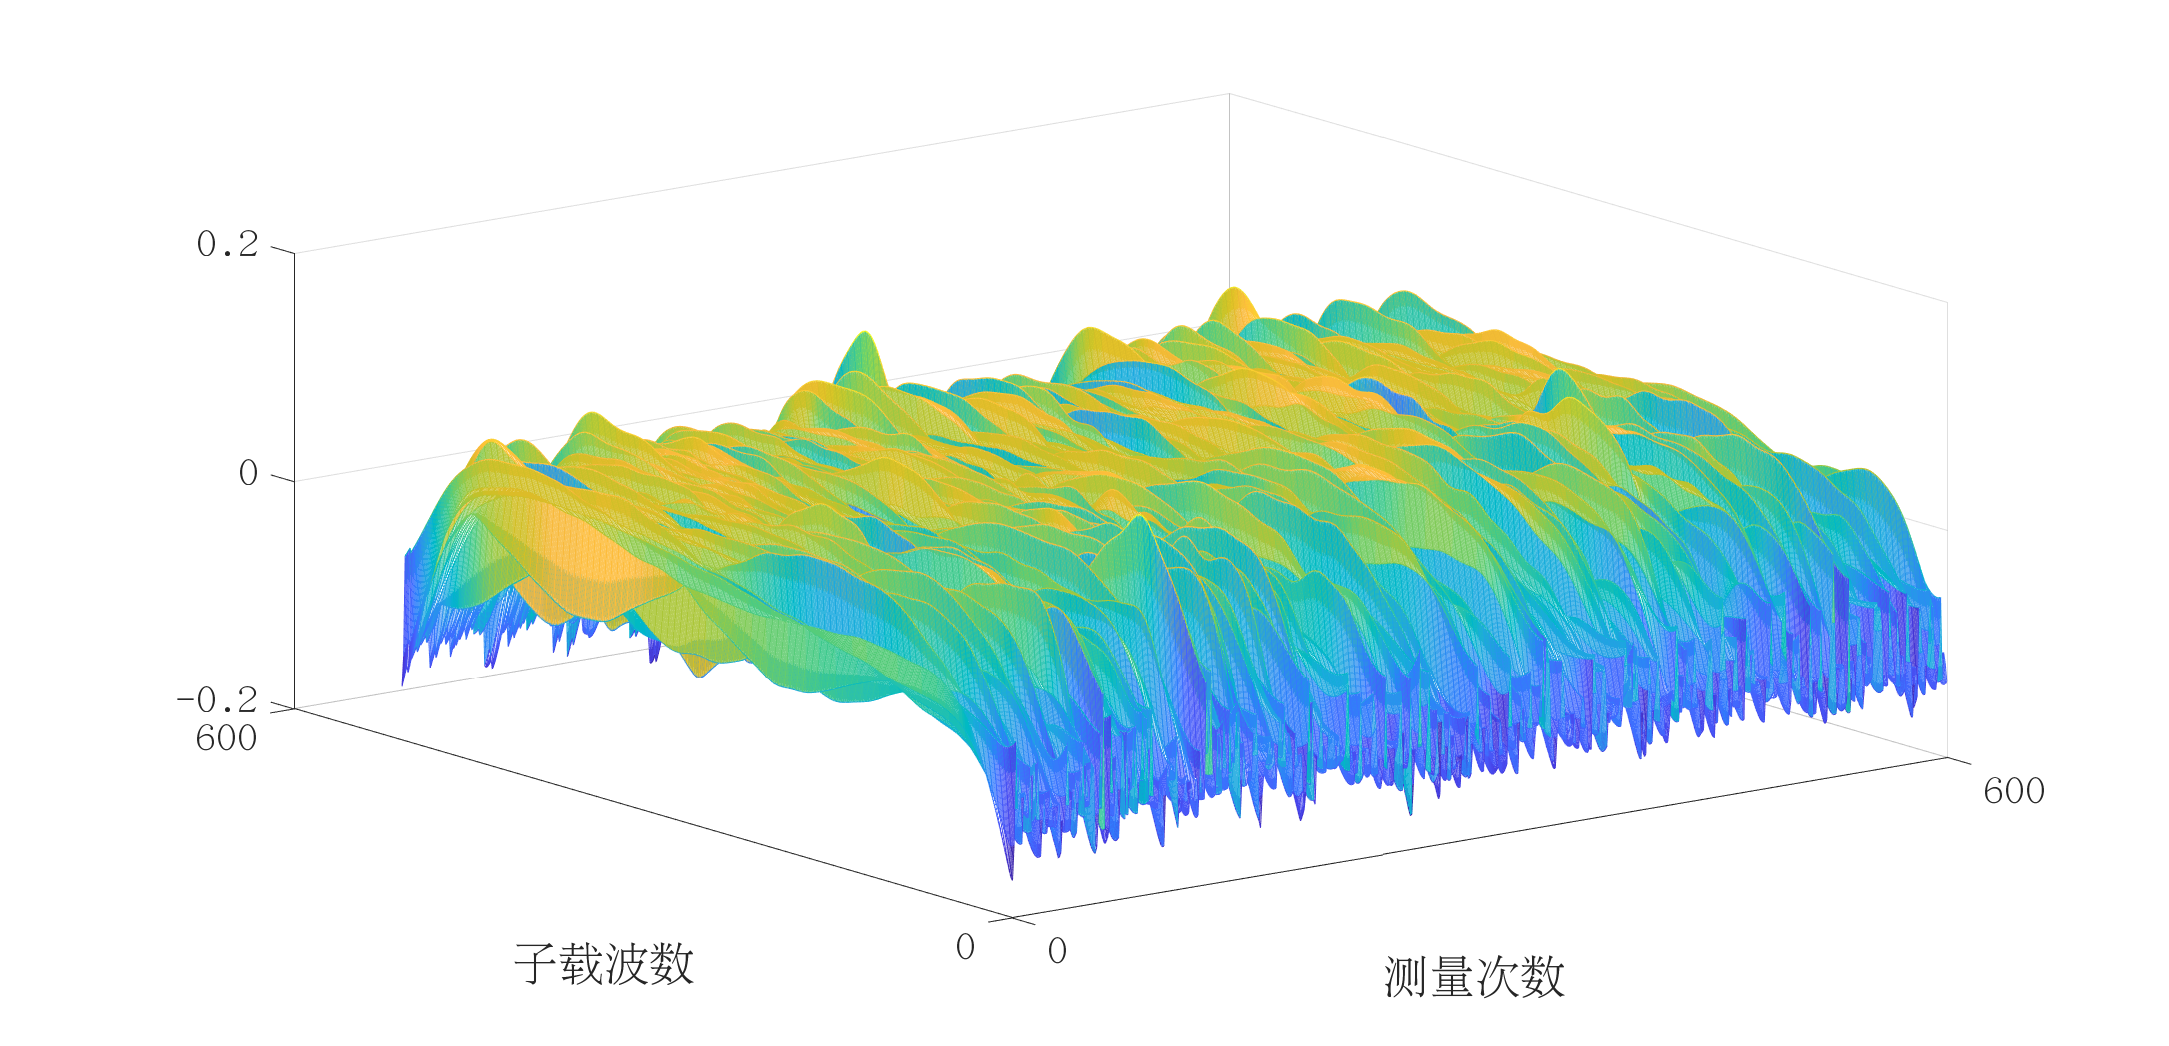
\includegraphics[width=0.3\textwidth]{images/fdd-csi/corridor-trolly-move.eps}
    }
    \quad
    \subfigure[室外-方式1]{
        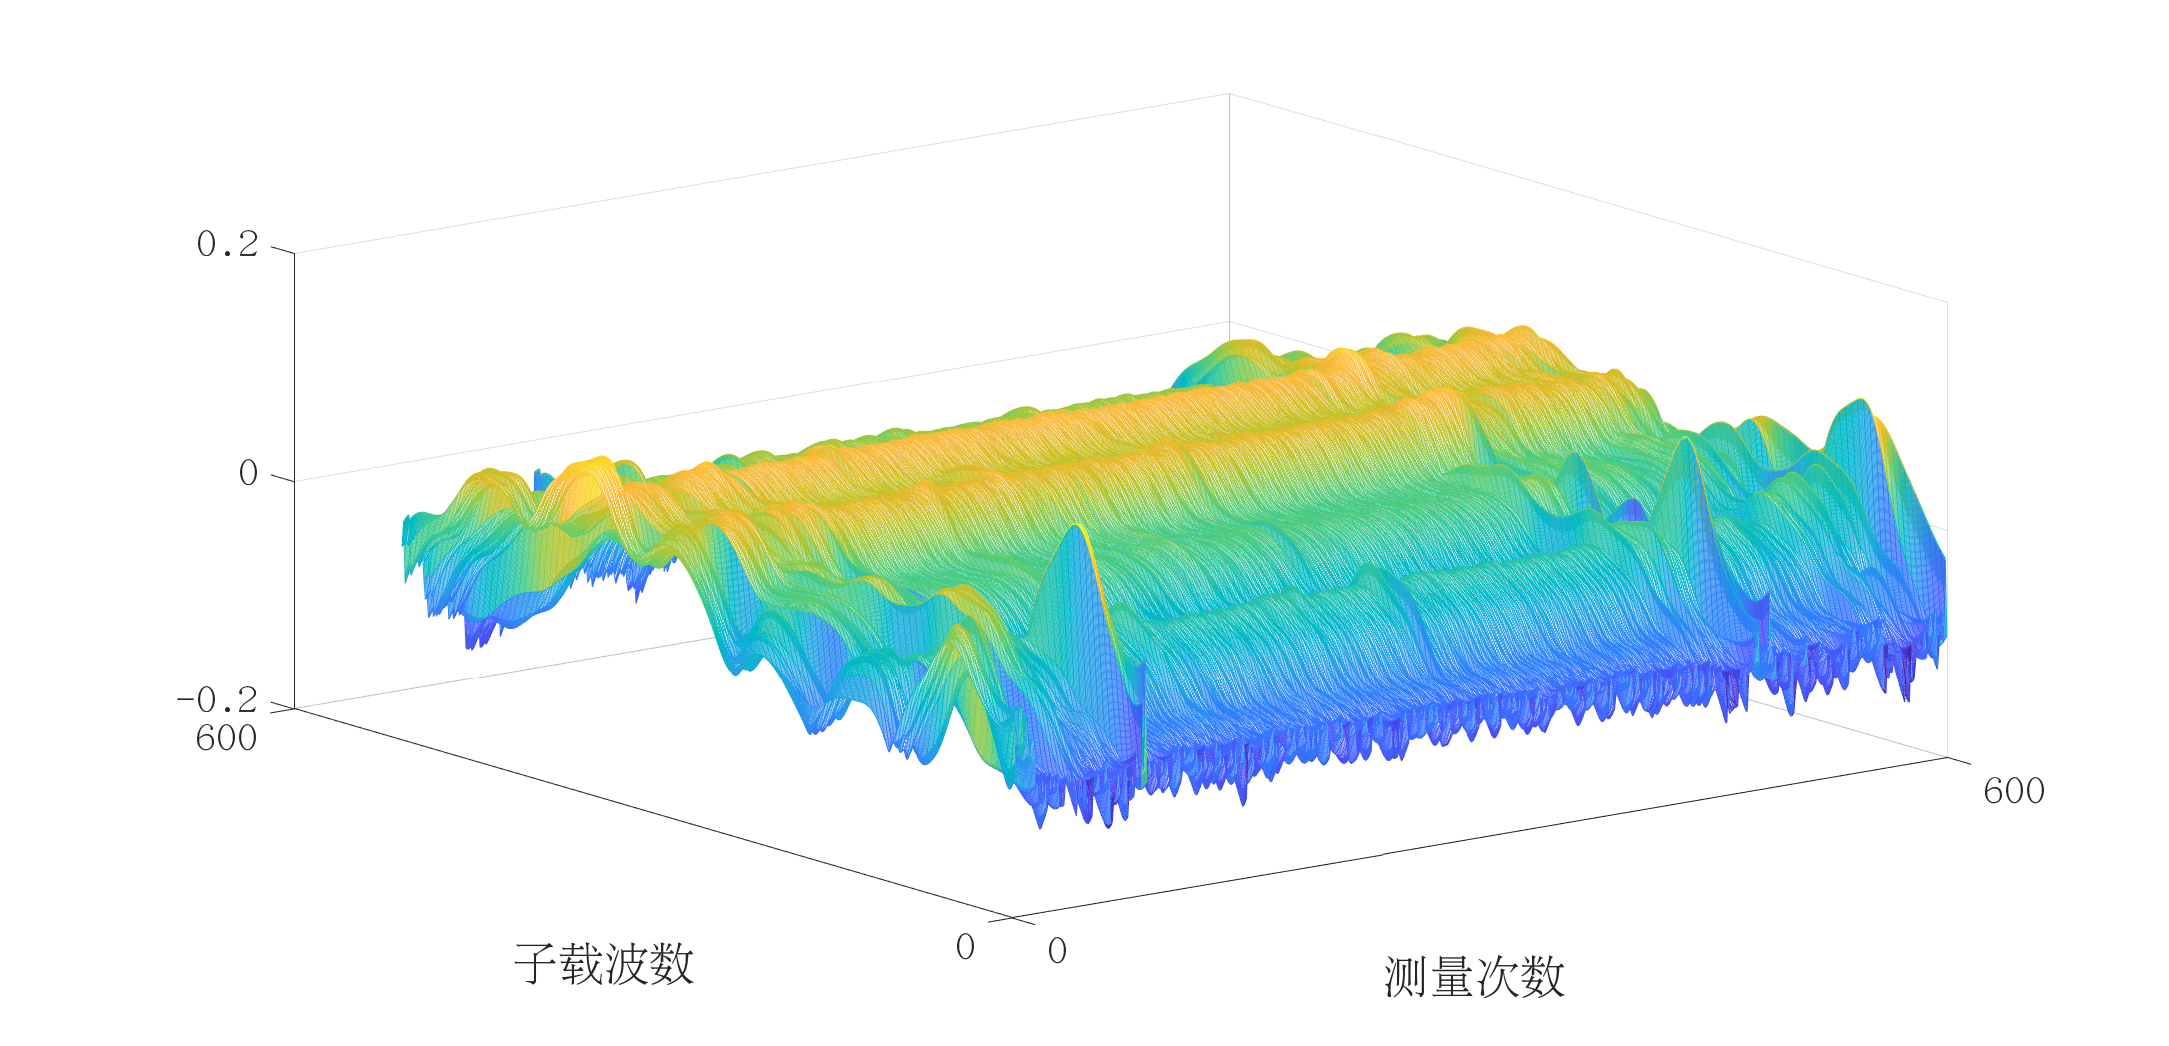
\includegraphics[width=0.3\textwidth]{images/fdd-csi/outdoor-no-move.eps}
    }
    \subfigure[室外-方式2]{
        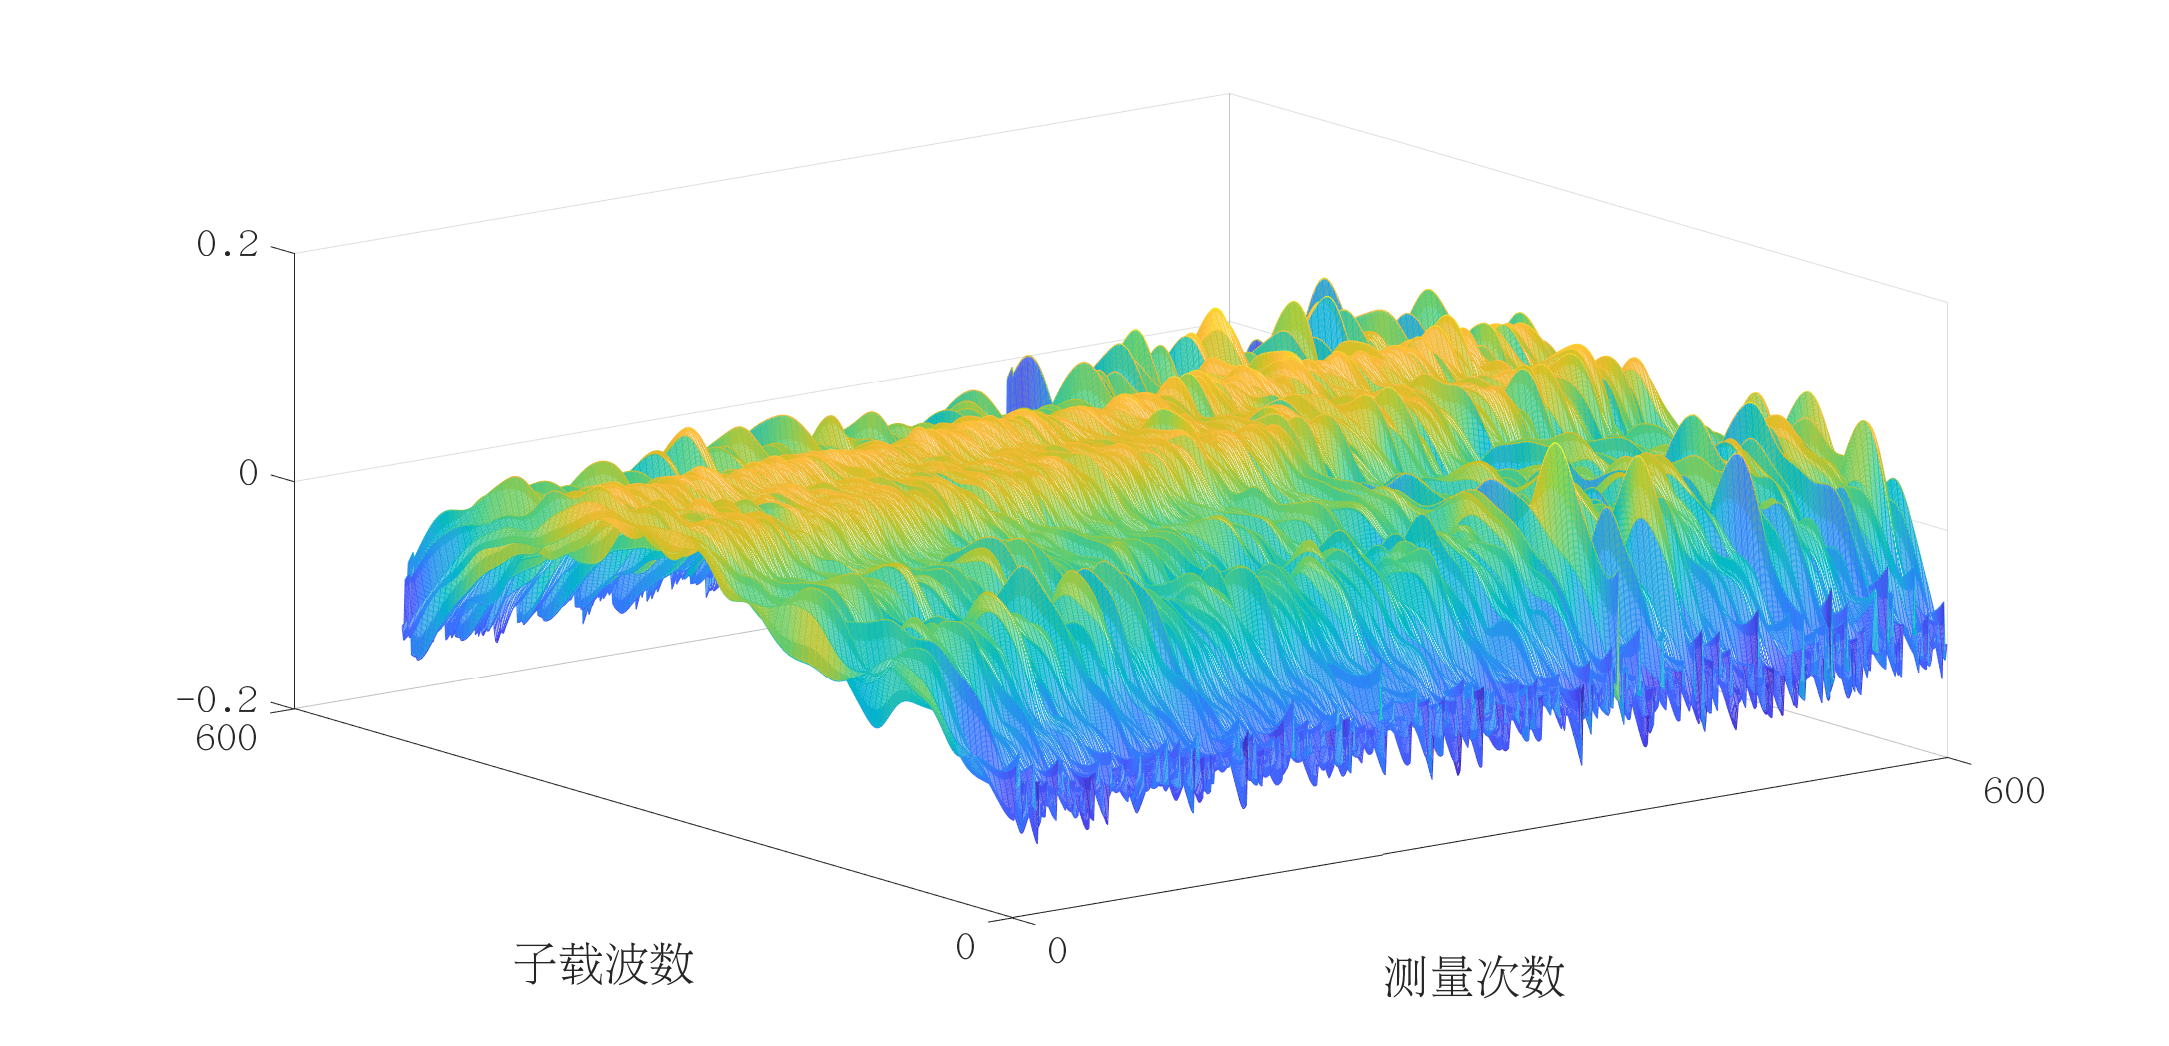
\includegraphics[width=0.3\textwidth]{images/fdd-csi/outdoor-people-move.eps}
    }
    \subfigure[室外-方式3]{
        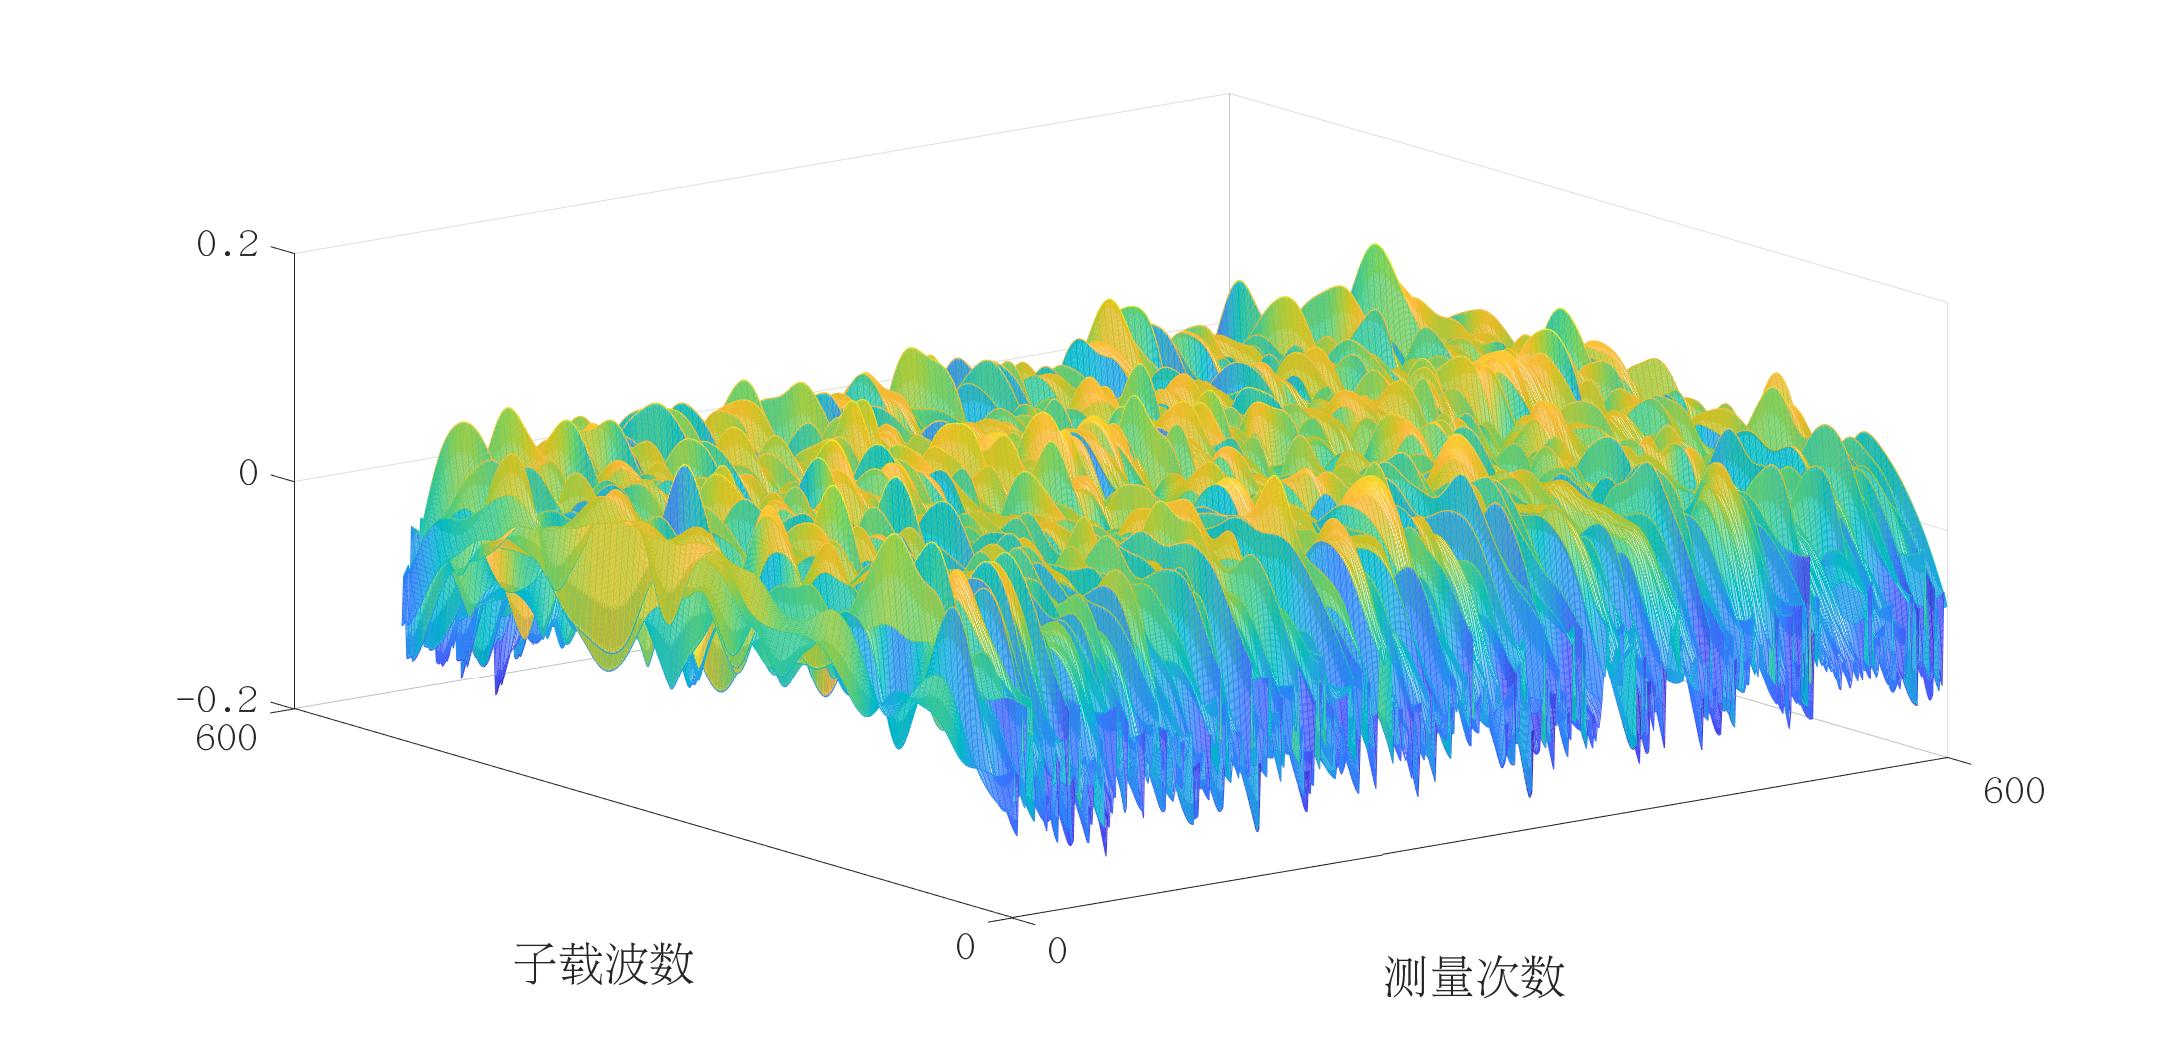
\includegraphics[width=0.3\textwidth]{images/fdd-csi/outdoor-trolly-move.eps}
    }
    \caption{不同场景与环境下CSI结果展示}{} % xcorr between alice and bob, xcorr between bob and eve
    \label{fdd_csi_ab}
\end{figure}

\subsection{CSI相关性}

理论上,FDD模式下合法通信双方的CSI相关性较差于TDD模式。本文计算FDD模式下Alice和Bob之间CSI的皮尔逊相关系数、Alice和Eve之间CSI的皮尔逊相关系数,9种情况下的结果如图\ref{fdd_csi_xcorr}所示。其中蓝色表示Alice和Bob之间CSI的皮尔逊相关系数,红色表示Alice和Eve之间CSI的皮尔逊相关系数。相对于TDD模式,FDD模式下合法通信双方的互相关系数较差,甚至在室内-方式3出现了弱于窃听者的情况。

\begin{figure}
    \centering
    \subfigure[室内-方式1]{
        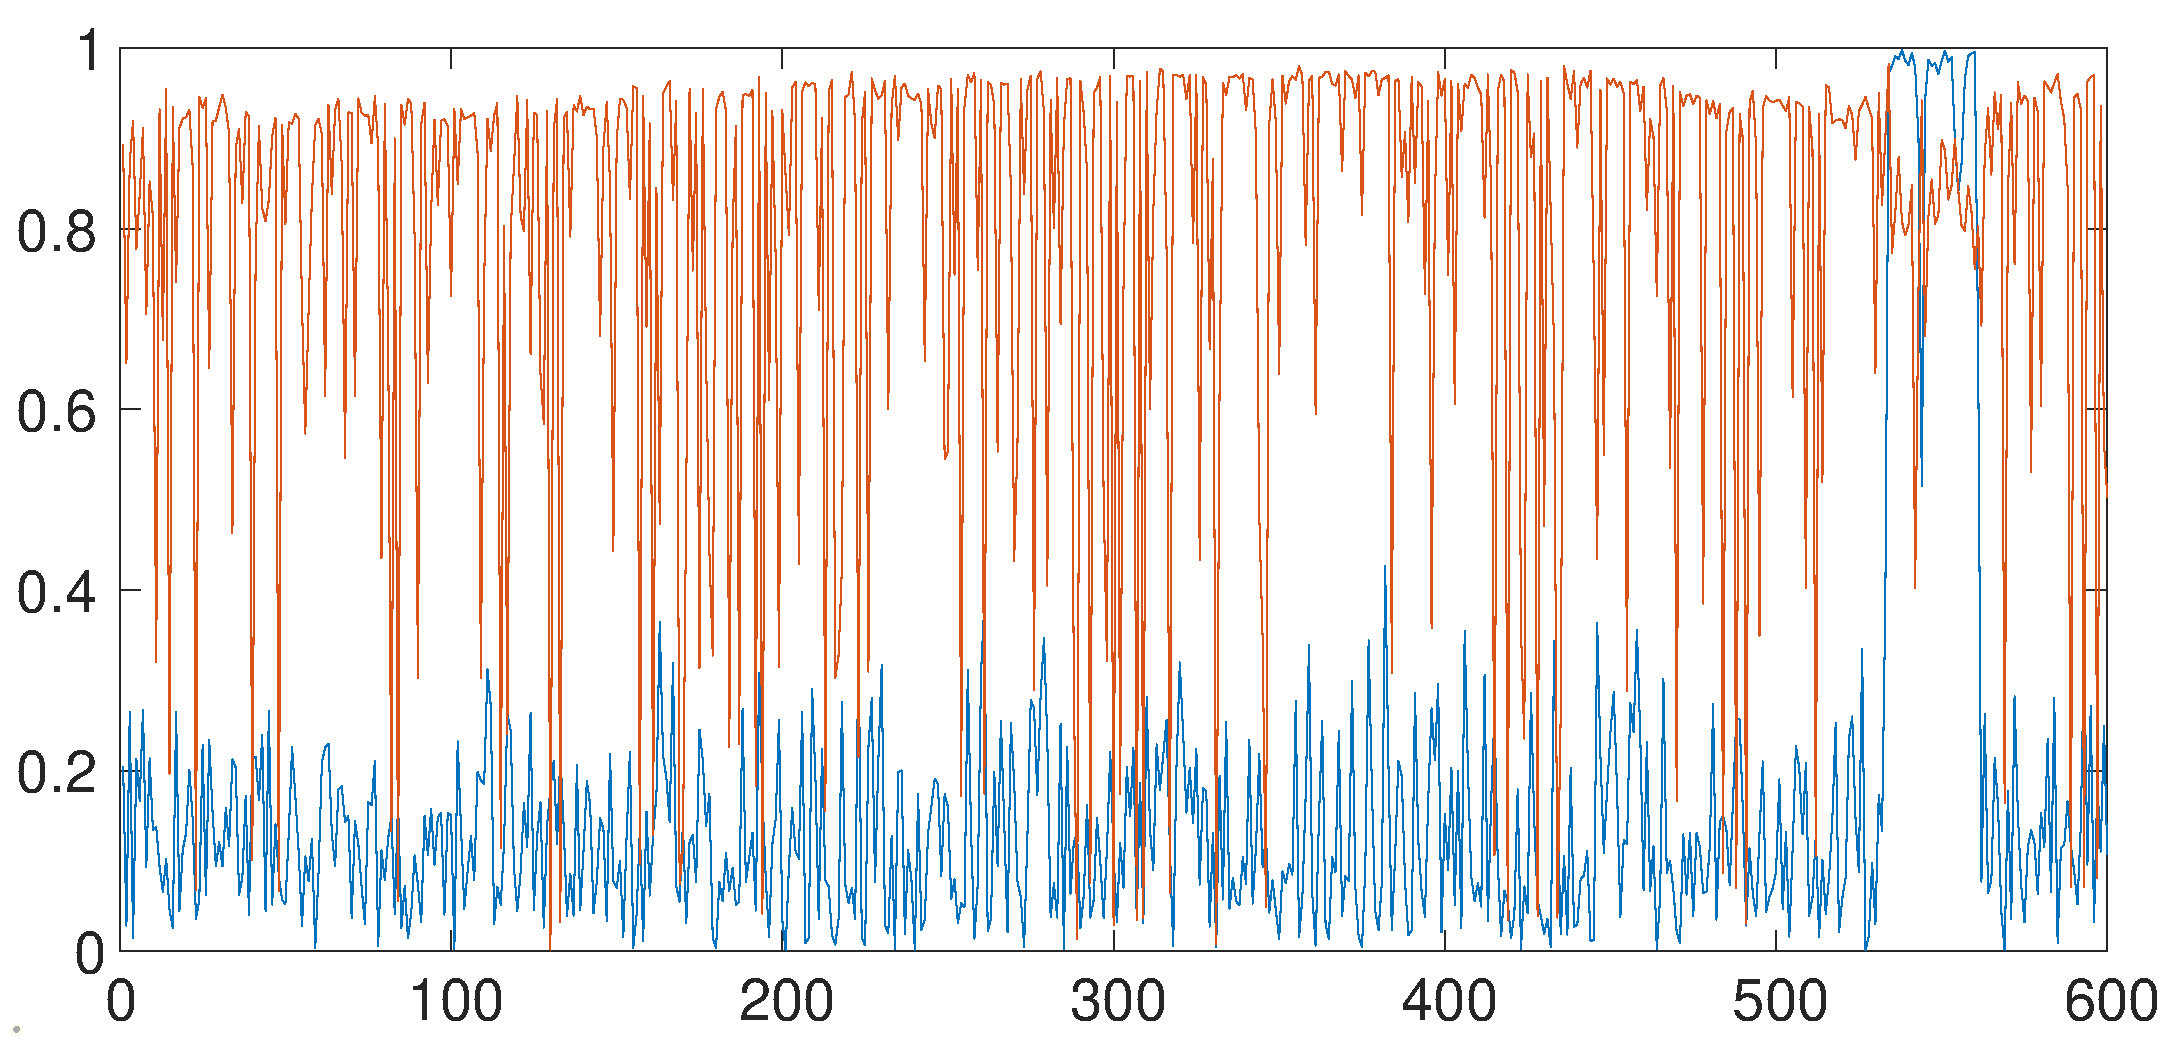
\includegraphics[width=0.3\textwidth]{images/fdd-xcorr/indoor-no-move.eps}
    }
    \subfigure[室内-方式2]{
        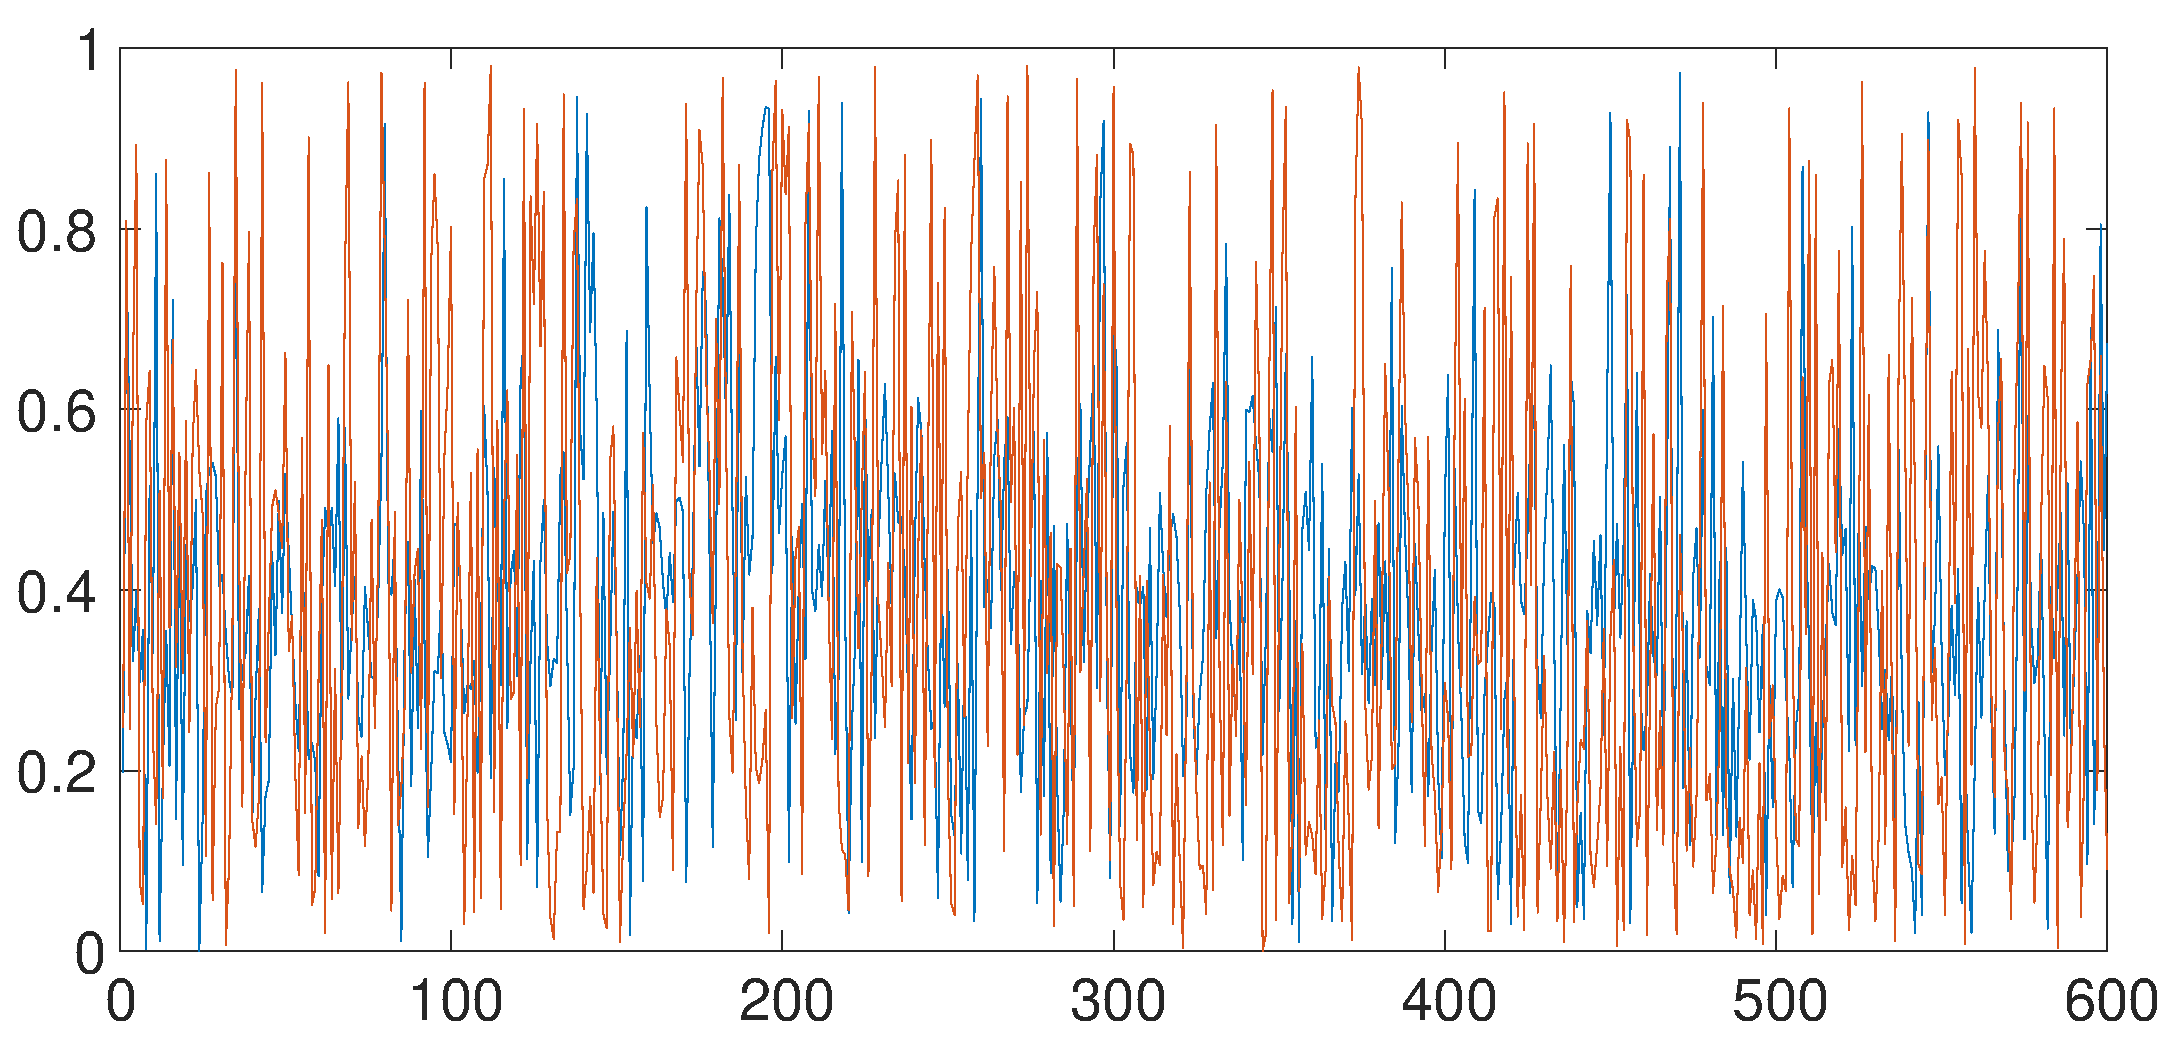
\includegraphics[width=0.3\textwidth]{images/fdd-xcorr/indoor-people-move.eps}
    }
    \subfigure[室内-方式3]{
        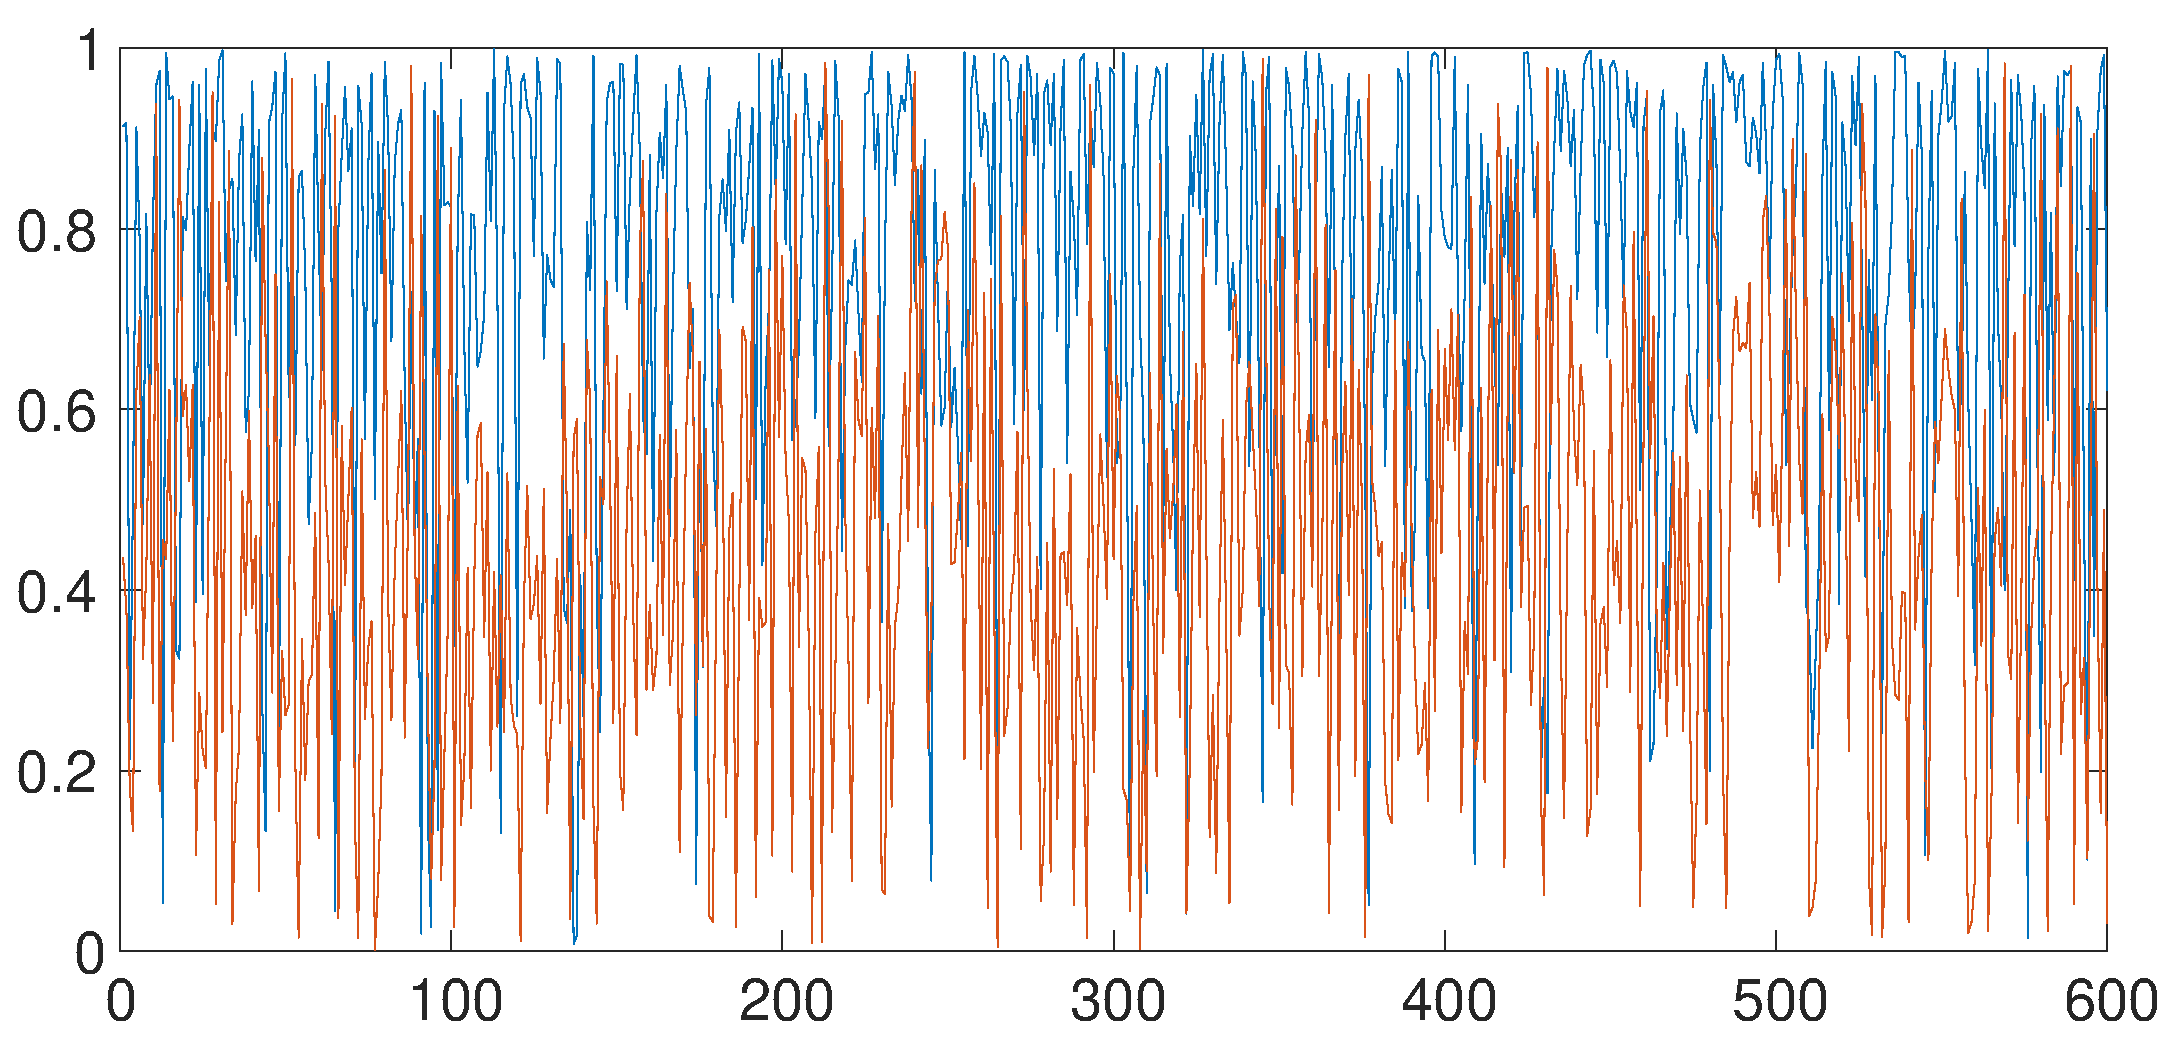
\includegraphics[width=0.3\textwidth]{images/fdd-xcorr/indoor-trolly-move.eps}
    }
    \quad    %用 \quad 来换行
    \subfigure[走廊-方式1]{
        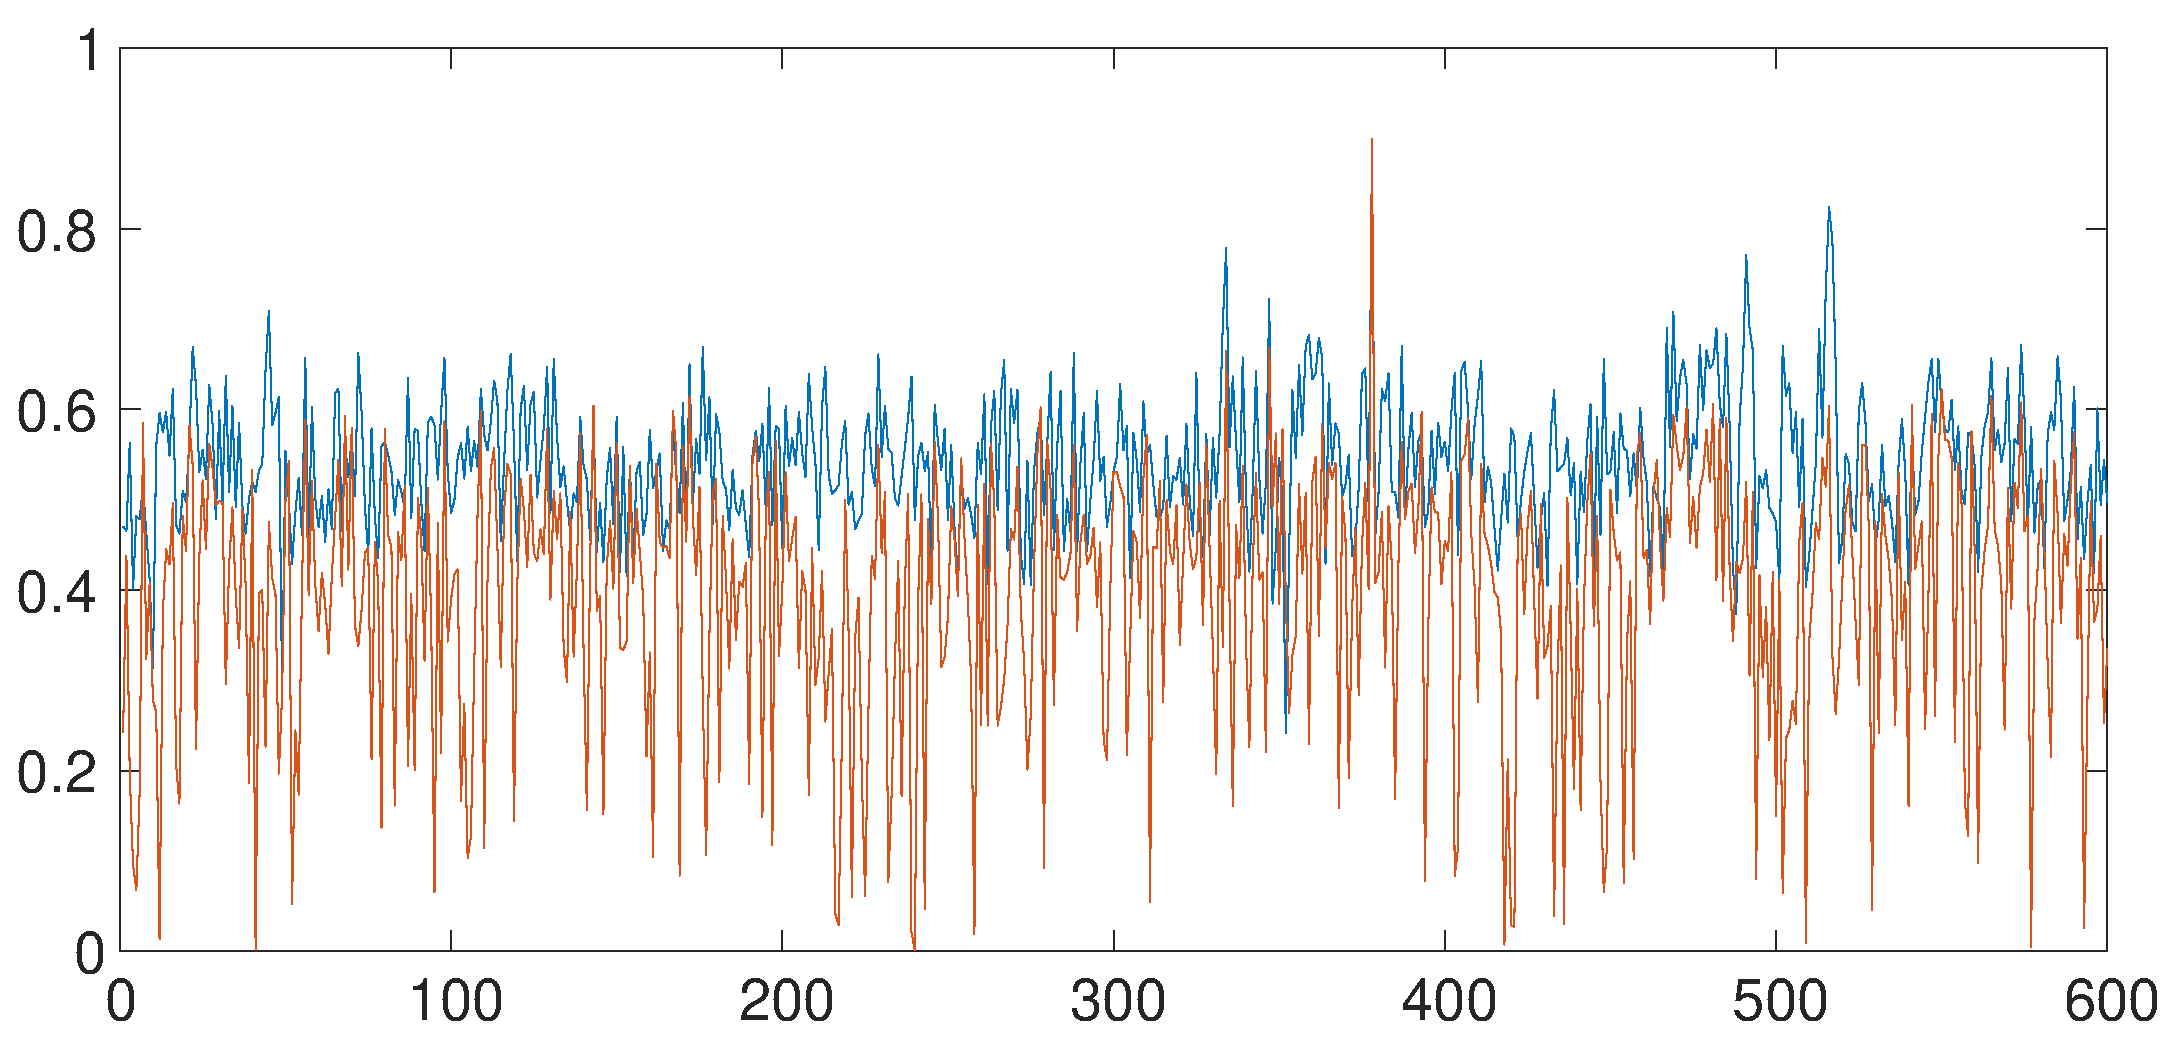
\includegraphics[width=0.3\textwidth]{images/fdd-xcorr/corridor-no-move.eps}
    }
    \subfigure[走廊-方式2]{
        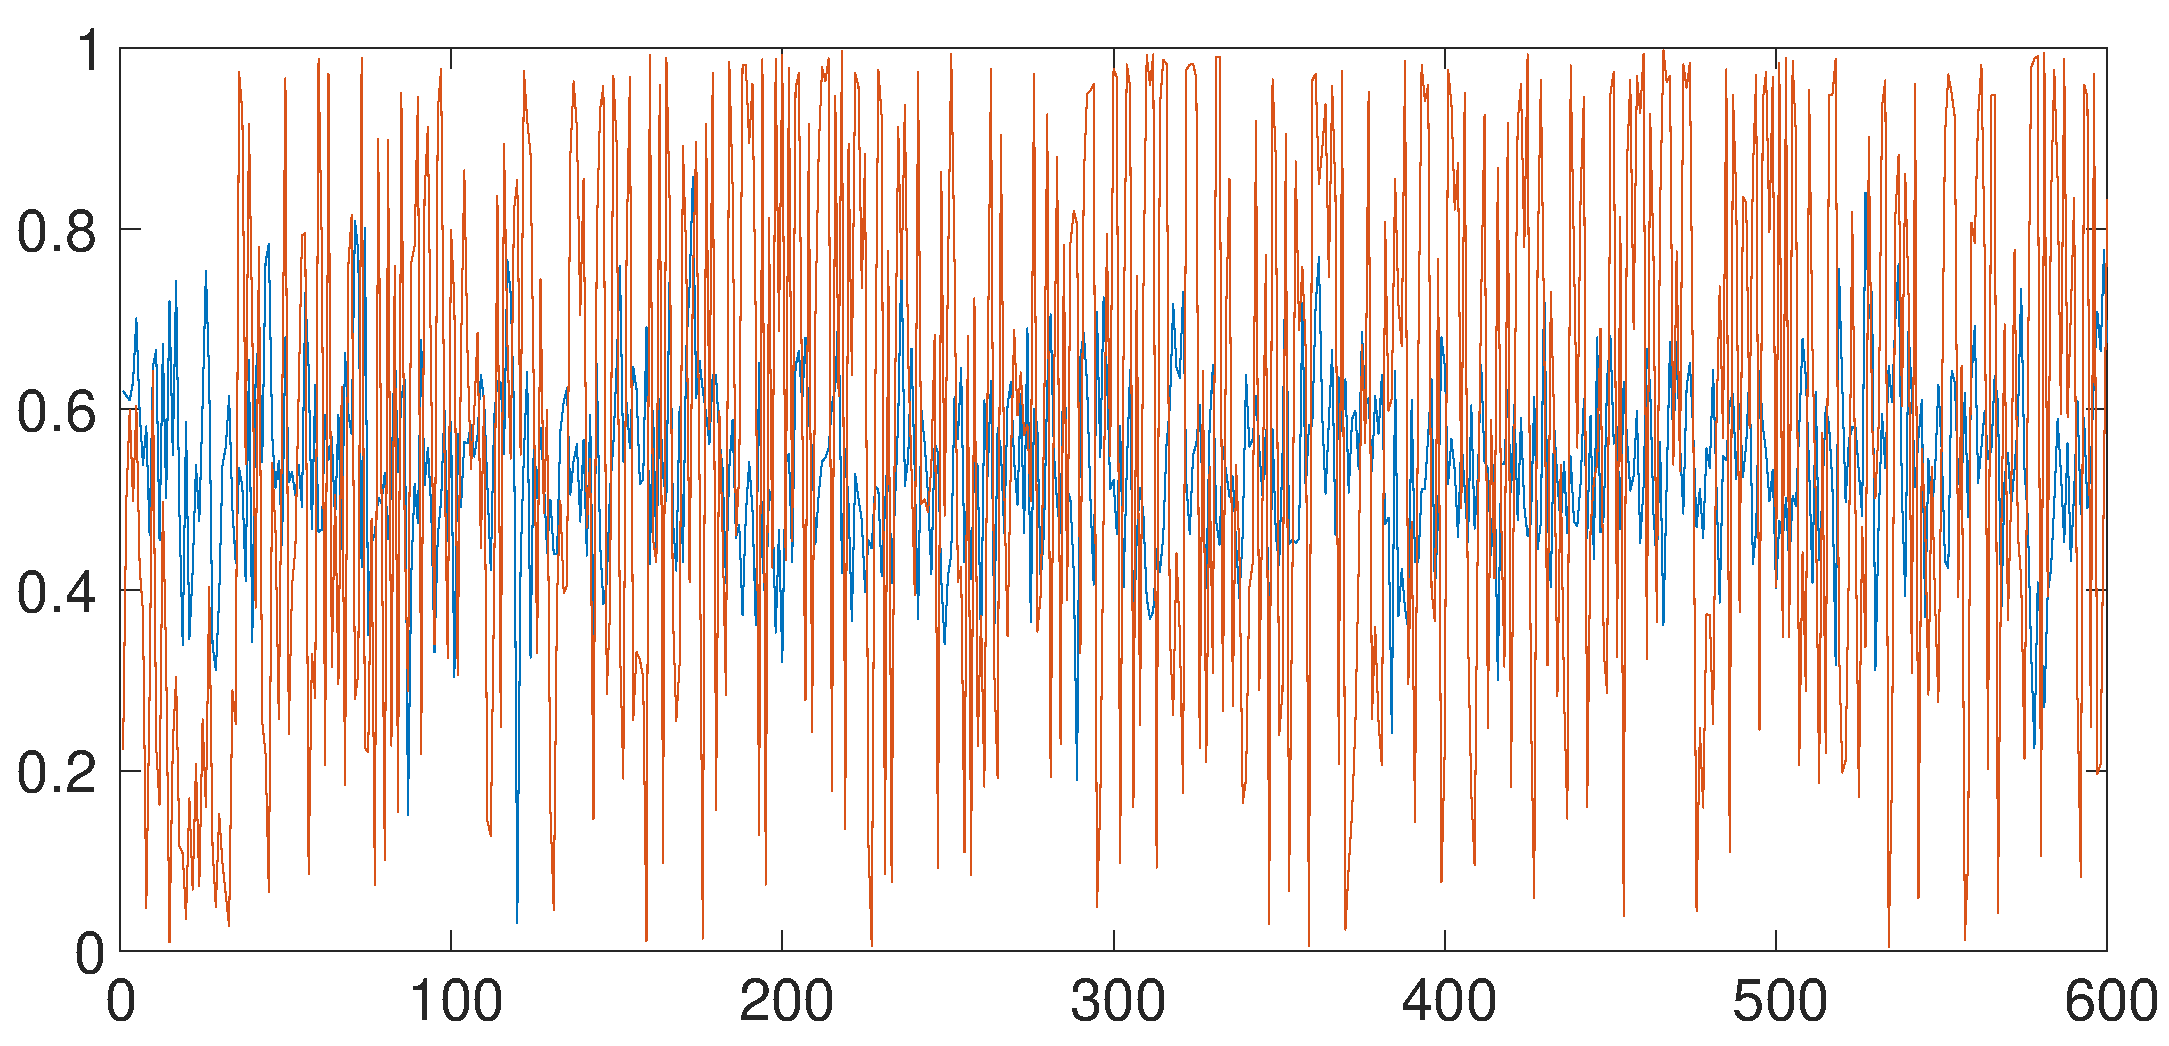
\includegraphics[width=0.3\textwidth]{images/fdd-xcorr/corridor-people-move.eps}
    }
    \subfigure[走廊-方式3]{
        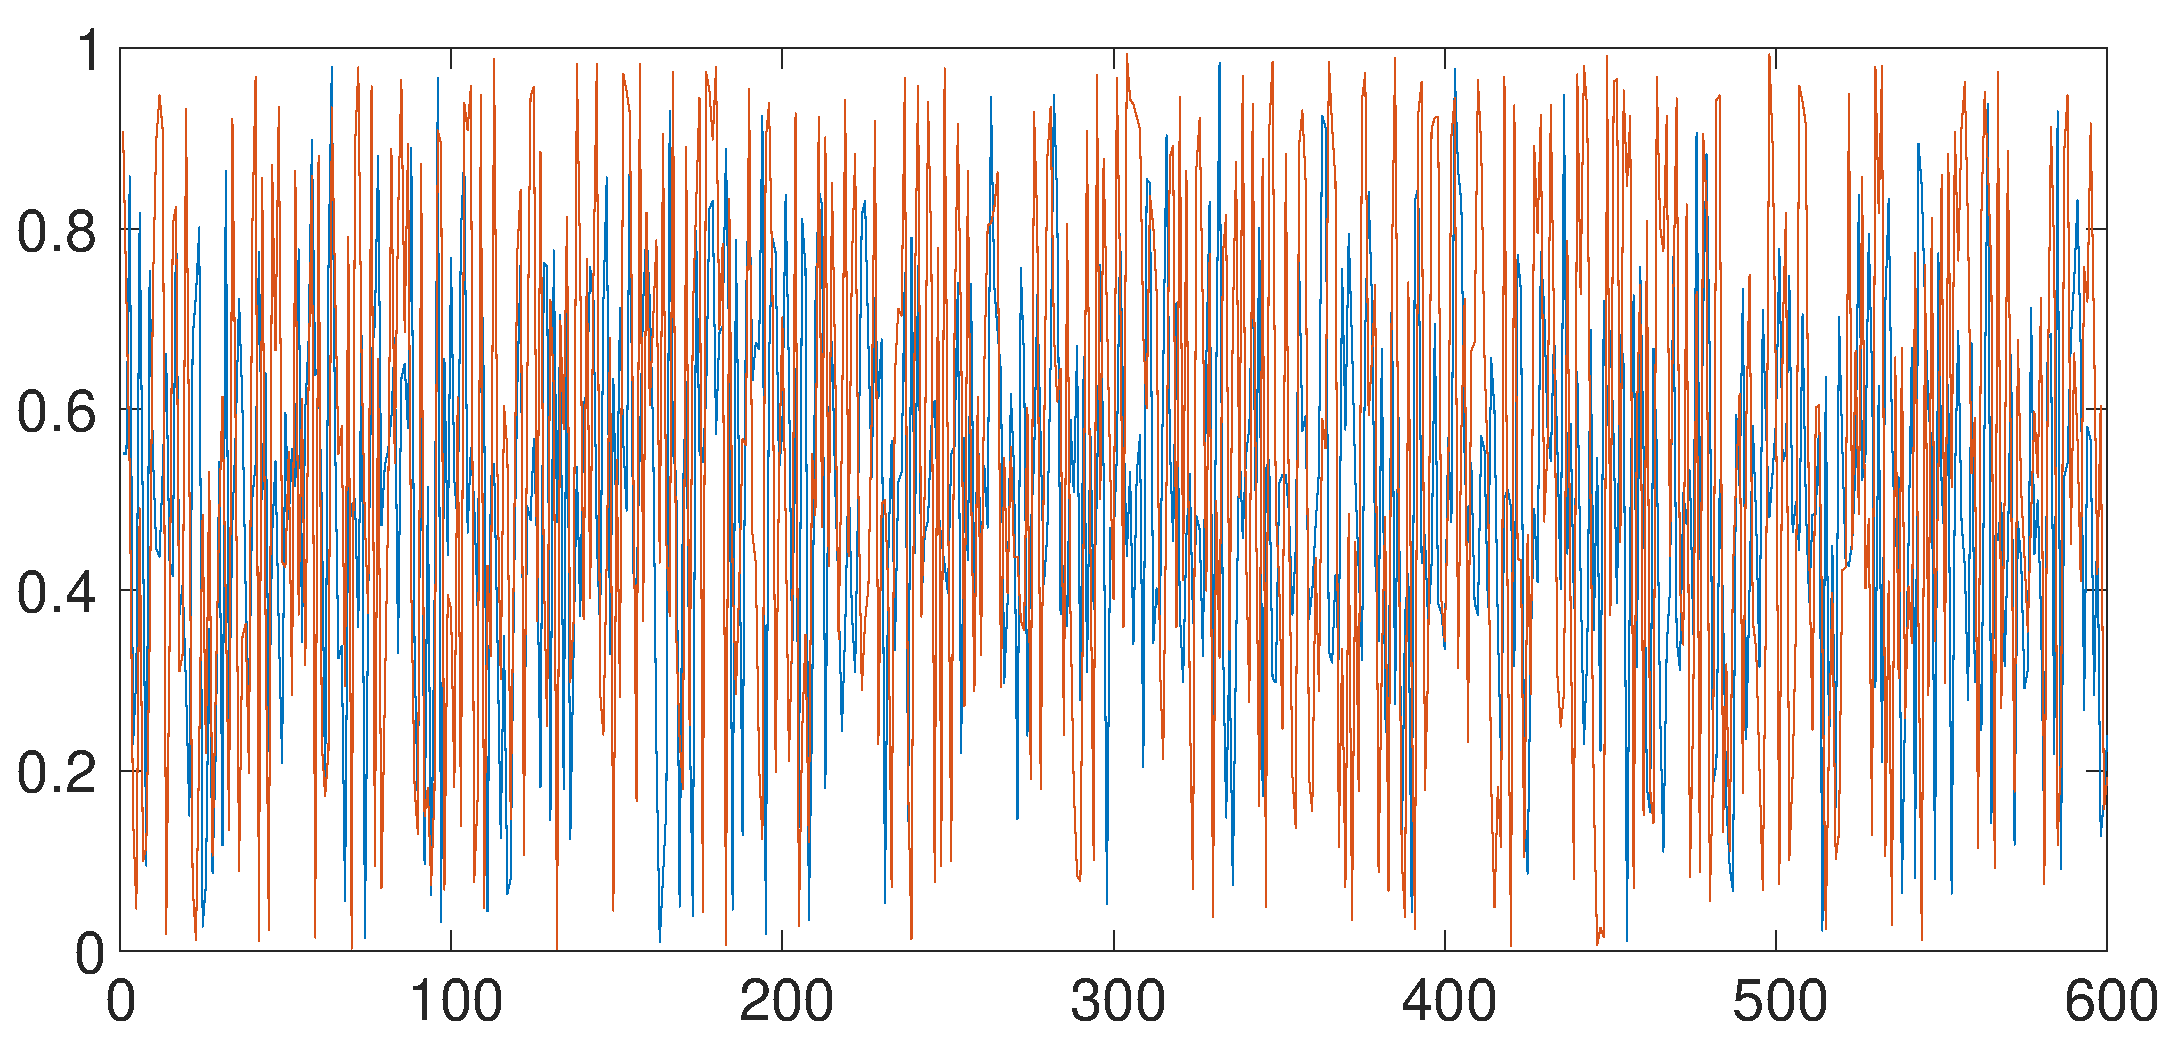
\includegraphics[width=0.3\textwidth]{images/fdd-xcorr/corridor-trolly-move.eps}
    }
    \quad
    \subfigure[室外-方式1]{
        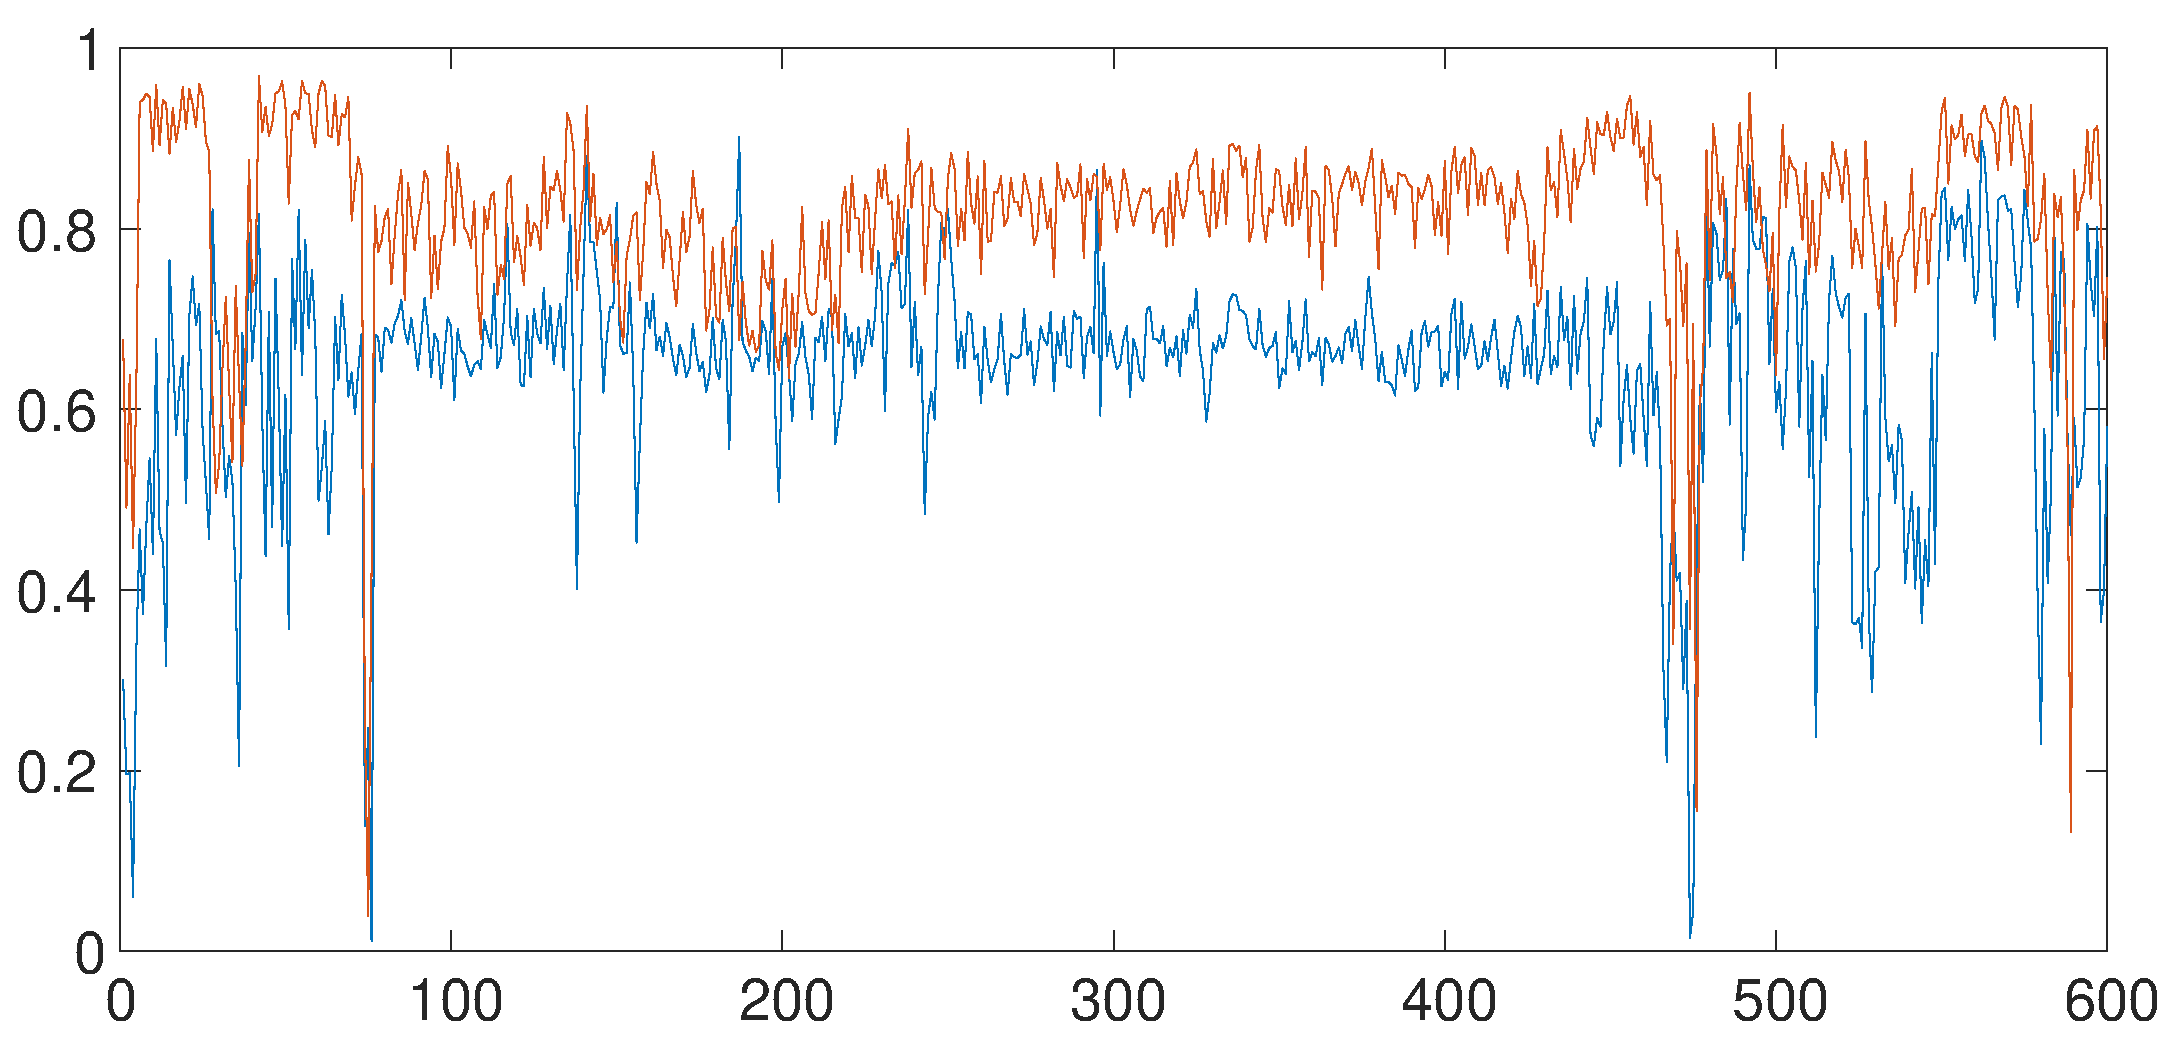
\includegraphics[width=0.3\textwidth]{images/fdd-xcorr/outdoor-no-move.eps}
    }
    \subfigure[室外-方式2]{
        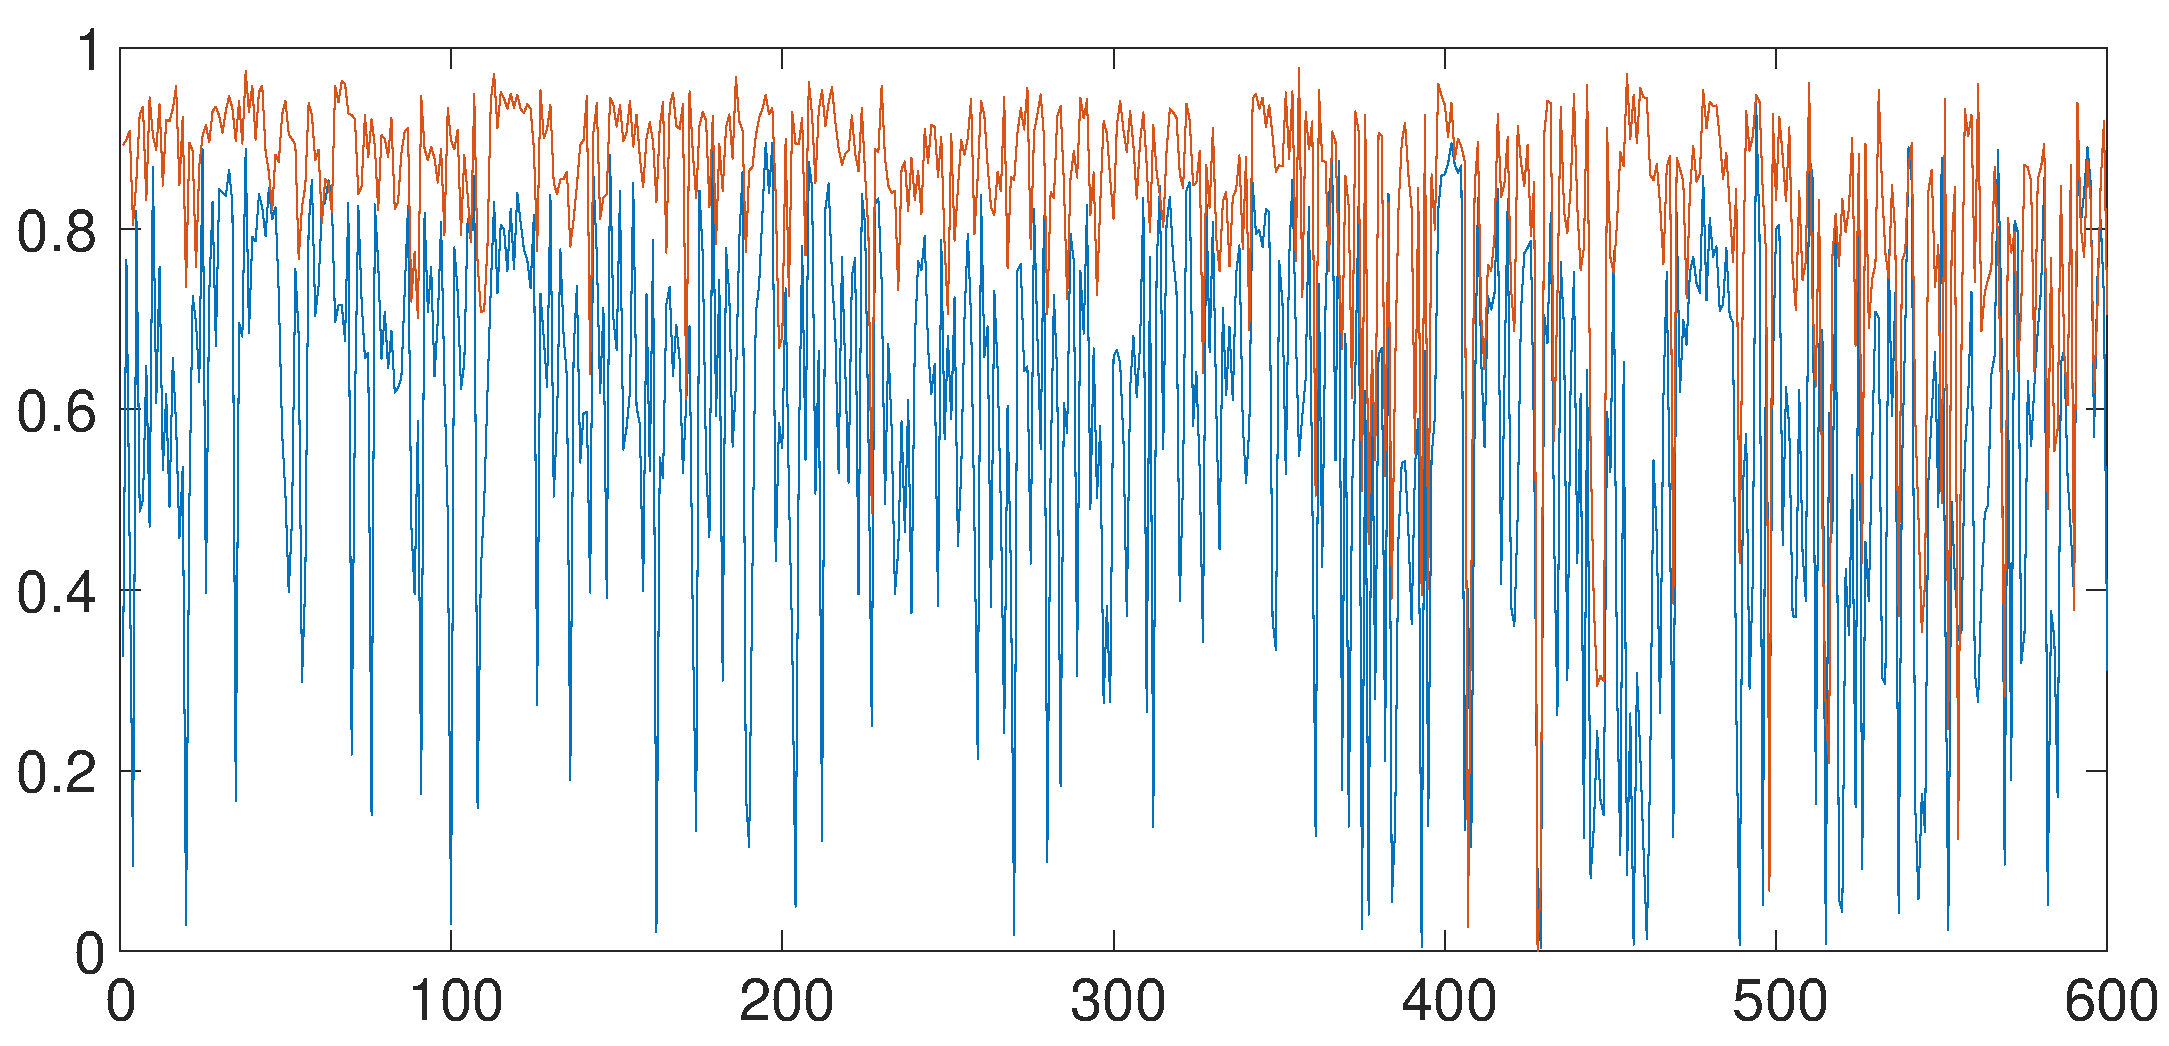
\includegraphics[width=0.3\textwidth]{images/fdd-xcorr/outdoor-people-move.eps}
    }
    \subfigure[室外-方式3]{
        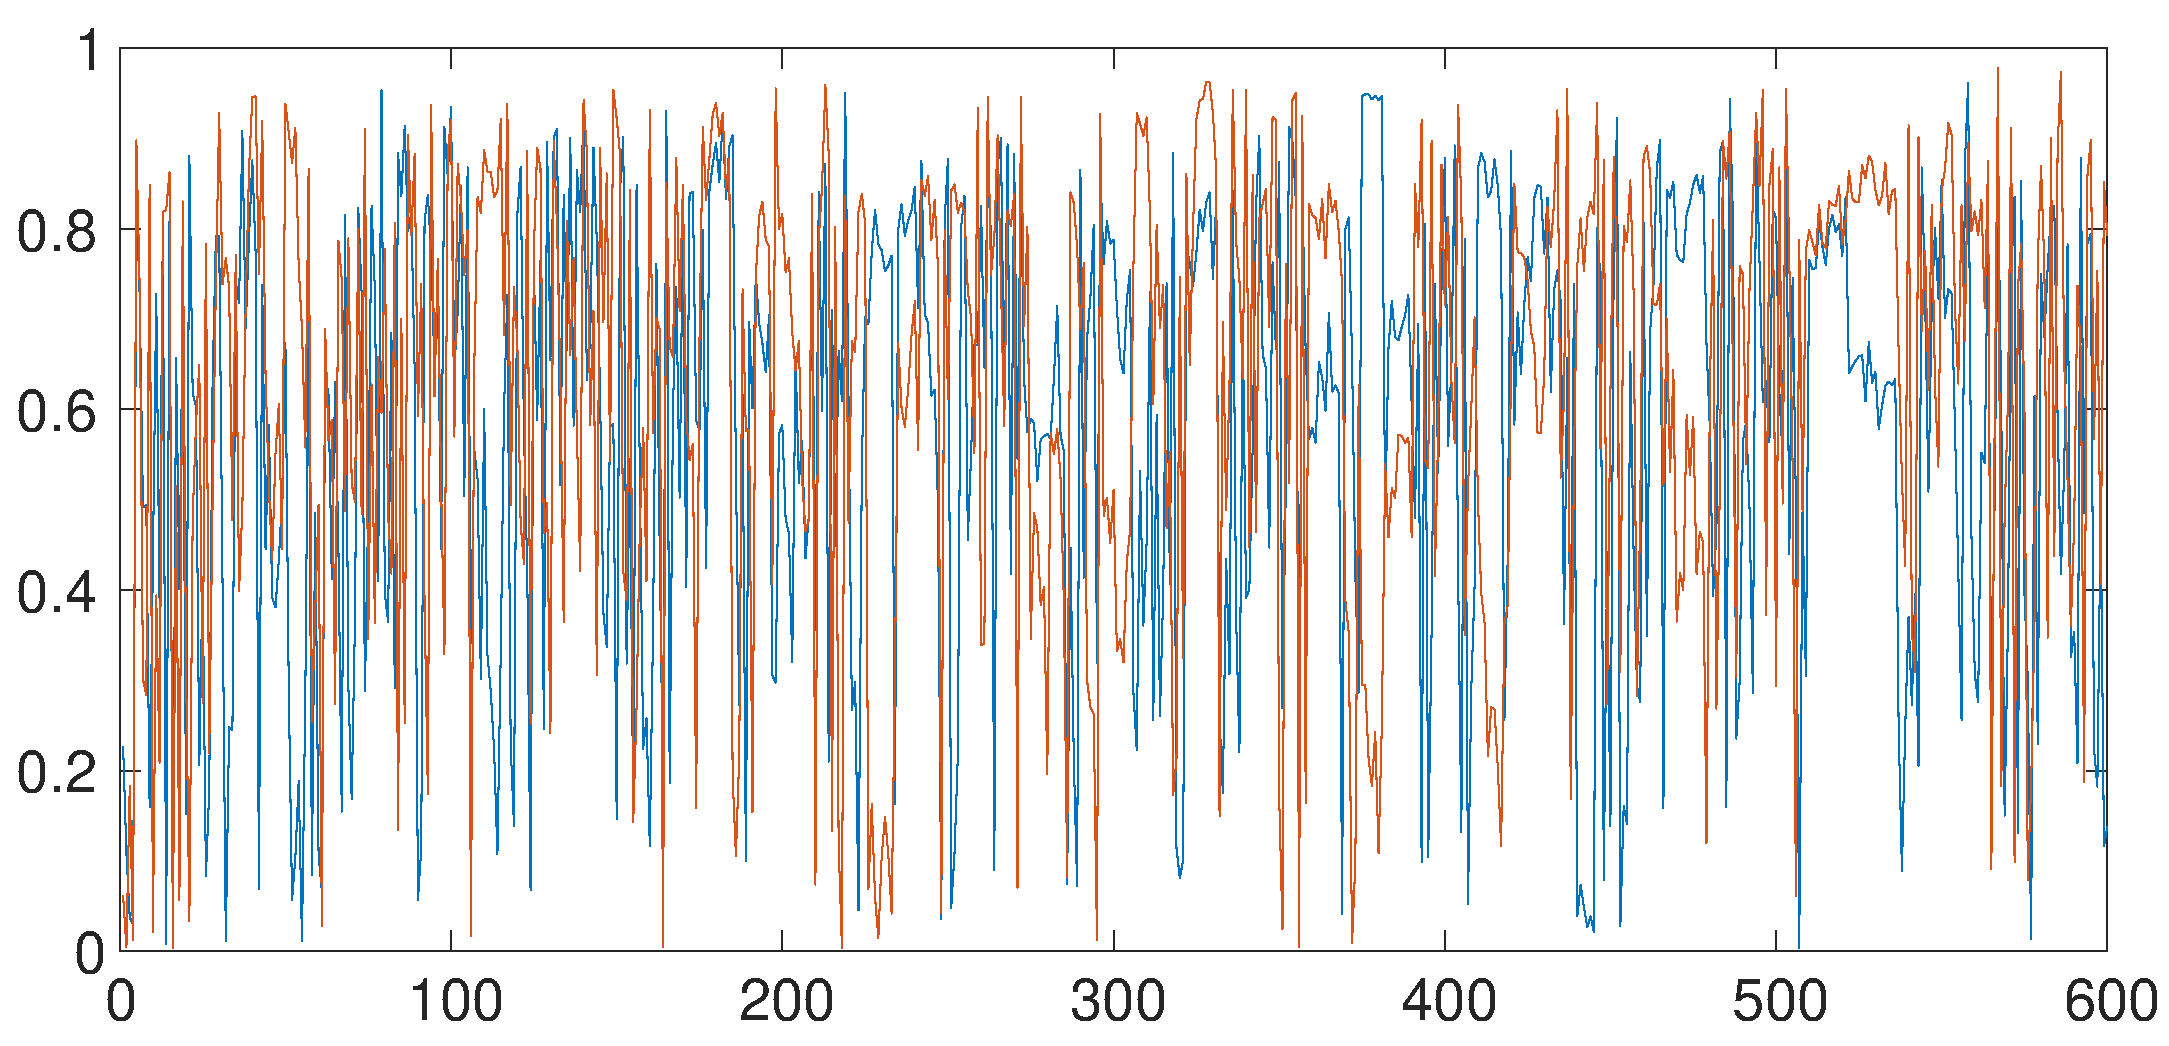
\includegraphics[width=0.3\textwidth]{images/fdd-xcorr/outdoor-trolly-move.eps}
    }
    \caption{不同场景与环境下Alice和Bob、Alice和Eve之间CSI相关系数}{} % xcorr between alice and bob, xcorr between bob and eve
    \label{fdd_csi_xcorr}
\end{figure}

将多组数据取平均,得到9种情况下,Alice、Bob和Eve之间的平均皮尔逊相关系数如图\ref{tdd_bar_xcorr}所示。在9种情况下,Alice与Bob之间互相关系数最高为0.7569,该情况出现在室内房间终端的情况。而Alice与Eve之间互相关系数最高为0.8303,该情况出现在空旷室外人员走动的场景。之所以出现Alice与Bob之间互相关系数低于Alice与Eve之间互相关系数,是因为频率选择性对信道互易性的影响,Alice和Bob在FDD模式下的互易性较差。FDD模式下的信道互易性与各个场景、终端是否移动、人员是否移动无明显关系,这是由于上下行载波频率不同,载波频率的差值对信道互易性更大。

% todo 等到实验室,用大屏把图重新绘制一下。
\begin{figure}[htbp!]
    \centering \includegraphics[width=0.9\textwidth]{images/fdd-xcorr/bar2.eps}
    \caption{不同场景下三者之间的互相关系数柱状图}
    \label{fdd_bar_xcorr}
\end{figure}

\subsection{信息泄漏率}

和TDD一样,本文在9种情况下按照公式(\ref{safe_rate_equation})计算了多组安全信息率并取平均,9种情况下的平均安全信息率如图\ref{fdd_bar_leak}所示。

分析图中结果可知,无论是室内、走廊还是室外,均是当终端移动时安全信息率最高,其中在室内终端移动时,信息安全比率高达67.74\%,这也是所有情况中的最高值,在室外终端移动时,信息安全比率为41.49\%。在所有情况中,室外终端固定时的信息安全比率最低,低至15.57\%。9种情况的平均安全信息率具体数据为表\ref{fdd_bar_leak_data}。


\begin{figure}[htbp!]
    \centering \includegraphics[width=0.9\textwidth]{images/fdd-leak/bar.eps}
    \caption{不同场景下的平均安全信息率柱状图}
    \label{fdd_bar_leak}
\end{figure}

\begin{table}[htbp] % 依赖包 booktabs
    \centering
    \setlength{\tabcolsep}{16mm}{
    \begin{tabular}{cccc}
    \toprule
        & \textbf{方式1} & \textbf{方式2} & \textbf{方式3} \\
    \midrule
    室内 & 0.3379 & 0.5654 & 0.6774 \\ 
	走廊 & 0.3925 & 0.4075 & 0.4703 \\ 
    室外 & 0.1557 & 0.2231 & 0.4149 \\
    \bottomrule
    \end{tabular}
    }
    \caption{不同场景下的平均安全信息率数值
    \label{fdd_bar_leak_data}}
\end{table}


本文计算出室内、走廊、室外三种场景下,所有信道环境下的安全信息率平均值,如表\ref{fdd_three_scene_avg}所示。表中结果说明各种信道环境下,室内的信息安全比率最高,高达52.69\%,室外的信息安全比率最低,低至26.46\%。也计算出终端固定、人员移动、终端移动三种信道环境下,所有场景的安全信息率平均值,如表\ref{fdd_three_channel_env_avg}。表中说,各种场景下,终端移动的安全比率最高,高达52.09\%,终端固定的安全比率最低,低至29.54\%。从结果中可以看出,适当的多普勒效应可以提高FDD模式下无线密钥生成系统的信息安全比率。相对于终端固定和人员走动的信道环境,终端移动的信道环境可以提高系统的信息安全比率。和TDD不同的是,相对于走廊和室外,室内房间和走廊场景会提高信息安全比率。

\begin{table}[]
    \centering
    \setlength{\tabcolsep}{22mm}{
    \begin{tabular}{ccc}
    \toprule
    室内 & 走廊 & 室外 \\ 
    \midrule
    52.69\% & 42.34\% & 26.46\% \\ 
    \bottomrule
    \end{tabular}
    }
    \caption{室内、走廊和室外三种场景的平均安全信息率
    \label{fdd_three_scene_avg}}
\end{table}

\begin{table}[]
    \centering
    \setlength{\tabcolsep}{20mm}{
    \begin{tabular}{ccc}
    \toprule
    终端固定 & 人员移动 & 终端移动 \\
    \midrule
    29.54\% & 39.86\% & 52.09\% \\ 
    \bottomrule
    \end{tabular}
    }
    \caption{终端固定、人员走动和终端移动三种信道环境的平均安全信息率
    \label{fdd_three_channel_env_avg}}
\end{table}

\subsection{随机性评估}

与TDD相同,本文使用频域的图像熵以及NIST随机性测试分别评估CSI随机性和密钥随机性。

\subsubsection{CSI随机性}

本文在上一章中已经计算了信道无多径且不随时间变化、信道有多径且不随时间变化、信道随时间不同完全随机变化三种特殊情况下的CSI作为对比,其CSI以及熵值如图\ref{special_csi}和\ref{entropy_spectial}。因此本文FDD模式下计算出的CSI图像熵也应该出现在0.00006~7.0098之间。

本文在每个情况下,使用600组CSI按照公式(\ref{entropy_fft2d_equation})计算多组CSI的图像熵,如表\ref{fdd_entropy_fft2d}。从表中可以看出,无论哪种场景,终端固定的信道环境下的CSI随机性最低,终端移动的信道环境下的CSI随机性最高,这一点与TDD模式相同。与TDD相反的是,无论哪种信道环境,室内场景的CSI随机性最高,室外场景的CSI随机性最低。所有情况中,在室外场景下的终端固定时CSI随机性最低,低至1.7776;在室内场景下的终端移动时CSI随机性最高,高达4.8971。从表中分析得知,随着信道环境更加复杂,系统探测的CSI随机性也会增加。但是,室内场景测量的CSI随机性更好于室外场景测量。

\begin{table}[]
    \centering
    \setlength{\tabcolsep}{16mm}{
    \begin{tabular}{cccc} 
        \toprule
        & \textbf{方式1} & \textbf{方式2} & \textbf{方式3} \\
        \midrule
        室内 & 3.9730 & 4.5164 & 4.8971 \\ 
        走廊 & 3.1899 & 3.1137 & 3.1377 \\ 
        室外 & 1.7776 & 2.1263 & 2.6909 \\
        \bottomrule
    \end{tabular}
    }
    \caption{不同场景的图像熵值
    \label{fdd_entropy_fft2d}}
\end{table}


\subsubsection{密钥随机性}

同TDD一样,本文选择本文选择NIST随机性测试中的7种随机性测试,分别计算了降采样率为1、4、8时的测试结果,分别如表\ref{fdd_NIST_test_result_1}、\ref{fdd_NIST_test_result_4}、\ref{fdd_NIST_test_result_8}所示。图中数据为,600组数据中,通过NIST测试的比例,在图中标记出比例小于1\%的数据。从图中可以看出,随着降采样率提高,比率小于1\%的数据减少,密钥随机性提高。在降采样率为1时,系统生成的密钥数据在游程检验、块内最长最长游程检验序列检验、近似熵检验等多项测试表现极差。在降采样率为4时,密钥数据主要在块内频数检验、块内最长游程检验的测试中表现较差。在降采样率为8时,密钥数据主要在块内最长游程检验表现较差。观察比率小于1\%的数据分布可知,走廊和室外场景下的密钥数据在随机性测试中表现良好,而室内密钥数据未通过测试的比率极大。同TDD模式比较可知,TDD模式下生成密钥数据随机性更好,通过测试比率更高。


\begin{table}[]
    \centering
    \tabulinesep=1.2mm
    \begin{tabu}to \linewidth{X[c,m]X[c,m]X[c,m]X[c,m]X[c,m]X[c,m]X[c,m]X[c,m]X[c,m]X[c,m]}
        \toprule
        \textbf{} & \textbf{室内-方式1} & \textbf{室内-方式2} & \textbf{室内-方式3} & \textbf{走廊-方式1} & \textbf{走廊-方式2} & \textbf{走廊-方式3} & 
        \textbf{室外-方式1} & \textbf{室外-方式2} & \textbf{室外-方式3} \\
        \midrule

        频率检验 & \underline{02.83\%}    & 04.50\%    & 07.83\%    & 01.00\%    & 04.67\%    & 15.50\%    & 85.33\%    & 43.67\%    & 26.33\% \\
        块内频数检验 & 96.00\%    & 98.67\%    & 72.33\%    & 99.83\%    & 98.00\%    & 87.50\%    & 96.17\%    & 81.50\%    & 67.83\% \\
        游程检验 & \underline{00.50\%}    & \underline{00.17\%}    & \underline{00.50\%}    & \underline{00.17\%}    & 01.50\%    & 05.00\%    & 01.00\%    & 04.33\%    & 05.33\% \\
        块内最长游程检验 & \underline{00.00\%}    & \underline{00.00\%}    & \underline{00.17\%}    & \underline{00.00\%}    & 01.17\%    & 01.83\%    & 01.67\%    & 01.83\%    & 04.17\% \\
        % 二元矩阵秩检验 & 52.83\%    & 62.33\%    & 57.50\%    & 29.00\%    & 29.50\%    & 50.83\%    & 50.67\%    & 45.67\%    & 41.33\% \\
        序列检验 & \underline{00.50\%}    & \underline{00.17\%}    & \underline{00.50\%}    & \underline{00.17\%}    & 01.50\%    & 03.50\%    & 01.00\%    & 03.00\%    & 02.67\% \\
        近似熵检验 & \underline{00.33\%}    & \underline{00.17\%}    & \underline{00.67\%}    & \underline{00.17\%}    & 01.83\%    & 03.83\%    & 01.00\%    & 03.17\%    & 02.33\% \\
        累加和检验 & 96.50\%    & 97.17\%    & 75.50\%    & 99.67\%    & 96.33\%    & 92.33\%    & 96.00\%    & 84.83\%    & 83.00\% \\
        \bottomrule
    \end{tabu}
    \caption{NIST测试结果 降采样数为1
    \label{fdd_NIST_test_result_1}}
\end{table}

\begin{table}[]
    \centering
    \tabulinesep=1.2mm        
    \begin{tabu}to \linewidth{X[c,m]X[c,m]X[c,m]X[c,m]X[c,m]X[c,m]X[c,m]X[c,m]X[c,m]X[c,m]}
        \toprule
        \textbf{} & \textbf{室内-方式1} & \textbf{室内-方式2} & \textbf{室内-方式3} & \textbf{走廊-方式1} & \textbf{走廊-方式2} & \textbf{走廊-方式3} & 
        \textbf{室外-方式1} & \textbf{室外-方式2} & \textbf{室外-方式3} \\
        \midrule

        频率检验 & 61.83\%    & 20.33\%    & 26.50\%    & 02.33\%    & 11.67\%    & 39.00\%    & 95.67\%    & 78.00\%    & 61.83\% \\
        块内频数检验 & \underline{00.00\%}    & \underline{00.00\%}    & 99.50\%    & \underline{00.00\%}    & \underline{00.00\%}    & 99.33\%    & \underline{00.00\%}    & 99.50\%    & 99.33\% \\
        游程检验 & 02.33\%    & 02.00\%    & 05.50\%    & 00.33\%    & 05.50\%    & 22.67\%    & 23.00\%    & 38.33\%    & 46.67\% \\
        块内最长游程检验 & \underline{00.00\%}    & \underline{00.17\%}    & 01.17\%    & \underline{00.00\%}    & \underline{00.17\%}    & 01.83\%    & 05.00\%    & 09.50\%    & 11.17\% \\
        % 二元矩阵秩检验 & 04.83\%    & 02.17\%    & 36.33\%    & \underline{00.00\%}    & \underline{00.17\%}    & \underline{00.83\%}    & \underline{00.00\%}    & \underline{00.00\%}    & \underline{00.67\%} \\
        序列检验 & 24.83\%    & 05.33\%    & 08.33\%    & \underline{00.50\%}    & 04.83\%    & 19.00\%    & 22.00\%    & 37.33\%    & 37.83\% \\
        近似熵检验 & 03.00\%    & 02.83\%    & 05.33\%    & \underline{00.50\%}    & 03.67\%    & 18.50\%    & 39.17\%    & 39.83\%    & 39.33\% \\
        累加和检验 & 99.83\%    & \underline{00.00\%}    & 92.50\%    & \underline{00.00\%}    & 99.17\%    & 97.67\%    & 99.83\%    & 98.50\%    & 97.00\% \\
        
        \bottomrule
    \end{tabu}
    \caption{NIST测试结果 降采样数为4
    \label{fdd_NIST_test_result_4}}
\end{table}


\begin{table}[]
    \centering
    % \setlength{\tabcolsep}{0.2mm}{
    \tabulinesep=1.2mm        
    \begin{tabu} to \linewidth{X[c,m]X[c,m]X[c,m]X[c,m]X[c,m]X[c,m]X[c,m]X[c,m]X[c,m]X[c,m]}
        \toprule
        \textbf{} & \textbf{室内-方式1} & \textbf{室内-方式2} & \textbf{室内-方式3} & \textbf{走廊-方式1} & \textbf{走廊-方式2} & \textbf{走廊-方式3} & 
        \textbf{室外-方式1} & \textbf{室外-方式2} & \textbf{室外-方式3} \\
        \midrule

        频率检验 & 97.17\%    & 68.00\%    & 59.67\%    & 44.00\%    & 47.83\%    & 74.00\%    & 96.17\%    & 88.33\%    & 79.33\% \\
        块内频数检验 & \underline{00.00\%}    & \underline{00.00\%}    & 99.50\%    & \underline{00.00\%}    & 99.17\%    & 97.83\%    & 97.33\%    & 96.50\%    & 95.17\% \\
        游程检验 & 49.67\%    & 13.00\%    & 15.50\%    & \underline{00.83\%}    & 07.17\%    & 36.83\%    & 82.50\%    & 75.00\%    & 71.50\% \\
        块内最长游程检验 & \underline{00.00\%}    & \underline{00.17\%}    & \underline{00.33\%}    & \underline{00.00\%}    & \underline{00.00\%}    & \underline{00.00\%}    & \underline{00.00\%}    & \underline{00.00\%}    & \underline{00.00\%} \\
        % 二元矩阵秩检验 & \underline{00.00\%}    & \underline{00.00\%}    & \underline{00.00\%}    & \underline{00.00\%}    & underline{00.00\%}    & \underline{00.00\%}    & \underline{00.00\%}    & \underline{00.00\%}    & \underline{00.00\%} \\
        序列检验 & 91.17\%    & 36.17\%    & 18.50\%    & 05.33\%    & 13.83\%    & 40.33\%    & 76.83\%    & 62.67\%    & 50.83\% \\
        近似熵检验 & 21.50\%    & 09.83\%    & 13.83\%    & 01.00\%    & 06.67\%    & 30.33\%    & 89.33\%    & 67.33\%    & 56.33\% \\
        累加和检验 & \underline{00.00\%}    & \underline{00.00\%}    & 99.33\%    & \underline{00.00\%}    & 99.00\%    & 96.50\%    & 97.33\%    & 95.83\%    & 94.17\% \\
       
        \bottomrule
    \end{tabu}
    % }
    \caption{NIST测试结果 降采样数为8
    \label{fdd_NIST_test_result_8}}
\end{table}

\subsection{密钥生成速率}

同TDD一样,密钥生成速率与采样率成反比。本文计算了室内终端固定情况下,FDD模式下不同降采样率的密钥生成速率,如图\ref{fdd-keyrate}所示。观察可知,密钥生成速率随着降采样率升高而降低。在采样率
为 4 时,密钥生成速率高达 28.6667 bits/s,在采样率为 20 时,密钥生成速率降低到 4.6667 bits/s。显然,FDD模式下密钥生成速率低于TDD模式,这是因为FDD模式下信道互易性较差,所以导致通过CRC检验的组数较小,因此FDD模式下密钥生成率较低。


\begin{figure}[htbp!]
    \centering \includegraphics[width=0.9\textwidth]{images/fdd-keyrate.eps}
    \caption{不同降采样率的密钥生成速率}
    \label{fdd-keyrate}
\end{figure}


\subsection{纠错码对密钥一致率}

本文使用FDD模式下实测数据,分析FDD模式下纠错码的纠错性能。同TDD模式一样,本文分别计算9种情况下BCH码和Turbo码的纠错能力,每种情况使用600组数据计算平均密钥一致率及其对应的平均误码率。如图\ref{bar-bch-ber-nine}为9种情况下BCH码的纠错效果,其中参数N = 31, K = 11。具体数据见表格\ref{fdd-bch-ber-nine},


表中结果表明,误比特率和密钥一致率成反比。所有场景中,密钥一致率最高为室内终端移动的77.05\%,其也对应着最低的误比特率24.07\%;密钥一致率最低为室内终端固定情况下的60.92\%,其也对应着最高的误比特率39.38\%。

如图\ref{fdd-bar-turbo-ber-nine}为9种情况下Turbo码的纠错效果,其中迭代次数为8,N = 2, K = 3,生成多项式为g = [1 1 1; 1 0 1]。所有场景中,密钥一致率最高为室内终端移动的77.05\%,其也对应着最低的误比特率22.89\%;密钥一致率最低为室内终端固定情况下的60.92\%,其对应这最高的误比特率42.54\%。根据表中结果,Turbo纠错性能好于BCH码。此外,无论是BCH码还是Turbo码,相对于TDD模式的系统纠错性能,FDD模式下纠错性能均差于TDD模式,这是因为FDD模式下密钥一致率较低。

\begin{figure}[htbp!]
    \centering \includegraphics[width=0.9\textwidth]{images/fdd-encode/bch-ber-nine.eps}
    \caption{不同情况下BCH的平均误码率以及对应的平均密钥一致率}
    \label{fdd-bar-bch-ber-nine}
\end{figure}

\begin{table}[]
    \centering
    \setlength{\tabcolsep}{10mm}{
    \begin{tabular}{cccc} 
        \toprule
        & \textbf{方式1} & \textbf{方式2} & \textbf{方式3} \\
        \midrule
        室内 & 0.6092/0.3938 & 0.6314/0.3707 & 0.7705/0.2407 \\ 
        走廊 & 0.6121/0.3788 & 0.6207/0.3745 & 0.6207/0.3834 \\ 
        室外 & 0.6297/0.3854 & 0.6337/0.3766 & 0.6330/0.3736 \\
        \bottomrule
    \end{tabular}
    }
    \caption{不同情况下BCH的平均误码率以及对应的平均密钥一致率
    \label{fdd-bch-ber-nine}}
\end{table}

\begin{figure}[htbp!]
    \centering \includegraphics[width=0.9\textwidth]{images/fdd-encode/turbo-ber-nine.eps}
    \caption{不同情况下Turbo的平均误码率以及对应的平均密钥一致率}
    \label{fdd-bar-turbo-ber-nine}
\end{figure}


\begin{table}[]
    \centering
    \setlength{\tabcolsep}{10mm}{
    \begin{tabular}{cccc} 
        \toprule
        & \textbf{方式1} & \textbf{方式2} & \textbf{方式3} \\
        \midrule
        室内 & 0.6092/0.4254 & 0.6314/0.3705 & 0.7705/0.2289 \\ 
        走廊 & 0.6121/0.4042 & 0.6207/0.3953 & 0.6207/0.3920 \\ 
        室外 & 0.6297/0.4157 & 0.6337/0.4001 & 0.6330/0.3905 \\
        \bottomrule
    \end{tabular}
    }
    \caption{不同情况下Turbo的平均误码率以及对应的平均密钥一致率
    \label{fdd-turbo-ber-nine}}
\end{table}


\chapter{总结展望}

\section{本文工作总结}

在军事和民用数据传输中,无线通信网络扮演着重要的角色,因此无线通信网络安全研究是一个备受关注的课题。由于无线网络的开发性、脆弱性和拓扑性,无线网络极易收到攻击。目前无线网络安全机制依赖于传统密码学,但依旧存在诸多安全性问题。传统的安全机制依赖第三方机构、不适用于低功耗设备,并且可能会被量子计算攻破。物理层安全为无线通信安全提供了一个新的角度,成为无线通信安全研究中一个新的领域。传统密钥分发通过上层协议保证无线网络的安全性,但是缺乏对物理层的保护。物理层安全直接在物理层设计协议并分发密钥,从根本上解决无线网络安全性问题。

目前基于物理层安全机制的无线密钥生成理论研究较多,基于实际无线密钥生成系统的设计和实现较少,本文设计TDD模式和FDD模式下低时延无线信道密钥生成系统,并基于本文设计的密钥生成系统采集大量实测数据,并通过CSI相关性、信息泄露率、随机性评估、密钥生成速率、纠错码的纠错性能等相关指标分别评估TDD模式和FDD模式的系统性能。

本文首先介绍无线密钥生成研究的理论基础,接着详细介绍了无线密钥生成系统的设计和实现细节,最后提出多个指标量化系统性能。本文设计的无线密钥生成系统基于GNURadio无线软件电开发套件,使用USRP通用无线外设构建导频信号收发机,基于导频信号收发机在TDD模式和FDD模式下发射和接收导频信号,并进一步根据已知导频信号进行信道估计,再通过特征量化、信息调和等步骤协商得到最终的会话密钥。

本文使用该系统在TDD模式和FDD模式下采集了9中情况下的多组信道数据,并基于实测数据计算出性能指标。分析结果表明本系统在TDD模式下各项指标均优于FDD模式,其根本原因是TDD模式下信道互易性更好。TDD模式下,Alice与Bob之间的CSI互相关系数远远高于Alice与Eve之间的CSI互相关系数,不同场景的平均信息安全率在67.05\% ~ 91.01\%。相对来说,FDD模式下,Alice与Bob之间的CSI互相关系数较差,并且不同场景的平均安全率也小于TDD模式。本文还通过图像熵和NIST测试评估系统的随机性,通过图像熵计算结果展示了不同场景下CSI在时域和频域上变化的随机程度,根据NIST测试标准高计算了不同降采样率下生成密钥比特流的随机性,计算结果表明,TDD模式下生成密钥流具有良好的随机性,但是FDD模式下密钥流随机性较差。本文通过数据采集实验,比较TDD模式和FDD模式下的密钥生成速率,实验结果表明,TDD密钥生成速率远高于FDD模式,数据表明,在相同的降采样率下,TDD模式的密钥生成速率大概是FDD模式的3倍。此外,本文比较了BCH码和Turbo码在本系统中的性能,计算结果表明,Turbo码的误码率稍低于BCH码,并且实验表明,FDD模式下,纠错码性能远远差于TDD模式。

\section{未来研究展望}

本文基于GNURadio软件无线电开发套件,设计无线密钥生成系统方案和搭建一套完整的TDD/FDD模式下的无线密钥生成系统,并使用本文设计的无线密钥生成系统采集大量数据,提出多组指标衡量无线密钥生成系统性能,验证无线密钥生成方案的可靠性和安全性。但是本文所实现无线密钥生成系统仍然有许多局限性。

首先,根据实际实验结果,TDD模式下无线密钥生成系统测试数据在多个指标下表现良好,但是FDD模式下的实测数据表现较差,其本质原因是FDD下无线信道互易性较差。因此如何在FDD模式下提高无线信道互易性是一个具有研究意义的课题。

另外,本文在系统的信道探测阶段仅仅做了一次探测,实际上,一次探测会生成一组CSI并根据该组CSI估计信道。因此,在未来阶段的工作,可以在信道探测阶段做多次探测,将每次信道估计结果取平均,以此得到更加准确的信道估计值。

最后,虽然TDD模式下密钥一致率高,因此TDD模式下纠错码性能表现较高。但是FDD模式下,密钥一致率,导致纠错码性能较差,所以通信双方不会得到相同的会话密钥,因此,接收方在对加密之前密钥再附加一组摘要,接收方将纠错之后的密钥计算得到摘要,如果不同,则需要重新协商会话密钥。
